\documentclass[twoside]{book}

% Packages required by doxygen
\usepackage{fixltx2e}
\usepackage{calc}
\usepackage{doxygen}
\usepackage[export]{adjustbox} % also loads graphicx
\usepackage{graphicx}
\usepackage[utf8]{inputenc}
\usepackage{makeidx}
\usepackage{multicol}
\usepackage{multirow}
\PassOptionsToPackage{warn}{textcomp}
\usepackage{textcomp}
\usepackage[nointegrals]{wasysym}
\usepackage[table]{xcolor}

% Font selection
\usepackage[T1]{fontenc}
\usepackage[scaled=.90]{helvet}
\usepackage{courier}
\usepackage{amssymb}
\usepackage{sectsty}
\renewcommand{\familydefault}{\sfdefault}
\allsectionsfont{%
  \fontseries{bc}\selectfont%
  \color{darkgray}%
}
\renewcommand{\DoxyLabelFont}{%
  \fontseries{bc}\selectfont%
  \color{darkgray}%
}
\newcommand{\+}{\discretionary{\mbox{\scriptsize$\hookleftarrow$}}{}{}}

% Page & text layout
\usepackage{geometry}
\geometry{%
  a4paper,%
  top=2.5cm,%
  bottom=2.5cm,%
  left=2.5cm,%
  right=2.5cm%
}
\tolerance=750
\hfuzz=15pt
\hbadness=750
\setlength{\emergencystretch}{15pt}
\setlength{\parindent}{0cm}
\setlength{\parskip}{3ex plus 2ex minus 2ex}
\makeatletter
\renewcommand{\paragraph}{%
  \@startsection{paragraph}{4}{0ex}{-1.0ex}{1.0ex}{%
    \normalfont\normalsize\bfseries\SS@parafont%
  }%
}
\renewcommand{\subparagraph}{%
  \@startsection{subparagraph}{5}{0ex}{-1.0ex}{1.0ex}{%
    \normalfont\normalsize\bfseries\SS@subparafont%
  }%
}
\makeatother

% Headers & footers
\usepackage{fancyhdr}
\pagestyle{fancyplain}
\fancyhead[LE]{\fancyplain{}{\bfseries\thepage}}
\fancyhead[CE]{\fancyplain{}{}}
\fancyhead[RE]{\fancyplain{}{\bfseries\leftmark}}
\fancyhead[LO]{\fancyplain{}{\bfseries\rightmark}}
\fancyhead[CO]{\fancyplain{}{}}
\fancyhead[RO]{\fancyplain{}{\bfseries\thepage}}
\fancyfoot[LE]{\fancyplain{}{}}
\fancyfoot[CE]{\fancyplain{}{}}
\fancyfoot[RE]{\fancyplain{}{\bfseries\scriptsize Generated by Doxygen }}
\fancyfoot[LO]{\fancyplain{}{\bfseries\scriptsize Generated by Doxygen }}
\fancyfoot[CO]{\fancyplain{}{}}
\fancyfoot[RO]{\fancyplain{}{}}
\renewcommand{\footrulewidth}{0.4pt}
\renewcommand{\chaptermark}[1]{%
  \markboth{#1}{}%
}
\renewcommand{\sectionmark}[1]{%
  \markright{\thesection\ #1}%
}

% Indices & bibliography
\usepackage{natbib}
\usepackage[titles]{tocloft}
\setcounter{tocdepth}{3}
\setcounter{secnumdepth}{5}
\makeindex

% Hyperlinks (required, but should be loaded last)
\usepackage{ifpdf}
\ifpdf
  \usepackage[pdftex,pagebackref=true]{hyperref}
\else
  \usepackage[ps2pdf,pagebackref=true]{hyperref}
\fi
\hypersetup{%
  colorlinks=true,%
  linkcolor=blue,%
  citecolor=blue,%
  unicode%
}

% Custom commands
\newcommand{\clearemptydoublepage}{%
  \newpage{\pagestyle{empty}\cleardoublepage}%
}

\usepackage{caption}
\captionsetup{labelsep=space,justification=centering,font={bf},singlelinecheck=off,skip=4pt,position=top}

%===== C O N T E N T S =====

\begin{document}

% Titlepage & ToC
\hypersetup{pageanchor=false,
             bookmarksnumbered=true,
             pdfencoding=unicode
            }
\pagenumbering{alph}
\begin{titlepage}
\vspace*{7cm}
\begin{center}%
{\Large Chess Engine }\\
\vspace*{1cm}
{\large Generated by Doxygen 1.8.14}\\
\end{center}
\end{titlepage}
\clearemptydoublepage
\pagenumbering{roman}
\tableofcontents
\clearemptydoublepage
\pagenumbering{arabic}
\hypersetup{pageanchor=true}

%--- Begin generated contents ---
\chapter{Namespace Index}
\section{Namespace List}
Here is a list of all documented namespaces with brief descriptions\+:\begin{DoxyCompactList}
\item\contentsline{section}{\mbox{\hyperlink{namespaceHash}{Hash}} }{\pageref{namespaceHash}}{}
\item\contentsline{section}{\mbox{\hyperlink{namespaceInit}{Init}} \\*Provides methods to initialize the non constant arrays used throughout the engine }{\pageref{namespaceInit}}{}
\item\contentsline{section}{\mbox{\hyperlink{namespaceIO}{IO}} \\*Various functions to print out engine data structures }{\pageref{namespaceIO}}{}
\item\contentsline{section}{\mbox{\hyperlink{namespaceMoveFlags}{Move\+Flags}} \\*This namespace stores flags used to extract parameters from a move }{\pageref{namespaceMoveFlags}}{}
\item\contentsline{section}{\mbox{\hyperlink{namespaceMvvLva}{Mvv\+Lva}} }{\pageref{namespaceMvvLva}}{}
\item\contentsline{section}{\mbox{\hyperlink{namespacePolyKeys}{Poly\+Keys}} }{\pageref{namespacePolyKeys}}{}
\item\contentsline{section}{\mbox{\hyperlink{namespaceValue}{Value}} \\*Provides several constant values used for evaluating the board state }{\pageref{namespaceValue}}{}
\end{DoxyCompactList}

\chapter{Hierarchical Index}
\section{Class Hierarchy}
This inheritance list is sorted roughly, but not completely, alphabetically\+:\begin{DoxyCompactList}
\item \contentsline{section}{Board}{\pageref{classBoard}}{}
\item \contentsline{section}{Engine}{\pageref{classEngine}}{}
\item \contentsline{section}{Engine\+Config}{\pageref{structEngineConfig}}{}
\item \contentsline{section}{Evaluator}{\pageref{classEvaluator}}{}
\item \contentsline{section}{MM}{\pageref{classMM}}{}
\item \contentsline{section}{Move}{\pageref{classMove}}{}
\item \contentsline{section}{Move\+List}{\pageref{classMoveList}}{}
\item \contentsline{section}{Perft\+Tester}{\pageref{classPerftTester}}{}
\item \contentsline{section}{Poly\+Book}{\pageref{classPolyBook}}{}
\item \contentsline{section}{Polyglot\+Entry}{\pageref{structPolyglotEntry}}{}
\item \contentsline{section}{Protocol\+Manager}{\pageref{classProtocolManager}}{}
\begin{DoxyCompactList}
\item \contentsline{section}{Console\+Manager}{\pageref{classConsoleManager}}{}
\item \contentsline{section}{U\+C\+I\+Manager}{\pageref{classUCIManager}}{}
\item \contentsline{section}{X\+Board\+Manager}{\pageref{classXBoardManager}}{}
\end{DoxyCompactList}
\item \contentsline{section}{Pv\+Entry}{\pageref{classPvEntry}}{}
\item \contentsline{section}{Pv\+Table}{\pageref{classPvTable}}{}
\item \contentsline{section}{Search\+Agent}{\pageref{classSearchAgent}}{}
\item \contentsline{section}{Search\+Info}{\pageref{structSearchInfo}}{}
\item \contentsline{section}{Stopwatch}{\pageref{classStopwatch}}{}
\item \contentsline{section}{Undo\+Move}{\pageref{classUndoMove}}{}
\end{DoxyCompactList}

\chapter{Data Structure Index}
\section{Data Structures}
Here are the data structures with brief descriptions\+:\begin{DoxyCompactList}
\item\contentsline{section}{\mbox{\hyperlink{classBoard}{Board}} }{\pageref{classBoard}}{}
\item\contentsline{section}{\mbox{\hyperlink{classConsoleManager}{Console\+Manager}} }{\pageref{classConsoleManager}}{}
\item\contentsline{section}{\mbox{\hyperlink{classEngine}{Engine}} }{\pageref{classEngine}}{}
\item\contentsline{section}{\mbox{\hyperlink{structEngineConfig}{Engine\+Config}} \\*Stores the flags for the engine }{\pageref{structEngineConfig}}{}
\item\contentsline{section}{\mbox{\hyperlink{classEvaluator}{Evaluator}} }{\pageref{classEvaluator}}{}
\item\contentsline{section}{\mbox{\hyperlink{classMM}{MM}} }{\pageref{classMM}}{}
\item\contentsline{section}{\mbox{\hyperlink{classMove}{Move}} }{\pageref{classMove}}{}
\item\contentsline{section}{\mbox{\hyperlink{classMoveList}{Move\+List}} }{\pageref{classMoveList}}{}
\item\contentsline{section}{\mbox{\hyperlink{classPerftTester}{Perft\+Tester}} }{\pageref{classPerftTester}}{}
\item\contentsline{section}{\mbox{\hyperlink{classPolyBook}{Poly\+Book}} }{\pageref{classPolyBook}}{}
\item\contentsline{section}{\mbox{\hyperlink{structPolyglotEntry}{Polyglot\+Entry}} }{\pageref{structPolyglotEntry}}{}
\item\contentsline{section}{\mbox{\hyperlink{classProtocolManager}{Protocol\+Manager}} }{\pageref{classProtocolManager}}{}
\item\contentsline{section}{\mbox{\hyperlink{classPvEntry}{Pv\+Entry}} }{\pageref{classPvEntry}}{}
\item\contentsline{section}{\mbox{\hyperlink{classPvTable}{Pv\+Table}} }{\pageref{classPvTable}}{}
\item\contentsline{section}{\mbox{\hyperlink{classSearchAgent}{Search\+Agent}} }{\pageref{classSearchAgent}}{}
\item\contentsline{section}{\mbox{\hyperlink{structSearchInfo}{Search\+Info}} }{\pageref{structSearchInfo}}{}
\item\contentsline{section}{\mbox{\hyperlink{classStopwatch}{Stopwatch}} }{\pageref{classStopwatch}}{}
\item\contentsline{section}{\mbox{\hyperlink{classUCIManager}{U\+C\+I\+Manager}} }{\pageref{classUCIManager}}{}
\item\contentsline{section}{\mbox{\hyperlink{classUndoMove}{Undo\+Move}} \\*This class stores info needed to undo a move that was made }{\pageref{classUndoMove}}{}
\item\contentsline{section}{\mbox{\hyperlink{classXBoardManager}{X\+Board\+Manager}} }{\pageref{classXBoardManager}}{}
\end{DoxyCompactList}

\chapter{File Index}
\section{File List}
Here is a list of all documented files with brief descriptions\+:\begin{DoxyCompactList}
\item\contentsline{section}{include/\mbox{\hyperlink{bitboard_8h}{bitboard.\+h}} \\*Contains declarations of functions that manipulate bitboards }{\pageref{bitboard_8h}}{}
\item\contentsline{section}{include/\mbox{\hyperlink{board_8h}{board.\+h}} \\*Defines the internal \mbox{\hyperlink{classBoard}{Board}} representation used by the engine }{\pageref{board_8h}}{}
\item\contentsline{section}{include/\mbox{\hyperlink{console_8h}{console.\+h}} \\*Contains declarations of functions for the console protocol }{\pageref{console_8h}}{}
\item\contentsline{section}{include/\mbox{\hyperlink{debug_8h}{debug.\+h}} \\*Defines an assert function for debugging }{\pageref{debug_8h}}{}
\item\contentsline{section}{include/\mbox{\hyperlink{defs_8h}{defs.\+h}} \\*Contains declarations of various constant arrays used throughout the engine }{\pageref{defs_8h}}{}
\item\contentsline{section}{include/\mbox{\hyperlink{engine_8h}{engine.\+h}} \\*Defines the central engine data structure }{\pageref{engine_8h}}{}
\item\contentsline{section}{include/\mbox{\hyperlink{eval_8h}{eval.\+h}} \\*Contains declarations of functions that determine the strength of a given position }{\pageref{eval_8h}}{}
\item\contentsline{section}{include/\mbox{\hyperlink{hash_8h}{hash.\+h}} \\*Contains declarations of functions that manipulate the board position key }{\pageref{hash_8h}}{}
\item\contentsline{section}{include/\mbox{\hyperlink{init_8h}{init.\+h}} \\*Contains declarations of functions that fill the non static constant arrays used throughout the engine }{\pageref{init_8h}}{}
\item\contentsline{section}{include/\mbox{\hyperlink{io_8h}{io.\+h}} \\*Contains declarations of functions that print the various \mbox{\hyperlink{classEngine}{Engine}} data structures }{\pageref{io_8h}}{}
\item\contentsline{section}{include/\mbox{\hyperlink{move_8h}{move.\+h}} \\*Defines the custom internal move representation }{\pageref{move_8h}}{}
\item\contentsline{section}{include/\mbox{\hyperlink{movelist_8h}{movelist.\+h}} \\*Custom data structure to store possible moves }{\pageref{movelist_8h}}{}
\item\contentsline{section}{include/\mbox{\hyperlink{movemaker_8h}{movemaker.\+h}} \\*Contains declarations of functions that manipulate the position of pieces on the internal board }{\pageref{movemaker_8h}}{}
\item\contentsline{section}{include/\mbox{\hyperlink{polyglot_8h}{polyglot.\+h}} \\*Contains declarations for the Polyglot Book class }{\pageref{polyglot_8h}}{}
\item\contentsline{section}{include/\mbox{\hyperlink{polyglotkeys_8h}{polyglotkeys.\+h}} \\*Contains all 781 polyglot hashkeys used in the opening }{\pageref{polyglotkeys_8h}}{}
\item\contentsline{section}{include/\mbox{\hyperlink{protocol_8h}{protocol.\+h}} \\*Contains declaration of base class for default protocal functionality }{\pageref{protocol_8h}}{}
\item\contentsline{section}{include/\mbox{\hyperlink{pvtable_8h}{pvtable.\+h}} \\*Contains declarations for the transposition table class used for caching }{\pageref{pvtable_8h}}{}
\item\contentsline{section}{include/\mbox{\hyperlink{search_8h}{search.\+h}} \\*Contains declarations of functions to search through the board state }{\pageref{search_8h}}{}
\item\contentsline{section}{include/\mbox{\hyperlink{searchinfo_8h}{searchinfo.\+h}} \\*Contains information about the search constraints provided by the engine }{\pageref{searchinfo_8h}}{}
\item\contentsline{section}{include/\mbox{\hyperlink{stopwatch_8h}{stopwatch.\+h}} \\*Contains declarations of functions for basic benchmarking and timing }{\pageref{stopwatch_8h}}{}
\item\contentsline{section}{include/\mbox{\hyperlink{tester_8h}{tester.\+h}} \\*Contains declarations of functions used for Perft testing for testing accuracy of move generation and move making }{\pageref{tester_8h}}{}
\item\contentsline{section}{include/\mbox{\hyperlink{uci_8h}{uci.\+h}} \\*Contains declarations of functions for the U\+CI protocol }{\pageref{uci_8h}}{}
\item\contentsline{section}{include/\mbox{\hyperlink{utils_8h}{utils.\+h}} \\*Contains declarations of functions that perform various miscellaneous actions in the engine }{\pageref{utils_8h}}{}
\item\contentsline{section}{include/\mbox{\hyperlink{xboard_8h}{xboard.\+h}} \\*Contains declarations for the X\+Board protocol }{\pageref{xboard_8h}}{}
\item\contentsline{section}{src/\mbox{\hyperlink{bitboard_8cc}{bitboard.\+cc}} \\*Contains definitions of functions declared in \mbox{\hyperlink{bitboard_8h}{bitboard.\+h}} }{\pageref{bitboard_8cc}}{}
\item\contentsline{section}{src/\mbox{\hyperlink{board_8cc}{board.\+cc}} \\*Contains definitions of functions declared in \mbox{\hyperlink{board_8h}{board.\+h}} }{\pageref{board_8cc}}{}
\item\contentsline{section}{src/\mbox{\hyperlink{console_8cc}{console.\+cc}} \\*Contains definitions of functions declared in \mbox{\hyperlink{console_8h}{console.\+h}} }{\pageref{console_8cc}}{}
\item\contentsline{section}{src/\mbox{\hyperlink{engine_8cc}{engine.\+cc}} \\*Contains definitions of functions declared in \mbox{\hyperlink{engine_8h}{engine.\+h}} }{\pageref{engine_8cc}}{}
\item\contentsline{section}{src/\mbox{\hyperlink{eval_8cc}{eval.\+cc}} \\*Contains definitions of functions declared in \mbox{\hyperlink{eval_8h}{eval.\+h}} }{\pageref{eval_8cc}}{}
\item\contentsline{section}{src/\mbox{\hyperlink{hash_8cc}{hash.\+cc}} \\*Contains definitions of functions declared in \mbox{\hyperlink{hash_8h}{hash.\+h}} }{\pageref{hash_8cc}}{}
\item\contentsline{section}{src/\mbox{\hyperlink{init_8cc}{init.\+cc}} \\*Contains definitions of functions declared in \mbox{\hyperlink{init_8h}{init.\+h}} }{\pageref{init_8cc}}{}
\item\contentsline{section}{src/\mbox{\hyperlink{io_8cc}{io.\+cc}} \\*Contains definitions of functions declared in \mbox{\hyperlink{io_8h}{io.\+h}} }{\pageref{io_8cc}}{}
\item\contentsline{section}{src/\mbox{\hyperlink{main_8cc}{main.\+cc}} \\*Entry point of the engine }{\pageref{main_8cc}}{}
\item\contentsline{section}{src/\mbox{\hyperlink{move_8cc}{move.\+cc}} \\*Contains definitions of functions declared in \mbox{\hyperlink{move_8h}{move.\+h}} }{\pageref{move_8cc}}{}
\item\contentsline{section}{src/\mbox{\hyperlink{movelist_8cc}{movelist.\+cc}} \\*Contains definitions of functions declared in \mbox{\hyperlink{movelist_8h}{movelist.\+h}} }{\pageref{movelist_8cc}}{}
\item\contentsline{section}{src/\mbox{\hyperlink{movemaker_8cc}{movemaker.\+cc}} \\*Contains definitions of functions declared in \mbox{\hyperlink{movemaker_8h}{movemaker.\+h}} }{\pageref{movemaker_8cc}}{}
\item\contentsline{section}{src/\mbox{\hyperlink{polyglot_8cc}{polyglot.\+cc}} \\*Contains definitions of functions declared in \mbox{\hyperlink{polyglot_8h}{polyglot.\+h}} }{\pageref{polyglot_8cc}}{}
\item\contentsline{section}{src/\mbox{\hyperlink{pvtable_8cc}{pvtable.\+cc}} \\*Contains definitions of functions declared in \mbox{\hyperlink{pvtable_8h}{pvtable.\+h}} }{\pageref{pvtable_8cc}}{}
\item\contentsline{section}{src/\mbox{\hyperlink{search_8cc}{search.\+cc}} \\*Contains definitions of functions declared in \mbox{\hyperlink{search_8h}{search.\+h}} }{\pageref{search_8cc}}{}
\item\contentsline{section}{src/\mbox{\hyperlink{stopwatch_8cc}{stopwatch.\+cc}} \\*Contains definitions of functions declared in \mbox{\hyperlink{stopwatch_8h}{stopwatch.\+h}} }{\pageref{stopwatch_8cc}}{}
\item\contentsline{section}{src/\mbox{\hyperlink{tester_8cc}{tester.\+cc}} \\*Contains definitions of functions declared in \mbox{\hyperlink{tester_8h}{tester.\+h}} }{\pageref{tester_8cc}}{}
\item\contentsline{section}{src/\mbox{\hyperlink{uci_8cc}{uci.\+cc}} \\*Contains definitions of functions declared in \mbox{\hyperlink{uci_8h}{uci.\+h}} }{\pageref{uci_8cc}}{}
\item\contentsline{section}{src/\mbox{\hyperlink{utils_8cc}{utils.\+cc}} \\*Contains definitions of functions declared in \mbox{\hyperlink{utils_8h}{utils.\+h}} }{\pageref{utils_8cc}}{}
\item\contentsline{section}{src/\mbox{\hyperlink{xboard_8cc}{xboard.\+cc}} \\*Contains definitions of functions declared in \mbox{\hyperlink{xboard_8h}{xboard.\+h}} }{\pageref{xboard_8cc}}{}
\end{DoxyCompactList}

\chapter{Namespace Documentation}
\hypertarget{namespaceHash}{}\section{Hash Namespace Reference}
\label{namespaceHash}\index{Hash@{Hash}}
\subsection*{Functions}
\begin{DoxyCompactItemize}
\item 
uint64\+\_\+t \mbox{\hyperlink{namespaceHash_ac97f6604fcb1ad14616b2617e6bae967}{generate\+Pos\+Key}} (const \mbox{\hyperlink{classBoard}{Board}} \&pos)
\begin{DoxyCompactList}\small\item\em Gets the position hash key for the current position. \end{DoxyCompactList}\item 
void \mbox{\hyperlink{namespaceHash_a9c05f63ef598638f821882d96e1ce185}{hash\+Pce}} (uint32\+\_\+t pce, uint32\+\_\+t sq, \mbox{\hyperlink{classBoard}{Board}} \&pos) noexcept
\begin{DoxyCompactList}\small\item\em Hashes in/out a piece on a given square. \end{DoxyCompactList}\item 
void \mbox{\hyperlink{namespaceHash_a27755caeb25c1de2a9cd390440b73f37}{hash\+Ca}} (\mbox{\hyperlink{classBoard}{Board}} \&pos) noexcept
\begin{DoxyCompactList}\small\item\em Hashes in/out the castle permissions. \end{DoxyCompactList}\item 
void \mbox{\hyperlink{namespaceHash_a3894ddfcbe25311e465ca3efcefbfe75}{hash\+Side}} (\mbox{\hyperlink{classBoard}{Board}} \&pos) noexcept
\begin{DoxyCompactList}\small\item\em Hashes in/out the side to move. \end{DoxyCompactList}\item 
void \mbox{\hyperlink{namespaceHash_a8f7a084e23934f0acade5177e1925928}{hash\+EP}} (\mbox{\hyperlink{classBoard}{Board}} \&pos) noexcept
\begin{DoxyCompactList}\small\item\em Hashes in/out the en\+Passant square. \end{DoxyCompactList}\end{DoxyCompactItemize}
\subsection*{Variables}
\begin{DoxyCompactItemize}
\item 
\mbox{\Hypertarget{namespaceHash_aff162a90408333f82a32806c4792a88d}\label{namespaceHash_aff162a90408333f82a32806c4792a88d}} 
std\+::array$<$ std\+::array$<$ uint64\+\_\+t, k\+Board\+Array\+Size $>$, k\+Num\+Pce\+Types $>$ {\bfseries Piece\+Keys}
\item 
\mbox{\Hypertarget{namespaceHash_a5ed567a4d8542636dde31ae4f3d95e28}\label{namespaceHash_a5ed567a4d8542636dde31ae4f3d95e28}} 
uint64\+\_\+t {\bfseries Side\+Key}
\item 
\mbox{\Hypertarget{namespaceHash_a961bf38be4a9f19f3fb39cb731cefadb}\label{namespaceHash_a961bf38be4a9f19f3fb39cb731cefadb}} 
std\+::array$<$ uint64\+\_\+t, 16 $>$ {\bfseries Castle\+Keys}
\end{DoxyCompactItemize}


\subsection{Detailed Description}
This namespace provides various functions related to manipulating the board\textquotesingle{}s hashkey 

\subsection{Function Documentation}
\mbox{\Hypertarget{namespaceHash_ac97f6604fcb1ad14616b2617e6bae967}\label{namespaceHash_ac97f6604fcb1ad14616b2617e6bae967}} 
\index{Hash@{Hash}!generate\+Pos\+Key@{generate\+Pos\+Key}}
\index{generate\+Pos\+Key@{generate\+Pos\+Key}!Hash@{Hash}}
\subsubsection{\texorpdfstring{generate\+Pos\+Key()}{generatePosKey()}}
{\footnotesize\ttfamily uint64\+\_\+t Hash\+::generate\+Pos\+Key (\begin{DoxyParamCaption}\item[{const \mbox{\hyperlink{classBoard}{Board}} \&}]{pos }\end{DoxyParamCaption})}



Gets the position hash key for the current position. 


\begin{DoxyParams}{Parameters}
{\em pos} & The current board state. \\
\hline
\end{DoxyParams}
\begin{DoxyReturn}{Returns}
The 64 bit position key. 
\end{DoxyReturn}


Definition at line 12 of file hash.\+cc.

\mbox{\Hypertarget{namespaceHash_a27755caeb25c1de2a9cd390440b73f37}\label{namespaceHash_a27755caeb25c1de2a9cd390440b73f37}} 
\index{Hash@{Hash}!hash\+Ca@{hash\+Ca}}
\index{hash\+Ca@{hash\+Ca}!Hash@{Hash}}
\subsubsection{\texorpdfstring{hash\+Ca()}{hashCa()}}
{\footnotesize\ttfamily void Hash\+::hash\+Ca (\begin{DoxyParamCaption}\item[{\mbox{\hyperlink{classBoard}{Board}} \&}]{pos }\end{DoxyParamCaption})\hspace{0.3cm}{\ttfamily [inline]}, {\ttfamily [noexcept]}}



Hashes in/out the castle permissions. 


\begin{DoxyParams}{Parameters}
{\em pos} & The current board state. \\
\hline
\end{DoxyParams}
\begin{DoxyReturn}{Returns}
None. 
\end{DoxyReturn}


Definition at line 46 of file hash.\+h.

\mbox{\Hypertarget{namespaceHash_a8f7a084e23934f0acade5177e1925928}\label{namespaceHash_a8f7a084e23934f0acade5177e1925928}} 
\index{Hash@{Hash}!hash\+EP@{hash\+EP}}
\index{hash\+EP@{hash\+EP}!Hash@{Hash}}
\subsubsection{\texorpdfstring{hash\+E\+P()}{hashEP()}}
{\footnotesize\ttfamily void Hash\+::hash\+EP (\begin{DoxyParamCaption}\item[{\mbox{\hyperlink{classBoard}{Board}} \&}]{pos }\end{DoxyParamCaption})\hspace{0.3cm}{\ttfamily [inline]}, {\ttfamily [noexcept]}}



Hashes in/out the en\+Passant square. 


\begin{DoxyParams}{Parameters}
{\em pos} & The current board state. \\
\hline
\end{DoxyParams}
\begin{DoxyReturn}{Returns}
None. 
\end{DoxyReturn}


Definition at line 66 of file hash.\+h.

\mbox{\Hypertarget{namespaceHash_a9c05f63ef598638f821882d96e1ce185}\label{namespaceHash_a9c05f63ef598638f821882d96e1ce185}} 
\index{Hash@{Hash}!hash\+Pce@{hash\+Pce}}
\index{hash\+Pce@{hash\+Pce}!Hash@{Hash}}
\subsubsection{\texorpdfstring{hash\+Pce()}{hashPce()}}
{\footnotesize\ttfamily void Hash\+::hash\+Pce (\begin{DoxyParamCaption}\item[{uint32\+\_\+t}]{pce,  }\item[{uint32\+\_\+t}]{sq,  }\item[{\mbox{\hyperlink{classBoard}{Board}} \&}]{pos }\end{DoxyParamCaption})\hspace{0.3cm}{\ttfamily [inline]}, {\ttfamily [noexcept]}}



Hashes in/out a piece on a given square. 


\begin{DoxyParams}{Parameters}
{\em pce} & The piece to hash in/out. \\
\hline
{\em sq} & The square that the piece is/will be on \\
\hline
{\em pos} & The current board state \\
\hline
\end{DoxyParams}
\begin{DoxyReturn}{Returns}
None 
\end{DoxyReturn}


Definition at line 36 of file hash.\+h.

\mbox{\Hypertarget{namespaceHash_a3894ddfcbe25311e465ca3efcefbfe75}\label{namespaceHash_a3894ddfcbe25311e465ca3efcefbfe75}} 
\index{Hash@{Hash}!hash\+Side@{hash\+Side}}
\index{hash\+Side@{hash\+Side}!Hash@{Hash}}
\subsubsection{\texorpdfstring{hash\+Side()}{hashSide()}}
{\footnotesize\ttfamily void Hash\+::hash\+Side (\begin{DoxyParamCaption}\item[{\mbox{\hyperlink{classBoard}{Board}} \&}]{pos }\end{DoxyParamCaption})\hspace{0.3cm}{\ttfamily [inline]}, {\ttfamily [noexcept]}}



Hashes in/out the side to move. 


\begin{DoxyParams}{Parameters}
{\em pos} & The current board state. \\
\hline
\end{DoxyParams}
\begin{DoxyReturn}{Returns}
None. 
\end{DoxyReturn}


Definition at line 56 of file hash.\+h.


\hypertarget{namespaceInit}{}\section{Init Namespace Reference}
\label{namespaceInit}\index{Init@{Init}}


Provides methods to initialize the non constant arrays used throughout the engine.  


\subsection*{Functions}
\begin{DoxyCompactItemize}
\item 
void \mbox{\hyperlink{namespaceInit_a1f7b3ccd301db5369963fb7a9bd86d42}{init\+All}} () noexcept
\begin{DoxyCompactList}\small\item\em Calls all of the other \textquotesingle{}init\textquotesingle{} methods. \end{DoxyCompactList}\item 
void \mbox{\hyperlink{namespaceInit_a632a82ed6ce4587f5977a9089477d13a}{init\+Sq120\+To\+Sq64}} () noexcept
\begin{DoxyCompactList}\small\item\em Fills in the arrays that convert between array-\/120 to array-\/64 representations. \end{DoxyCompactList}\item 
void \mbox{\hyperlink{namespaceInit_ae0ffdba0cdf68df3778883fc7d1d8a5f}{init\+Bit\+Masks}} () noexcept
\begin{DoxyCompactList}\small\item\em Fills in the arrays used for setting/clearing bits in bitboards. \end{DoxyCompactList}\item 
void \mbox{\hyperlink{namespaceInit_a746ad8efce2e70882c0b862407056fe5}{init\+Hash\+Keys}} () noexcept
\begin{DoxyCompactList}\small\item\em Fills in the hashkeys arrays that will be used to for getting the board\textquotesingle{}s hashkey. \end{DoxyCompactList}\item 
void \mbox{\hyperlink{namespaceInit_abf211e7bffeba17a44b4da8cd83dbfcd}{init\+File\+Rank\+Brd}} () noexcept
\begin{DoxyCompactList}\small\item\em Fills in the arrays that return the file/rank \# for a given square. \end{DoxyCompactList}\item 
void \mbox{\hyperlink{namespaceInit_a836df13b70275ee90841a157d0e380dd}{init\+Eval\+Masks}} () noexcept
\begin{DoxyCompactList}\small\item\em Fills in the arrays used for evaluating pawn structure during evaluation. \end{DoxyCompactList}\item 
void \mbox{\hyperlink{namespaceInit_a87c48a69ce4bce6bd35619d9e9f8aee5}{init\+Mvv\+Lva}} () noexcept
\begin{DoxyCompactList}\small\item\em Fills in the arrays to determine most valuable victim least valuable attacker priority. \end{DoxyCompactList}\end{DoxyCompactItemize}


\subsection{Detailed Description}
Provides methods to initialize the non constant arrays used throughout the engine. 

\subsection{Function Documentation}
\mbox{\Hypertarget{namespaceInit_a1f7b3ccd301db5369963fb7a9bd86d42}\label{namespaceInit_a1f7b3ccd301db5369963fb7a9bd86d42}} 
\index{Init@{Init}!init\+All@{init\+All}}
\index{init\+All@{init\+All}!Init@{Init}}
\subsubsection{\texorpdfstring{init\+All()}{initAll()}}
{\footnotesize\ttfamily void Init\+::init\+All (\begin{DoxyParamCaption}{ }\end{DoxyParamCaption})\hspace{0.3cm}{\ttfamily [noexcept]}}



Calls all of the other \textquotesingle{}init\textquotesingle{} methods. 


\begin{DoxyParams}{Parameters}
{\em None} & \\
\hline
\end{DoxyParams}
\begin{DoxyReturn}{Returns}
None. 
\end{DoxyReturn}


Definition at line 197 of file init.\+cc.

\mbox{\Hypertarget{namespaceInit_ae0ffdba0cdf68df3778883fc7d1d8a5f}\label{namespaceInit_ae0ffdba0cdf68df3778883fc7d1d8a5f}} 
\index{Init@{Init}!init\+Bit\+Masks@{init\+Bit\+Masks}}
\index{init\+Bit\+Masks@{init\+Bit\+Masks}!Init@{Init}}
\subsubsection{\texorpdfstring{init\+Bit\+Masks()}{initBitMasks()}}
{\footnotesize\ttfamily void Init\+::init\+Bit\+Masks (\begin{DoxyParamCaption}{ }\end{DoxyParamCaption})\hspace{0.3cm}{\ttfamily [noexcept]}}



Fills in the arrays used for setting/clearing bits in bitboards. 


\begin{DoxyParams}{Parameters}
{\em None} & \\
\hline
\end{DoxyParams}
\begin{DoxyReturn}{Returns}
None. 
\end{DoxyReturn}


Definition at line 97 of file init.\+cc.

\mbox{\Hypertarget{namespaceInit_a836df13b70275ee90841a157d0e380dd}\label{namespaceInit_a836df13b70275ee90841a157d0e380dd}} 
\index{Init@{Init}!init\+Eval\+Masks@{init\+Eval\+Masks}}
\index{init\+Eval\+Masks@{init\+Eval\+Masks}!Init@{Init}}
\subsubsection{\texorpdfstring{init\+Eval\+Masks()}{initEvalMasks()}}
{\footnotesize\ttfamily void Init\+::init\+Eval\+Masks (\begin{DoxyParamCaption}{ }\end{DoxyParamCaption})\hspace{0.3cm}{\ttfamily [noexcept]}}



Fills in the arrays used for evaluating pawn structure during evaluation. 


\begin{DoxyParams}{Parameters}
{\em None} & \\
\hline
\end{DoxyParams}
\begin{DoxyReturn}{Returns}
None. 
\end{DoxyReturn}


Definition at line 122 of file init.\+cc.

\mbox{\Hypertarget{namespaceInit_abf211e7bffeba17a44b4da8cd83dbfcd}\label{namespaceInit_abf211e7bffeba17a44b4da8cd83dbfcd}} 
\index{Init@{Init}!init\+File\+Rank\+Brd@{init\+File\+Rank\+Brd}}
\index{init\+File\+Rank\+Brd@{init\+File\+Rank\+Brd}!Init@{Init}}
\subsubsection{\texorpdfstring{init\+File\+Rank\+Brd()}{initFileRankBrd()}}
{\footnotesize\ttfamily void Init\+::init\+File\+Rank\+Brd (\begin{DoxyParamCaption}{ }\end{DoxyParamCaption})\hspace{0.3cm}{\ttfamily [noexcept]}}



Fills in the arrays that return the file/rank \# for a given square. 


\begin{DoxyParams}{Parameters}
{\em None} & \\
\hline
\end{DoxyParams}
\begin{DoxyReturn}{Returns}
None. 
\end{DoxyReturn}


Definition at line 54 of file init.\+cc.

\mbox{\Hypertarget{namespaceInit_a746ad8efce2e70882c0b862407056fe5}\label{namespaceInit_a746ad8efce2e70882c0b862407056fe5}} 
\index{Init@{Init}!init\+Hash\+Keys@{init\+Hash\+Keys}}
\index{init\+Hash\+Keys@{init\+Hash\+Keys}!Init@{Init}}
\subsubsection{\texorpdfstring{init\+Hash\+Keys()}{initHashKeys()}}
{\footnotesize\ttfamily void Init\+::init\+Hash\+Keys (\begin{DoxyParamCaption}{ }\end{DoxyParamCaption})\hspace{0.3cm}{\ttfamily [noexcept]}}



Fills in the hashkeys arrays that will be used to for getting the board\textquotesingle{}s hashkey. 


\begin{DoxyParams}{Parameters}
{\em None} & \\
\hline
\end{DoxyParams}
\begin{DoxyReturn}{Returns}
None. 
\end{DoxyReturn}


Definition at line 106 of file init.\+cc.

\mbox{\Hypertarget{namespaceInit_a87c48a69ce4bce6bd35619d9e9f8aee5}\label{namespaceInit_a87c48a69ce4bce6bd35619d9e9f8aee5}} 
\index{Init@{Init}!init\+Mvv\+Lva@{init\+Mvv\+Lva}}
\index{init\+Mvv\+Lva@{init\+Mvv\+Lva}!Init@{Init}}
\subsubsection{\texorpdfstring{init\+Mvv\+Lva()}{initMvvLva()}}
{\footnotesize\ttfamily void Init\+::init\+Mvv\+Lva (\begin{DoxyParamCaption}{ }\end{DoxyParamCaption})\hspace{0.3cm}{\ttfamily [noexcept]}}



Fills in the arrays to determine most valuable victim least valuable attacker priority. 


\begin{DoxyParams}{Parameters}
{\em None} & \\
\hline
\end{DoxyParams}
\begin{DoxyReturn}{Returns}
None. 
\end{DoxyReturn}


Definition at line 186 of file init.\+cc.

\mbox{\Hypertarget{namespaceInit_a632a82ed6ce4587f5977a9089477d13a}\label{namespaceInit_a632a82ed6ce4587f5977a9089477d13a}} 
\index{Init@{Init}!init\+Sq120\+To\+Sq64@{init\+Sq120\+To\+Sq64}}
\index{init\+Sq120\+To\+Sq64@{init\+Sq120\+To\+Sq64}!Init@{Init}}
\subsubsection{\texorpdfstring{init\+Sq120\+To\+Sq64()}{initSq120ToSq64()}}
{\footnotesize\ttfamily void Init\+::init\+Sq120\+To\+Sq64 (\begin{DoxyParamCaption}{ }\end{DoxyParamCaption})\hspace{0.3cm}{\ttfamily [noexcept]}}



Fills in the arrays that convert between array-\/120 to array-\/64 representations. 


\begin{DoxyParams}{Parameters}
{\em None} & \\
\hline
\end{DoxyParams}
\begin{DoxyReturn}{Returns}
None. 
\end{DoxyReturn}


Definition at line 73 of file init.\+cc.


\hypertarget{namespaceIO}{}\section{IO Namespace Reference}
\label{namespaceIO}\index{IO@{IO}}
\subsection*{Functions}
\begin{DoxyCompactItemize}
\item 
\mbox{\Hypertarget{namespaceIO_a4a4d2d4f2b6ab5c67e9c087d93db774a}\label{namespaceIO_a4a4d2d4f2b6ab5c67e9c087d93db774a}} 
void {\bfseries print\+Board} (const \mbox{\hyperlink{classBoard}{Board}} \&pos) noexcept
\item 
\mbox{\Hypertarget{namespaceIO_a63d56732e8ecc79bfe532301e858017e}\label{namespaceIO_a63d56732e8ecc79bfe532301e858017e}} 
void {\bfseries print\+Bit\+Board} (const uint64\+\_\+t) noexcept
\item 
\mbox{\Hypertarget{namespaceIO_a34aa1665a2c3f474c1073f0ff9b67db0}\label{namespaceIO_a34aa1665a2c3f474c1073f0ff9b67db0}} 
void {\bfseries print\+Move\+List} (const \mbox{\hyperlink{classMoveList}{Move\+List}} \&list) noexcept
\item 
\mbox{\Hypertarget{namespaceIO_a029095064998d6f3bcf6022cf2876705}\label{namespaceIO_a029095064998d6f3bcf6022cf2876705}} 
void {\bfseries print\+Search\+Details} (const \mbox{\hyperlink{structSearchInfo}{Search\+Info}} \&info, int32\+\_\+t cur\+Depth, int32\+\_\+t best\+Score, \mbox{\hyperlink{classPvTable}{Pv\+Table}} \&pv, int32\+\_\+t pv\+Moves) noexcept
\item 
\mbox{\Hypertarget{namespaceIO_a308ab394cf5fd18910986fbe556d01bb}\label{namespaceIO_a308ab394cf5fd18910986fbe556d01bb}} 
void {\bfseries print\+Best\+Move} (\mbox{\hyperlink{classBoard}{Board}} \&pos, const \mbox{\hyperlink{structSearchInfo}{Search\+Info}} \&info, const \mbox{\hyperlink{classMove}{Move}} \&best\+Move) noexcept
\item 
\mbox{\Hypertarget{namespaceIO_aade794118f1d0f0cba9d335e10360ce1}\label{namespaceIO_aade794118f1d0f0cba9d335e10360ce1}} 
\mbox{\hyperlink{classMove}{Move}} {\bfseries parse\+Move} (std\+::string input, const \mbox{\hyperlink{classBoard}{Board}} \&pos) noexcept
\end{DoxyCompactItemize}
\subsection*{Variables}
\begin{DoxyCompactItemize}
\item 
const std\+::string \mbox{\hyperlink{namespaceIO_a1c70218e9ea5ec5ff1a2a3e486dc1c9d}{Pce\+Char}} = \char`\"{}.P\+N\+B\+R\+Q\+Kpnbrqk\char`\"{}
\item 
\mbox{\Hypertarget{namespaceIO_ac0e91e487904b7ef2a84da82dd8163b1}\label{namespaceIO_ac0e91e487904b7ef2a84da82dd8163b1}} 
const std\+::string {\bfseries Side\+Char} = \char`\"{}wb-\/\char`\"{}
\item 
\mbox{\Hypertarget{namespaceIO_aa43c5eefed9ad388801e187fb1c4b9f7}\label{namespaceIO_aa43c5eefed9ad388801e187fb1c4b9f7}} 
const std\+::string {\bfseries Rank\+Char} = \char`\"{}12345678\char`\"{}
\item 
\mbox{\Hypertarget{namespaceIO_af411d58290cad5da877276bff7704388}\label{namespaceIO_af411d58290cad5da877276bff7704388}} 
const std\+::string {\bfseries File\+Char} = \char`\"{}abcdefgh\char`\"{}
\item 
const std\+::unordered\+\_\+map$<$ uint32\+\_\+t, std\+::string $>$ {\bfseries epstr}
\end{DoxyCompactItemize}


\subsection{Detailed Description}
This namespace provides several methods to print the various \mbox{\hyperlink{classEngine}{Engine}} data structures 

\subsection{Variable Documentation}
\mbox{\Hypertarget{namespaceIO_a64af1143e1386143bb867f972b2d2c58}\label{namespaceIO_a64af1143e1386143bb867f972b2d2c58}} 
\index{IO@{IO}!epstr@{epstr}}
\index{epstr@{epstr}!IO@{IO}}
\subsubsection{\texorpdfstring{epstr}{epstr}}
{\footnotesize\ttfamily const std\+::unordered\+\_\+map$<$uint32\+\_\+t, std\+::string$>$ I\+O\+::epstr}

{\bfseries Initial value\+:}
\begin{DoxyCode}
= 
    \{\{71,\textcolor{stringliteral}{"a6"}\}, \{72,\textcolor{stringliteral}{"b6"}\}, \{73,\textcolor{stringliteral}{"c6"}\}, \{74,\textcolor{stringliteral}{"d6"}\}, \{75,\textcolor{stringliteral}{"e6"}\}, \{76,\textcolor{stringliteral}{"f6"}\}, \{77,\textcolor{stringliteral}{"g6"}\}, \{78,\textcolor{stringliteral}{"h6"}\},
     \{41,\textcolor{stringliteral}{"a3"}\}, \{42,\textcolor{stringliteral}{"b3"}\}, \{43,\textcolor{stringliteral}{"c3"}\}, \{44,\textcolor{stringliteral}{"d3"}\}, \{45,\textcolor{stringliteral}{"e3"}\}, \{46,\textcolor{stringliteral}{"f3"}\}, \{47,\textcolor{stringliteral}{"g3"}\}, \{48,\textcolor{stringliteral}{"h3"}\}, \{99, \textcolor{stringliteral}{"None"}\}\}
\end{DoxyCode}
\mbox{\Hypertarget{namespaceIO_a1c70218e9ea5ec5ff1a2a3e486dc1c9d}\label{namespaceIO_a1c70218e9ea5ec5ff1a2a3e486dc1c9d}} 
\index{IO@{IO}!Pce\+Char@{Pce\+Char}}
\index{Pce\+Char@{Pce\+Char}!IO@{IO}}
\subsubsection{\texorpdfstring{Pce\+Char}{PceChar}}
{\footnotesize\ttfamily const std\+::string I\+O\+::\+Pce\+Char = \char`\"{}.P\+N\+B\+R\+Q\+Kpnbrqk\char`\"{}}

Dictionaries to provide string representations of pieces/sides/ranks/files/en\+Passant sq\textquotesingle{}s 
\hypertarget{namespaceMoveFlags}{}\section{Move\+Flags Namespace Reference}
\label{namespaceMoveFlags}\index{Move\+Flags@{Move\+Flags}}


This namespace stores flags used to extract parameters from a move.  


\subsection*{Variables}
\begin{DoxyCompactItemize}
\item 
\mbox{\Hypertarget{namespaceMoveFlags_a7a96b11dd0c3e88e0ce9b72b54c84c41}\label{namespaceMoveFlags_a7a96b11dd0c3e88e0ce9b72b54c84c41}} 
constexpr int32\+\_\+t {\bfseries SQ} = 0x7F
\item 
\mbox{\Hypertarget{namespaceMoveFlags_ab067b1a070bcf23ae247e186f3757316}\label{namespaceMoveFlags_ab067b1a070bcf23ae247e186f3757316}} 
constexpr int32\+\_\+t {\bfseries EP} = 0x40000
\item 
\mbox{\Hypertarget{namespaceMoveFlags_af572962024bd7c9c20330cc3bdd8d866}\label{namespaceMoveFlags_af572962024bd7c9c20330cc3bdd8d866}} 
constexpr int32\+\_\+t {\bfseries PS} = 0x80000
\item 
\mbox{\Hypertarget{namespaceMoveFlags_a9f31abaa59188bb5e9126e6c9374a3e7}\label{namespaceMoveFlags_a9f31abaa59188bb5e9126e6c9374a3e7}} 
constexpr int32\+\_\+t {\bfseries CA} = 0x1000000
\item 
\mbox{\Hypertarget{namespaceMoveFlags_aa3cdd7b76b32e036a190328e9ed62612}\label{namespaceMoveFlags_aa3cdd7b76b32e036a190328e9ed62612}} 
constexpr int32\+\_\+t {\bfseries C\+AP} = 0x7\+C000
\item 
\mbox{\Hypertarget{namespaceMoveFlags_ae7a9b4000dcdee40996b9283eb329fda}\label{namespaceMoveFlags_ae7a9b4000dcdee40996b9283eb329fda}} 
constexpr int32\+\_\+t {\bfseries P\+R\+OM} = 0x\+F00000
\end{DoxyCompactItemize}


\subsection{Detailed Description}
This namespace stores flags used to extract parameters from a move. 
\hypertarget{namespaceMvvLva}{}\section{Mvv\+Lva Namespace Reference}
\label{namespaceMvvLva}\index{Mvv\+Lva@{Mvv\+Lva}}
\subsection*{Variables}
\begin{DoxyCompactItemize}
\item 
\mbox{\Hypertarget{namespaceMvvLva_a105cf120f19fbd3d0e7820521aaadf0c}\label{namespaceMvvLva_a105cf120f19fbd3d0e7820521aaadf0c}} 
std\+::array$<$ std\+::array$<$ int32\+\_\+t, \mbox{\hyperlink{constants_8h_a65fd654c96b3bb6b2e3f2e5c2d5bb09c}{k\+Num\+Pce\+Types}} $>$, \mbox{\hyperlink{constants_8h_a65fd654c96b3bb6b2e3f2e5c2d5bb09c}{k\+Num\+Pce\+Types}} $>$ {\bfseries Mvv\+Lva\+Score}
\item 
\mbox{\Hypertarget{namespaceMvvLva_aa69f18e6e9edabdc70086bd7e3fe7c46}\label{namespaceMvvLva_aa69f18e6e9edabdc70086bd7e3fe7c46}} 
constexpr std\+::array$<$ int32\+\_\+t, \mbox{\hyperlink{constants_8h_a65fd654c96b3bb6b2e3f2e5c2d5bb09c}{k\+Num\+Pce\+Types}} $>$ {\bfseries victim\+Score} \{0, 100, 200, 300, 400, 500, 600, 100, 200, 300, 400, 500, 600\}
\end{DoxyCompactItemize}


\subsection{Detailed Description}
used in move ordering. Most\+Valuable\+Victim-\/\+Least\+Valuable\+Attacker 
\hypertarget{namespacePolyKeys}{}\section{Poly\+Keys Namespace Reference}
\label{namespacePolyKeys}\index{Poly\+Keys@{Poly\+Keys}}
\subsection*{Variables}
\begin{DoxyCompactItemize}
\item 
\mbox{\Hypertarget{namespacePolyKeys_a73b985817b2e7128911882709e3bed18}\label{namespacePolyKeys_a73b985817b2e7128911882709e3bed18}} 
constexpr std\+::array$<$ uint64\+\_\+t, 781 $>$ {\bfseries Random64}
\end{DoxyCompactItemize}


\subsection{Detailed Description}
This namespace holds all 781 polyglot hashkeys for use in the opening credits to \href{http://hgm.nubati.net/book_format.html}{\tt http\+://hgm.\+nubati.\+net/book\+\_\+format.\+html} 
\hypertarget{namespaceValue}{}\section{Value Namespace Reference}
\label{namespaceValue}\index{Value@{Value}}


Provides several constant values used for evaluating the board state.  


\subsection*{Variables}
\begin{DoxyCompactItemize}
\item 
\mbox{\Hypertarget{namespaceValue_aed547988abe75be2e24c74f02fd9ddb9}\label{namespaceValue_aed547988abe75be2e24c74f02fd9ddb9}} 
constexpr int32\+\_\+t \mbox{\hyperlink{namespaceValue_aed547988abe75be2e24c74f02fd9ddb9}{k\+Infinity}} = 30000
\begin{DoxyCompactList}\small\item\em Highest possible score. \end{DoxyCompactList}\item 
\mbox{\Hypertarget{namespaceValue_a88d993145245aca4baa932c1dbc7fd92}\label{namespaceValue_a88d993145245aca4baa932c1dbc7fd92}} 
constexpr int32\+\_\+t \mbox{\hyperlink{namespaceValue_a88d993145245aca4baa932c1dbc7fd92}{k\+Mate\+Score}} = 29000
\begin{DoxyCompactList}\small\item\em Score for a Checkmate. \end{DoxyCompactList}\item 
\mbox{\Hypertarget{namespaceValue_a354b47d5941b61c2a883ba36823e4c98}\label{namespaceValue_a354b47d5941b61c2a883ba36823e4c98}} 
constexpr int32\+\_\+t \mbox{\hyperlink{namespaceValue_a354b47d5941b61c2a883ba36823e4c98}{k\+Isolated\+Pawn}} = -\/10
\begin{DoxyCompactList}\small\item\em Score bonus for isolated pawns (no same color pawn on adjacent files) \end{DoxyCompactList}\item 
\mbox{\Hypertarget{namespaceValue_adaecf503d96c902ebae1588565e5c3e1}\label{namespaceValue_adaecf503d96c902ebae1588565e5c3e1}} 
constexpr int32\+\_\+t \mbox{\hyperlink{namespaceValue_adaecf503d96c902ebae1588565e5c3e1}{k\+Open\+Rook\+File}} = 10
\begin{DoxyCompactList}\small\item\em Score bonus for a Rook on an open file (no pawns) \end{DoxyCompactList}\item 
\mbox{\Hypertarget{namespaceValue_a81946dee27fcd0bd24d914082169be38}\label{namespaceValue_a81946dee27fcd0bd24d914082169be38}} 
constexpr int32\+\_\+t \mbox{\hyperlink{namespaceValue_a81946dee27fcd0bd24d914082169be38}{k\+Semi\+Open\+Rook\+File}} = 5
\begin{DoxyCompactList}\small\item\em Score bonus for a Rook on a semi-\/open file (no same color pawn) \end{DoxyCompactList}\item 
\mbox{\Hypertarget{namespaceValue_a1b62aec2245b0434f86252680fe2d837}\label{namespaceValue_a1b62aec2245b0434f86252680fe2d837}} 
constexpr int32\+\_\+t \mbox{\hyperlink{namespaceValue_a1b62aec2245b0434f86252680fe2d837}{k\+Open\+Queen\+File}} = 5
\begin{DoxyCompactList}\small\item\em Score bonus for a Queen on an open file (no pawns) \end{DoxyCompactList}\item 
\mbox{\Hypertarget{namespaceValue_a4d8e9e3283f0dfb8767defd3c4375bf9}\label{namespaceValue_a4d8e9e3283f0dfb8767defd3c4375bf9}} 
constexpr int32\+\_\+t \mbox{\hyperlink{namespaceValue_a4d8e9e3283f0dfb8767defd3c4375bf9}{k\+Semi\+Open\+Queen\+File}} = 3
\begin{DoxyCompactList}\small\item\em Score bonus for a Queen on a semi-\/open file (no same color pawn) \end{DoxyCompactList}\item 
\mbox{\Hypertarget{namespaceValue_aba807f233f0cb45bc9479d3b2697450b}\label{namespaceValue_aba807f233f0cb45bc9479d3b2697450b}} 
constexpr int32\+\_\+t \mbox{\hyperlink{namespaceValue_aba807f233f0cb45bc9479d3b2697450b}{k\+End\+Game\+Threshold}} = Piece\+Info\+::\+Piece\+Val\mbox{[}wR\mbox{]} + 2 $\ast$ Piece\+Info\+::\+Piece\+Val\mbox{[}wB\mbox{]} + 2 $\ast$ Piece\+Info\+::\+Piece\+Val\mbox{[}wP\mbox{]}
\begin{DoxyCompactList}\small\item\em Material threshold to determine when the endgame starts. \end{DoxyCompactList}\item 
\mbox{\Hypertarget{namespaceValue_a662b268cafa7fb0924985d533150c6c2}\label{namespaceValue_a662b268cafa7fb0924985d533150c6c2}} 
constexpr int32\+\_\+t \mbox{\hyperlink{namespaceValue_a662b268cafa7fb0924985d533150c6c2}{k\+Bishop\+Pair}} = 30
\begin{DoxyCompactList}\small\item\em Score bonus for the Bishop pair. \end{DoxyCompactList}\item 
\mbox{\Hypertarget{namespaceValue_aa30303e1cad8afe4b7ef7cf689ab2352}\label{namespaceValue_aa30303e1cad8afe4b7ef7cf689ab2352}} 
constexpr std\+::array$<$ int32\+\_\+t, k\+Num\+Files\+Ranks $>$ \mbox{\hyperlink{namespaceValue_aa30303e1cad8afe4b7ef7cf689ab2352}{passed\+Pawn\+Score}} \{0, 5, 10, 20, 35, 60, 100, 200\}
\begin{DoxyCompactList}\small\item\em Score bonus for Passed pawns based on distance. \end{DoxyCompactList}\item 
constexpr std\+::array$<$ int32\+\_\+t, k\+Chessboard\+Size $>$ \mbox{\hyperlink{namespaceValue_a8b6c72010096d1ae9eb653c5be418db0}{Pawn\+Table}}
\begin{DoxyCompactList}\small\item\em Scores the position of the Pawns. \end{DoxyCompactList}\item 
constexpr std\+::array$<$ int32\+\_\+t, k\+Chessboard\+Size $>$ \mbox{\hyperlink{namespaceValue_a4b65a409f1e288260d4e71d6c13376b5}{Knight\+Table}}
\begin{DoxyCompactList}\small\item\em Scores the position of the Knights. \end{DoxyCompactList}\item 
constexpr std\+::array$<$ int32\+\_\+t, k\+Chessboard\+Size $>$ \mbox{\hyperlink{namespaceValue_ab06336272528cf2e9e3772123f5eb5bb}{Bishop\+Table}}
\begin{DoxyCompactList}\small\item\em Scores the position of the Bishops. \end{DoxyCompactList}\item 
constexpr std\+::array$<$ int32\+\_\+t, k\+Chessboard\+Size $>$ \mbox{\hyperlink{namespaceValue_ae8066836a21ce4367ff232f08ce796a8}{Rook\+Table}}
\begin{DoxyCompactList}\small\item\em Scores the position of the Rooks. \end{DoxyCompactList}\item 
constexpr std\+::array$<$ int32\+\_\+t, k\+Chessboard\+Size $>$ \mbox{\hyperlink{namespaceValue_a581231b1446aff281ae15f755b875341}{King\+End\+Game}}
\begin{DoxyCompactList}\small\item\em Scores the king in the late game. Prioritizes the center. \end{DoxyCompactList}\item 
constexpr std\+::array$<$ int32\+\_\+t, k\+Chessboard\+Size $>$ \mbox{\hyperlink{namespaceValue_a0b4d4bb236eb7c18c48df42e6e3ca1fd}{King\+Opening}}
\begin{DoxyCompactList}\small\item\em Scores the king for the earlygame. Prioritizes staying safe. \end{DoxyCompactList}\end{DoxyCompactItemize}


\subsection{Detailed Description}
Provides several constant values used for evaluating the board state. 

\subsection{Variable Documentation}
\mbox{\Hypertarget{namespaceValue_ab06336272528cf2e9e3772123f5eb5bb}\label{namespaceValue_ab06336272528cf2e9e3772123f5eb5bb}} 
\index{Value@{Value}!Bishop\+Table@{Bishop\+Table}}
\index{Bishop\+Table@{Bishop\+Table}!Value@{Value}}
\subsubsection{\texorpdfstring{Bishop\+Table}{BishopTable}}
{\footnotesize\ttfamily constexpr std\+::array$<$int32\+\_\+t, k\+Chessboard\+Size$>$ Value\+::\+Bishop\+Table}

{\bfseries Initial value\+:}
\begin{DoxyCode}
\{
        0   ,   0   ,   -10 ,   0   ,   0   ,   -10 ,   0   ,   0   ,
        0   ,   0   ,   0   ,   10  ,   10  ,   0   ,   0   ,   0   ,
        0   ,   0   ,   10  ,   15  ,   15  ,   10  ,   0   ,   0   ,
        0   ,   10  ,   15  ,   20  ,   20  ,   15  ,   10  ,   0   ,
        0   ,   10  ,   15  ,   20  ,   20  ,   15  ,   10  ,   0   ,
        0   ,   0   ,   10  ,   15  ,   15  ,   10  ,   0   ,   0   ,
        0   ,   0   ,   0   ,   10  ,   10  ,   0   ,   0   ,   0   ,
        0   ,   0   ,   0   ,   0   ,   0   ,   0   ,   0   ,   0   
    \}
\end{DoxyCode}


Scores the position of the Bishops. 



Definition at line 96 of file eval.\+h.

\mbox{\Hypertarget{namespaceValue_a581231b1446aff281ae15f755b875341}\label{namespaceValue_a581231b1446aff281ae15f755b875341}} 
\index{Value@{Value}!King\+End\+Game@{King\+End\+Game}}
\index{King\+End\+Game@{King\+End\+Game}!Value@{Value}}
\subsubsection{\texorpdfstring{King\+End\+Game}{KingEndGame}}
{\footnotesize\ttfamily constexpr std\+::array$<$int32\+\_\+t, k\+Chessboard\+Size$>$ Value\+::\+King\+End\+Game}

{\bfseries Initial value\+:}
\begin{DoxyCode}
= \{ 
        -50 ,   -10 ,   0   ,   0   ,   0   ,   0   ,   -10 ,   -50 ,
        -10,    0   ,   10  ,   10  ,   10  ,   10  ,   0   ,   -10 ,
        0   ,   10  ,   15  ,   15  ,   15  ,   15  ,   10  ,   0   ,
        0   ,   10  ,   15  ,   20  ,   20  ,   15  ,   10  ,   0   ,
        0   ,   10  ,   15  ,   20  ,   20  ,   15  ,   10  ,   0   ,
        0   ,   10  ,   15  ,   15  ,   15  ,   15  ,   10  ,   0   ,
        -10,    0   ,   10  ,   10  ,   10  ,   10  ,   0   ,   -10 ,
        -50 ,   -10 ,   0   ,   0   ,   0   ,   0   ,   -10 ,   -50 
    \}
\end{DoxyCode}


Scores the king in the late game. Prioritizes the center. 



Definition at line 123 of file eval.\+h.

\mbox{\Hypertarget{namespaceValue_a0b4d4bb236eb7c18c48df42e6e3ca1fd}\label{namespaceValue_a0b4d4bb236eb7c18c48df42e6e3ca1fd}} 
\index{Value@{Value}!King\+Opening@{King\+Opening}}
\index{King\+Opening@{King\+Opening}!Value@{Value}}
\subsubsection{\texorpdfstring{King\+Opening}{KingOpening}}
{\footnotesize\ttfamily constexpr std\+::array$<$int32\+\_\+t, k\+Chessboard\+Size$>$ Value\+::\+King\+Opening}

{\bfseries Initial value\+:}
\begin{DoxyCode}
= \{ 
        0   ,   5   ,   5   ,   -10 ,   -10 ,   0   ,   10  ,   5   ,
        -30 ,   -30 ,   -30 ,   -30 ,   -30 ,   -30 ,   -30 ,   -30 ,
        -50 ,   -50 ,   -50 ,   -50 ,   -50 ,   -50 ,   -50 ,   -50 ,
        -70 ,   -70 ,   -70 ,   -70 ,   -70 ,   -70 ,   -70 ,   -70 ,
        -70 ,   -70 ,   -70 ,   -70 ,   -70 ,   -70 ,   -70 ,   -70 ,
        -70 ,   -70 ,   -70 ,   -70 ,   -70 ,   -70 ,   -70 ,   -70 ,
        -70 ,   -70 ,   -70 ,   -70 ,   -70 ,   -70 ,   -70 ,   -70 ,
        -70 ,   -70 ,   -70 ,   -70 ,   -70 ,   -70 ,   -70 ,   -70     
    \}
\end{DoxyCode}


Scores the king for the earlygame. Prioritizes staying safe. 



Definition at line 137 of file eval.\+h.

\mbox{\Hypertarget{namespaceValue_a4b65a409f1e288260d4e71d6c13376b5}\label{namespaceValue_a4b65a409f1e288260d4e71d6c13376b5}} 
\index{Value@{Value}!Knight\+Table@{Knight\+Table}}
\index{Knight\+Table@{Knight\+Table}!Value@{Value}}
\subsubsection{\texorpdfstring{Knight\+Table}{KnightTable}}
{\footnotesize\ttfamily constexpr std\+::array$<$int32\+\_\+t, k\+Chessboard\+Size$>$ Value\+::\+Knight\+Table}

{\bfseries Initial value\+:}
\begin{DoxyCode}
\{
        0   ,   -10 ,   0   ,   0   ,   0   ,   0   ,   -10 ,   0   ,
        0   ,   0   ,   0   ,   5   ,   5   ,   0   ,   0   ,   0   ,
        0   ,   0   ,   10  ,   10  ,   10  ,   10  ,   0   ,   0   ,
        0   ,   0   ,   10  ,   20  ,   20  ,   10  ,   5   ,   0   ,
        5   ,   10  ,   15  ,   20  ,   20  ,   15  ,   10  ,   5   ,
        5   ,   10  ,   10  ,   20  ,   20  ,   10  ,   10  ,   5   ,
        0   ,   0   ,   5   ,   10  ,   10  ,   5   ,   0   ,   0   ,
        0   ,   0   ,   0   ,   0   ,   0   ,   0   ,   0   ,   0       
    \}
\end{DoxyCode}


Scores the position of the Knights. 



Definition at line 82 of file eval.\+h.

\mbox{\Hypertarget{namespaceValue_a8b6c72010096d1ae9eb653c5be418db0}\label{namespaceValue_a8b6c72010096d1ae9eb653c5be418db0}} 
\index{Value@{Value}!Pawn\+Table@{Pawn\+Table}}
\index{Pawn\+Table@{Pawn\+Table}!Value@{Value}}
\subsubsection{\texorpdfstring{Pawn\+Table}{PawnTable}}
{\footnotesize\ttfamily constexpr std\+::array$<$int32\+\_\+t, k\+Chessboard\+Size$>$ Value\+::\+Pawn\+Table}

{\bfseries Initial value\+:}
\begin{DoxyCode}
\{
        0   ,   0   ,   0   ,   0   ,   0   ,   0   ,   0   ,   0   ,
        10  ,   10  ,   0   ,   -10 ,   -10 ,   0   ,   10  ,   10  ,
        5   ,   0   ,   0   ,   5   ,   5   ,   0   ,   0   ,   5   ,
        0   ,   0   ,   10  ,   20  ,   20  ,   10  ,   0   ,   0   ,
        5   ,   5   ,   5   ,   10  ,   10  ,   5   ,   5   ,   5   ,
        10  ,   10  ,   10  ,   20  ,   20  ,   10  ,   10  ,   10  ,
        20  ,   20  ,   20  ,   30  ,   30  ,   20  ,   20  ,   20  ,
        0   ,   0   ,   0   ,   0   ,   0   ,   0   ,   0   ,   0   
    \}
\end{DoxyCode}


Scores the position of the Pawns. 



Definition at line 68 of file eval.\+h.

\mbox{\Hypertarget{namespaceValue_ae8066836a21ce4367ff232f08ce796a8}\label{namespaceValue_ae8066836a21ce4367ff232f08ce796a8}} 
\index{Value@{Value}!Rook\+Table@{Rook\+Table}}
\index{Rook\+Table@{Rook\+Table}!Value@{Value}}
\subsubsection{\texorpdfstring{Rook\+Table}{RookTable}}
{\footnotesize\ttfamily constexpr std\+::array$<$int32\+\_\+t, k\+Chessboard\+Size$>$ Value\+::\+Rook\+Table}

{\bfseries Initial value\+:}
\begin{DoxyCode}
\{
        0   ,   0   ,   5   ,   10  ,   10  ,   5   ,   0   ,   0   ,
        0   ,   0   ,   5   ,   10  ,   10  ,   5   ,   0   ,   0   ,
        0   ,   0   ,   5   ,   10  ,   10  ,   5   ,   0   ,   0   ,
        0   ,   0   ,   5   ,   10  ,   10  ,   5   ,   0   ,   0   ,
        0   ,   0   ,   5   ,   10  ,   10  ,   5   ,   0   ,   0   ,
        0   ,   0   ,   5   ,   10  ,   10  ,   5   ,   0   ,   0   ,
        25  ,   25  ,   25  ,   25  ,   25  ,   25  ,   25  ,   25  ,
        0   ,   0   ,   5   ,   10  ,   10  ,   5   ,   0   ,   0       
    \}
\end{DoxyCode}


Scores the position of the Rooks. 



Definition at line 110 of file eval.\+h.


\chapter{Data Structure Documentation}
\hypertarget{classBoard}{}\section{Board Class Reference}
\label{classBoard}\index{Board@{Board}}


{\ttfamily \#include $<$board.\+h$>$}

\subsection*{Public Member Functions}
\begin{DoxyCompactItemize}
\item 
\mbox{\Hypertarget{classBoard_a389b1348b474b089182d7205a71f4284}\label{classBoard_a389b1348b474b089182d7205a71f4284}} 
{\bfseries Board} (const std\+::string \&fen) noexcept
\item 
void \mbox{\hyperlink{classBoard_a7cab67d5057bca8aeeb54a3cb84a1580}{parse\+F\+EN}} (const std\+::string \&) noexcept
\begin{DoxyCompactList}\small\item\em Set up the \mbox{\hyperlink{classBoard}{Board}} representation of the calling \mbox{\hyperlink{classBoard}{Board}} object. \end{DoxyCompactList}\item 
uint32\+\_\+t \mbox{\hyperlink{classBoard_aeb6553a6d78975ad65261542ba8989e4}{sq\+Attacked}} (const uint32\+\_\+t sq, const uint32\+\_\+t side) const noexcept
\begin{DoxyCompactList}\small\item\em Gets the number of times a square is attacked by a given side. \end{DoxyCompactList}\item 
\mbox{\hyperlink{classMoveList}{Move\+List}} \mbox{\hyperlink{classBoard_a515095fc28f6aa8057296914156b09cb}{get\+All\+Moves}} () const noexcept
\begin{DoxyCompactList}\small\item\em Gets all the possible moves, including ones that happen during check. \end{DoxyCompactList}\item 
\mbox{\hyperlink{classMoveList}{Move\+List}} \mbox{\hyperlink{classBoard_a884b9114fd749aeec4359fac01eb1db1}{get\+All\+Capture\+Moves}} () const noexcept
\begin{DoxyCompactList}\small\item\em Get all possible moves that involve capture, including ones that happen during check. \end{DoxyCompactList}\item 
void \mbox{\hyperlink{classBoard_a6007b1cc2025e26a23e63621f36fee19}{flip\+Board}} () noexcept
\begin{DoxyCompactList}\small\item\em Flips the internal \mbox{\hyperlink{classBoard}{Board}} representation along the central file. \end{DoxyCompactList}\item 
bool \mbox{\hyperlink{classBoard_a05bfcc94444986be0ae0f2ad694d629a}{in\+Check}} () noexcept
\begin{DoxyCompactList}\small\item\em Checks if the current side is in check. \end{DoxyCompactList}\end{DoxyCompactItemize}
\subsection*{Data Fields}
\begin{DoxyCompactItemize}
\item 
\mbox{\Hypertarget{classBoard_a47a3111cc3c0026571baeb01dd71b3a2}\label{classBoard_a47a3111cc3c0026571baeb01dd71b3a2}} 
std\+::vector$<$ uint32\+\_\+t $>$ {\bfseries pieces}
\item 
\mbox{\Hypertarget{classBoard_a6c5c1e1423c9b6b9d495fc1d31e96573}\label{classBoard_a6c5c1e1423c9b6b9d495fc1d31e96573}} 
std\+::vector$<$ uint64\+\_\+t $>$ {\bfseries pawns}
\item 
\mbox{\Hypertarget{classBoard_a6546084187b2ccf29a10f64ea09a7e0c}\label{classBoard_a6546084187b2ccf29a10f64ea09a7e0c}} 
std\+::vector$<$ int32\+\_\+t $>$ {\bfseries king\+\_\+sq}
\item 
\mbox{\Hypertarget{classBoard_a8d282a1a8eeb588ed520cf3561d4b733}\label{classBoard_a8d282a1a8eeb588ed520cf3561d4b733}} 
uint32\+\_\+t {\bfseries side\+\_\+to\+\_\+move}
\item 
\mbox{\Hypertarget{classBoard_a17b2f81c74320df145a3a5327d7194b5}\label{classBoard_a17b2f81c74320df145a3a5327d7194b5}} 
uint32\+\_\+t {\bfseries en\+\_\+pas}
\item 
\mbox{\Hypertarget{classBoard_abe45cab2eaae7e2580281352fbaeef86}\label{classBoard_abe45cab2eaae7e2580281352fbaeef86}} 
uint32\+\_\+t {\bfseries fifty\+\_\+move}
\item 
\mbox{\Hypertarget{classBoard_a7b757de66ef8bd1fc5001a30f2f37534}\label{classBoard_a7b757de66ef8bd1fc5001a30f2f37534}} 
int32\+\_\+t {\bfseries ply}
\item 
\mbox{\Hypertarget{classBoard_a208fc0898354ca9bf15fbd109c627abd}\label{classBoard_a208fc0898354ca9bf15fbd109c627abd}} 
int32\+\_\+t {\bfseries hist\+\_\+ply}
\item 
\mbox{\Hypertarget{classBoard_a6cc3287e1565e4fae61ffdd1b8975c03}\label{classBoard_a6cc3287e1565e4fae61ffdd1b8975c03}} 
uint64\+\_\+t {\bfseries pos\+\_\+key}
\item 
\mbox{\Hypertarget{classBoard_a09e4430a38cad60da56cafb69336d29e}\label{classBoard_a09e4430a38cad60da56cafb69336d29e}} 
uint32\+\_\+t {\bfseries castle\+\_\+perm}
\item 
\mbox{\Hypertarget{classBoard_a1eccd1cb47a855caa1ed9d44cfc2f698}\label{classBoard_a1eccd1cb47a855caa1ed9d44cfc2f698}} 
std\+::vector$<$ std\+::vector$<$ uint32\+\_\+t $>$ $>$ {\bfseries piece\+\_\+list}
\item 
\mbox{\Hypertarget{classBoard_a0eb07b018b2dbd00e98260b53d747405}\label{classBoard_a0eb07b018b2dbd00e98260b53d747405}} 
std\+::vector$<$ uint32\+\_\+t $>$ {\bfseries big\+\_\+pce}
\item 
\mbox{\Hypertarget{classBoard_a4ab7ed914850af43d50ddac56f65540b}\label{classBoard_a4ab7ed914850af43d50ddac56f65540b}} 
std\+::vector$<$ uint32\+\_\+t $>$ {\bfseries maj\+\_\+pce}
\item 
\mbox{\Hypertarget{classBoard_a7b0851e3e6ee5768eb79c2c8b12115da}\label{classBoard_a7b0851e3e6ee5768eb79c2c8b12115da}} 
std\+::vector$<$ uint32\+\_\+t $>$ {\bfseries min\+\_\+pce}
\item 
\mbox{\Hypertarget{classBoard_a6f61a4de025f73967c32fa2508e57e61}\label{classBoard_a6f61a4de025f73967c32fa2508e57e61}} 
std\+::vector$<$ uint32\+\_\+t $>$ {\bfseries material}
\item 
\mbox{\Hypertarget{classBoard_a5b52af2962ada66d52026a094fa5d295}\label{classBoard_a5b52af2962ada66d52026a094fa5d295}} 
std\+::vector$<$ \mbox{\hyperlink{classUndoMove}{Undo\+Move}} $>$ {\bfseries history}
\item 
\mbox{\Hypertarget{classBoard_a28585b33f128969c741a882f972e49f5}\label{classBoard_a28585b33f128969c741a882f972e49f5}} 
std\+::vector$<$ std\+::vector$<$ int32\+\_\+t $>$ $>$ {\bfseries search\+\_\+hist}
\item 
\mbox{\Hypertarget{classBoard_a18d1d7fd12618d3dfaa9d845577ad361}\label{classBoard_a18d1d7fd12618d3dfaa9d845577ad361}} 
std\+::vector$<$ std\+::vector$<$ \mbox{\hyperlink{classMove}{Move}} $>$ $>$ {\bfseries search\+\_\+killers}
\end{DoxyCompactItemize}
\subsection*{Private Member Functions}
\begin{DoxyCompactItemize}
\item 
void \mbox{\hyperlink{classBoard_a72d31a84b6f4491b41ad249a047ffa6f}{reset\+Board}} (void) noexcept
\begin{DoxyCompactList}\small\item\em Resets all board variables to default values. \end{DoxyCompactList}\item 
void \mbox{\hyperlink{classBoard_a2b86adf733a5509848f0cc689be49866}{update\+Piece\+Lists}} (void) noexcept
\begin{DoxyCompactList}\small\item\em Updates all internal \mbox{\hyperlink{classBoard}{Board}} vectors related to pieces. \end{DoxyCompactList}\item 
void \mbox{\hyperlink{classBoard_a097a5d64cd3772c539f7ce6dda9a929a}{set\+Up\+Pieces}} (const std\+::string \&pieces) noexcept
\begin{DoxyCompactList}\small\item\em Parses the first F\+EN argument and places the pieces on the board as indicated. \end{DoxyCompactList}\item 
void \mbox{\hyperlink{classBoard_acc2461d64efdfd469ec2dcada47c45b0}{set\+Up\+Castle\+Perm}} (const std\+::string \&perm) noexcept
\begin{DoxyCompactList}\small\item\em Parses the castle argument of the F\+EN. \end{DoxyCompactList}\item 
void \mbox{\hyperlink{classBoard_a9e6c964048b76b8f93c583383efe80ac}{get\+En\+Passant}} (const std\+::string \&en\+Pas) noexcept
\begin{DoxyCompactList}\small\item\em Parses the en\+Passant argument of the F\+EN. \end{DoxyCompactList}\item 
void \mbox{\hyperlink{classBoard_a635ae307c20455554c2cea611c7561f1}{set\+Up\+Move\+Counters}} (std\+::istringstream \&stream, std\+::string \&section) noexcept
\begin{DoxyCompactList}\small\item\em Parses the ply counter argument(s) of the F\+EN if they exist. \end{DoxyCompactList}\end{DoxyCompactItemize}


\subsection{Detailed Description}
Handles the entire board representation and all information regarding the board. 

Definition at line 22 of file board.\+h.



\subsection{Member Function Documentation}
\mbox{\Hypertarget{classBoard_a6007b1cc2025e26a23e63621f36fee19}\label{classBoard_a6007b1cc2025e26a23e63621f36fee19}} 
\index{Board@{Board}!flip\+Board@{flip\+Board}}
\index{flip\+Board@{flip\+Board}!Board@{Board}}
\subsubsection{\texorpdfstring{flip\+Board()}{flipBoard()}}
{\footnotesize\ttfamily void Board\+::flip\+Board (\begin{DoxyParamCaption}{ }\end{DoxyParamCaption})\hspace{0.3cm}{\ttfamily [noexcept]}}



Flips the internal \mbox{\hyperlink{classBoard}{Board}} representation along the central file. 


\begin{DoxyParams}{Parameters}
{\em None} & \\
\hline
\end{DoxyParams}
\begin{DoxyReturn}{Returns}
None 
\end{DoxyReturn}


Definition at line 355 of file board.\+cc.

\mbox{\Hypertarget{classBoard_a884b9114fd749aeec4359fac01eb1db1}\label{classBoard_a884b9114fd749aeec4359fac01eb1db1}} 
\index{Board@{Board}!get\+All\+Capture\+Moves@{get\+All\+Capture\+Moves}}
\index{get\+All\+Capture\+Moves@{get\+All\+Capture\+Moves}!Board@{Board}}
\subsubsection{\texorpdfstring{get\+All\+Capture\+Moves()}{getAllCaptureMoves()}}
{\footnotesize\ttfamily \mbox{\hyperlink{classMoveList}{Move\+List}} Board\+::get\+All\+Capture\+Moves (\begin{DoxyParamCaption}{ }\end{DoxyParamCaption}) const\hspace{0.3cm}{\ttfamily [noexcept]}}



Get all possible moves that involve capture, including ones that happen during check. 


\begin{DoxyParams}{Parameters}
{\em None} & \\
\hline
\end{DoxyParams}
\begin{DoxyReturn}{Returns}
A \mbox{\hyperlink{classMoveList}{Move\+List}} with all possible capture moves. 
\end{DoxyReturn}


Definition at line 347 of file board.\+cc.

\mbox{\Hypertarget{classBoard_a515095fc28f6aa8057296914156b09cb}\label{classBoard_a515095fc28f6aa8057296914156b09cb}} 
\index{Board@{Board}!get\+All\+Moves@{get\+All\+Moves}}
\index{get\+All\+Moves@{get\+All\+Moves}!Board@{Board}}
\subsubsection{\texorpdfstring{get\+All\+Moves()}{getAllMoves()}}
{\footnotesize\ttfamily \mbox{\hyperlink{classMoveList}{Move\+List}} Board\+::get\+All\+Moves (\begin{DoxyParamCaption}{ }\end{DoxyParamCaption}) const\hspace{0.3cm}{\ttfamily [noexcept]}}



Gets all the possible moves, including ones that happen during check. 


\begin{DoxyParams}{Parameters}
{\em None} & \\
\hline
\end{DoxyParams}
\begin{DoxyReturn}{Returns}
A \mbox{\hyperlink{classMoveList}{Move\+List}} with all possible moves 
\end{DoxyReturn}


Definition at line 340 of file board.\+cc.

\mbox{\Hypertarget{classBoard_a9e6c964048b76b8f93c583383efe80ac}\label{classBoard_a9e6c964048b76b8f93c583383efe80ac}} 
\index{Board@{Board}!get\+En\+Passant@{get\+En\+Passant}}
\index{get\+En\+Passant@{get\+En\+Passant}!Board@{Board}}
\subsubsection{\texorpdfstring{get\+En\+Passant()}{getEnPassant()}}
{\footnotesize\ttfamily void Board\+::get\+En\+Passant (\begin{DoxyParamCaption}\item[{const std\+::string \&}]{en\+Pas }\end{DoxyParamCaption})\hspace{0.3cm}{\ttfamily [private]}, {\ttfamily [noexcept]}}



Parses the en\+Passant argument of the F\+EN. 


\begin{DoxyParams}{Parameters}
{\em None} & \\
\hline
\end{DoxyParams}
\begin{DoxyReturn}{Returns}
None 
\end{DoxyReturn}


Definition at line 176 of file board.\+cc.

\mbox{\Hypertarget{classBoard_a05bfcc94444986be0ae0f2ad694d629a}\label{classBoard_a05bfcc94444986be0ae0f2ad694d629a}} 
\index{Board@{Board}!in\+Check@{in\+Check}}
\index{in\+Check@{in\+Check}!Board@{Board}}
\subsubsection{\texorpdfstring{in\+Check()}{inCheck()}}
{\footnotesize\ttfamily bool Board\+::in\+Check (\begin{DoxyParamCaption}{ }\end{DoxyParamCaption})\hspace{0.3cm}{\ttfamily [noexcept]}}



Checks if the current side is in check. 


\begin{DoxyParams}{Parameters}
{\em None} & \\
\hline
\end{DoxyParams}
\begin{DoxyReturn}{Returns}
true if the current side to move is in check, false otherwise. 
\end{DoxyReturn}


Definition at line 385 of file board.\+cc.

\mbox{\Hypertarget{classBoard_a7cab67d5057bca8aeeb54a3cb84a1580}\label{classBoard_a7cab67d5057bca8aeeb54a3cb84a1580}} 
\index{Board@{Board}!parse\+F\+EN@{parse\+F\+EN}}
\index{parse\+F\+EN@{parse\+F\+EN}!Board@{Board}}
\subsubsection{\texorpdfstring{parse\+F\+E\+N()}{parseFEN()}}
{\footnotesize\ttfamily void Board\+::parse\+F\+EN (\begin{DoxyParamCaption}\item[{const std\+::string \&}]{fen }\end{DoxyParamCaption})\hspace{0.3cm}{\ttfamily [noexcept]}}



Set up the \mbox{\hyperlink{classBoard}{Board}} representation of the calling \mbox{\hyperlink{classBoard}{Board}} object. 


\begin{DoxyPre}
Example: rnbqkbnr/pppppppp/8/8/8/8/PPPPPPPP/RNBQKBNR w KQkq - 0 1
                          ^                          ^  ^   ^ ^ ^
                          1                          2  3   4 5 6
     \end{DoxyPre}

\begin{DoxyEnumerate}
\item Piece locations
\item Current side to move
\item Castling permissions
\item En\+Passant square
\item Halfmove clock (fifty move count)
\item Fullmove number 
\begin{DoxyParams}{Parameters}
{\em fen} & The Forsyth-\/\+Edwards Notation string \\
\hline
\end{DoxyParams}
\begin{DoxyReturn}{Returns}
None 
\end{DoxyReturn}

\end{DoxyEnumerate}

Definition at line 202 of file board.\+cc.

\mbox{\Hypertarget{classBoard_a72d31a84b6f4491b41ad249a047ffa6f}\label{classBoard_a72d31a84b6f4491b41ad249a047ffa6f}} 
\index{Board@{Board}!reset\+Board@{reset\+Board}}
\index{reset\+Board@{reset\+Board}!Board@{Board}}
\subsubsection{\texorpdfstring{reset\+Board()}{resetBoard()}}
{\footnotesize\ttfamily void Board\+::reset\+Board (\begin{DoxyParamCaption}\item[{void}]{ }\end{DoxyParamCaption})\hspace{0.3cm}{\ttfamily [private]}, {\ttfamily [noexcept]}}



Resets all board variables to default values. 


\begin{DoxyParams}{Parameters}
{\em None} & \\
\hline
\end{DoxyParams}
\begin{DoxyReturn}{Returns}
None 
\end{DoxyReturn}


Definition at line 72 of file board.\+cc.

\mbox{\Hypertarget{classBoard_acc2461d64efdfd469ec2dcada47c45b0}\label{classBoard_acc2461d64efdfd469ec2dcada47c45b0}} 
\index{Board@{Board}!set\+Up\+Castle\+Perm@{set\+Up\+Castle\+Perm}}
\index{set\+Up\+Castle\+Perm@{set\+Up\+Castle\+Perm}!Board@{Board}}
\subsubsection{\texorpdfstring{set\+Up\+Castle\+Perm()}{setUpCastlePerm()}}
{\footnotesize\ttfamily void Board\+::set\+Up\+Castle\+Perm (\begin{DoxyParamCaption}\item[{const std\+::string \&}]{perm }\end{DoxyParamCaption})\hspace{0.3cm}{\ttfamily [private]}, {\ttfamily [noexcept]}}



Parses the castle argument of the F\+EN. 


\begin{DoxyParams}{Parameters}
{\em None} & \\
\hline
\end{DoxyParams}
\begin{DoxyReturn}{Returns}
None 
\end{DoxyReturn}


Definition at line 150 of file board.\+cc.

\mbox{\Hypertarget{classBoard_a635ae307c20455554c2cea611c7561f1}\label{classBoard_a635ae307c20455554c2cea611c7561f1}} 
\index{Board@{Board}!set\+Up\+Move\+Counters@{set\+Up\+Move\+Counters}}
\index{set\+Up\+Move\+Counters@{set\+Up\+Move\+Counters}!Board@{Board}}
\subsubsection{\texorpdfstring{set\+Up\+Move\+Counters()}{setUpMoveCounters()}}
{\footnotesize\ttfamily void Board\+::set\+Up\+Move\+Counters (\begin{DoxyParamCaption}\item[{std\+::istringstream \&}]{stream,  }\item[{std\+::string \&}]{section }\end{DoxyParamCaption})\hspace{0.3cm}{\ttfamily [private]}, {\ttfamily [noexcept]}}



Parses the ply counter argument(s) of the F\+EN if they exist. 


\begin{DoxyParams}{Parameters}
{\em None} & \\
\hline
\end{DoxyParams}
\begin{DoxyReturn}{Returns}
None 
\end{DoxyReturn}


Definition at line 186 of file board.\+cc.

\mbox{\Hypertarget{classBoard_a097a5d64cd3772c539f7ce6dda9a929a}\label{classBoard_a097a5d64cd3772c539f7ce6dda9a929a}} 
\index{Board@{Board}!set\+Up\+Pieces@{set\+Up\+Pieces}}
\index{set\+Up\+Pieces@{set\+Up\+Pieces}!Board@{Board}}
\subsubsection{\texorpdfstring{set\+Up\+Pieces()}{setUpPieces()}}
{\footnotesize\ttfamily void Board\+::set\+Up\+Pieces (\begin{DoxyParamCaption}\item[{const std\+::string \&}]{pieces }\end{DoxyParamCaption})\hspace{0.3cm}{\ttfamily [private]}, {\ttfamily [noexcept]}}



Parses the first F\+EN argument and places the pieces on the board as indicated. 


\begin{DoxyParams}{Parameters}
{\em None} & \\
\hline
\end{DoxyParams}
\begin{DoxyReturn}{Returns}
None 
\end{DoxyReturn}


Definition at line 110 of file board.\+cc.

\mbox{\Hypertarget{classBoard_aeb6553a6d78975ad65261542ba8989e4}\label{classBoard_aeb6553a6d78975ad65261542ba8989e4}} 
\index{Board@{Board}!sq\+Attacked@{sq\+Attacked}}
\index{sq\+Attacked@{sq\+Attacked}!Board@{Board}}
\subsubsection{\texorpdfstring{sq\+Attacked()}{sqAttacked()}}
{\footnotesize\ttfamily uint32\+\_\+t Board\+::sq\+Attacked (\begin{DoxyParamCaption}\item[{const uint32\+\_\+t}]{sq,  }\item[{const uint32\+\_\+t}]{side }\end{DoxyParamCaption}) const\hspace{0.3cm}{\ttfamily [noexcept]}}



Gets the number of times a square is attacked by a given side. 


\begin{DoxyParams}{Parameters}
{\em sq} & The target square. \\
\hline
{\em side} & The attacking side \\
\hline
\end{DoxyParams}
\begin{DoxyReturn}{Returns}
The number of times the target square is attacked by the given side 
\end{DoxyReturn}


Definition at line 262 of file board.\+cc.

\mbox{\Hypertarget{classBoard_a2b86adf733a5509848f0cc689be49866}\label{classBoard_a2b86adf733a5509848f0cc689be49866}} 
\index{Board@{Board}!update\+Piece\+Lists@{update\+Piece\+Lists}}
\index{update\+Piece\+Lists@{update\+Piece\+Lists}!Board@{Board}}
\subsubsection{\texorpdfstring{update\+Piece\+Lists()}{updatePieceLists()}}
{\footnotesize\ttfamily void Board\+::update\+Piece\+Lists (\begin{DoxyParamCaption}\item[{void}]{ }\end{DoxyParamCaption})\hspace{0.3cm}{\ttfamily [private]}, {\ttfamily [noexcept]}}



Updates all internal \mbox{\hyperlink{classBoard}{Board}} vectors related to pieces. 


\begin{DoxyParams}{Parameters}
{\em None} & \\
\hline
\end{DoxyParams}
\begin{DoxyReturn}{Returns}
None 
\end{DoxyReturn}


Definition at line 232 of file board.\+cc.



The documentation for this class was generated from the following files\+:\begin{DoxyCompactItemize}
\item 
/home/michael/\+Documents/\+Projects/\+C++/\+Chess-\/\+Engine/include/\mbox{\hyperlink{board_8h}{board.\+h}}\item 
/home/michael/\+Documents/\+Projects/\+C++/\+Chess-\/\+Engine/src/\mbox{\hyperlink{board_8cc}{board.\+cc}}\end{DoxyCompactItemize}

\hypertarget{classConsoleManager}{}\section{Console\+Manager Class Reference}
\label{classConsoleManager}\index{Console\+Manager@{Console\+Manager}}


{\ttfamily \#include $<$console.\+h$>$}

Inheritance diagram for Console\+Manager\+:\begin{figure}[H]
\begin{center}
\leavevmode
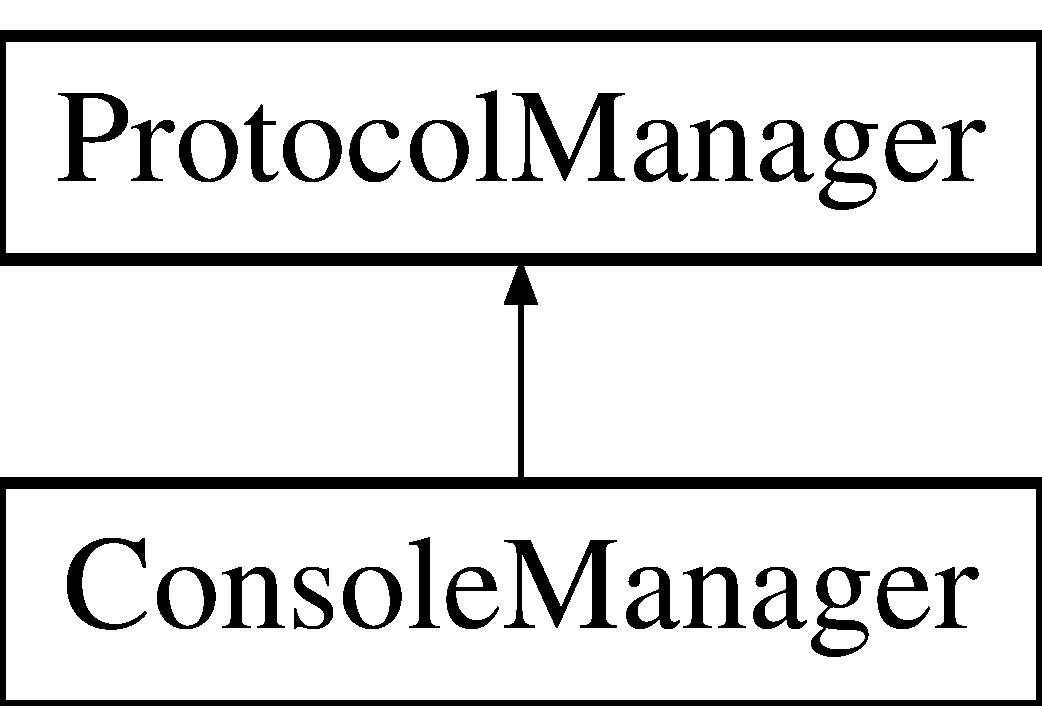
\includegraphics[height=2.000000cm]{classConsoleManager}
\end{center}
\end{figure}
\subsection*{Public Member Functions}
\begin{DoxyCompactItemize}
\item 
void \mbox{\hyperlink{classConsoleManager_a69261543a87cf7d3c7ec004c566145fd}{loop}} () override
\begin{DoxyCompactList}\small\item\em Starts the protocol loop. \end{DoxyCompactList}\item 
int32\+\_\+t \mbox{\hyperlink{classConsoleManager_a12c11521d46af302d6c7d79d3b8174b4}{get\+Protocol}} () override
\begin{DoxyCompactList}\small\item\em Returns the protocol identifier for the current protocol. \end{DoxyCompactList}\end{DoxyCompactItemize}
\subsection*{Additional Inherited Members}


\subsection{Detailed Description}
See \mbox{\hyperlink{classProtocolManager}{Protocol\+Manager}} documentation 

Definition at line 14 of file console.\+h.



\subsection{Member Function Documentation}
\mbox{\Hypertarget{classConsoleManager_a12c11521d46af302d6c7d79d3b8174b4}\label{classConsoleManager_a12c11521d46af302d6c7d79d3b8174b4}} 
\index{Console\+Manager@{Console\+Manager}!get\+Protocol@{get\+Protocol}}
\index{get\+Protocol@{get\+Protocol}!Console\+Manager@{Console\+Manager}}
\subsubsection{\texorpdfstring{get\+Protocol()}{getProtocol()}}
{\footnotesize\ttfamily int32\+\_\+t Console\+Manager\+::get\+Protocol (\begin{DoxyParamCaption}{ }\end{DoxyParamCaption})\hspace{0.3cm}{\ttfamily [override]}, {\ttfamily [virtual]}}



Returns the protocol identifier for the current protocol. 


\begin{DoxyParams}{Parameters}
{\em None} & \\
\hline
\end{DoxyParams}
\begin{DoxyReturn}{Returns}
The protocol identifier 
\end{DoxyReturn}


Implements \mbox{\hyperlink{classProtocolManager_a2ab274fd7510b28e7ac36405aebdbe82}{Protocol\+Manager}}.



Definition at line 191 of file console.\+cc.

\mbox{\Hypertarget{classConsoleManager_a69261543a87cf7d3c7ec004c566145fd}\label{classConsoleManager_a69261543a87cf7d3c7ec004c566145fd}} 
\index{Console\+Manager@{Console\+Manager}!loop@{loop}}
\index{loop@{loop}!Console\+Manager@{Console\+Manager}}
\subsubsection{\texorpdfstring{loop()}{loop()}}
{\footnotesize\ttfamily void Console\+Manager\+::loop (\begin{DoxyParamCaption}{ }\end{DoxyParamCaption})\hspace{0.3cm}{\ttfamily [override]}, {\ttfamily [virtual]}}



Starts the protocol loop. 


\begin{DoxyParams}{Parameters}
{\em None} & \\
\hline
\end{DoxyParams}
\begin{DoxyReturn}{Returns}
None 
\end{DoxyReturn}


Implements \mbox{\hyperlink{classProtocolManager_aa3ae25a03e2f070ea486fd9319715a6a}{Protocol\+Manager}}.



Definition at line 22 of file console.\+cc.



The documentation for this class was generated from the following files\+:\begin{DoxyCompactItemize}
\item 
include/\mbox{\hyperlink{console_8h}{console.\+h}}\item 
src/\mbox{\hyperlink{console_8cc}{console.\+cc}}\end{DoxyCompactItemize}

\hypertarget{classEngine}{}\section{Engine Class Reference}
\label{classEngine}\index{Engine@{Engine}}
\subsection*{Public Member Functions}
\begin{DoxyCompactItemize}
\item 
\mbox{\Hypertarget{classEngine_ab9ee0ddff1237cf61eb482bfce9ab480}\label{classEngine_ab9ee0ddff1237cf61eb482bfce9ab480}} 
{\bfseries Engine} (const \mbox{\hyperlink{classEngine}{Engine}} \&)=delete
\item 
\mbox{\Hypertarget{classEngine_a5d7e8ec8383567cfe24b2b94c5730729}\label{classEngine_a5d7e8ec8383567cfe24b2b94c5730729}} 
void {\bfseries operator=} (const \mbox{\hyperlink{classEngine}{Engine}} \&)=delete
\item 
\mbox{\Hypertarget{classEngine_aa78d58b978bb3c6bb147bc999e9523c1}\label{classEngine_aa78d58b978bb3c6bb147bc999e9523c1}} 
void {\bfseries start} () noexcept
\end{DoxyCompactItemize}
\subsection*{Static Public Member Functions}
\begin{DoxyCompactItemize}
\item 
\mbox{\Hypertarget{classEngine_ae174f8fa16fbab1633489283db2b0c9f}\label{classEngine_ae174f8fa16fbab1633489283db2b0c9f}} 
static \mbox{\hyperlink{classEngine}{Engine}} \& {\bfseries get\+Instance} ()
\item 
\mbox{\Hypertarget{classEngine_a0829ed04a1463100784500122bbe426f}\label{classEngine_a0829ed04a1463100784500122bbe426f}} 
static \mbox{\hyperlink{structEngineConfig}{Engine\+Config}} \& {\bfseries get\+Config} ()
\item 
\mbox{\Hypertarget{classEngine_a02d2a190f06bd06f23eb6ed02474f990}\label{classEngine_a02d2a190f06bd06f23eb6ed02474f990}} 
static \mbox{\hyperlink{classPolyBook}{Poly\+Book}} \& {\bfseries get\+Book} ()
\end{DoxyCompactItemize}
\subsection*{Private Member Functions}
\begin{DoxyCompactItemize}
\item 
\mbox{\Hypertarget{classEngine_a8402fb1995ca48ebb645b82bf943aac7}\label{classEngine_a8402fb1995ca48ebb645b82bf943aac7}} 
void {\bfseries print\+Greeting} () const noexcept
\end{DoxyCompactItemize}
\subsection*{Private Attributes}
\begin{DoxyCompactItemize}
\item 
\mbox{\Hypertarget{classEngine_a20ac20c3580244eced45e2f2f767a8da}\label{classEngine_a20ac20c3580244eced45e2f2f767a8da}} 
std\+::unique\+\_\+ptr$<$ \mbox{\hyperlink{classProtocolManager}{Protocol\+Manager}} $>$ {\bfseries protocol}
\item 
\mbox{\Hypertarget{classEngine_a63db1301ca47ea013b3fa83fd541a9aa}\label{classEngine_a63db1301ca47ea013b3fa83fd541a9aa}} 
\mbox{\hyperlink{structEngineConfig}{Engine\+Config}} {\bfseries config}
\item 
\mbox{\Hypertarget{classEngine_aa30f12ae58d51f051f22499f95c2602e}\label{classEngine_aa30f12ae58d51f051f22499f95c2602e}} 
\mbox{\hyperlink{classPolyBook}{Poly\+Book}} {\bfseries book}
\end{DoxyCompactItemize}


\subsection{Detailed Description}


Definition at line 19 of file engine.\+h.



The documentation for this class was generated from the following files\+:\begin{DoxyCompactItemize}
\item 
include/\mbox{\hyperlink{engine_8h}{engine.\+h}}\item 
src/\mbox{\hyperlink{engine_8cc}{engine.\+cc}}\end{DoxyCompactItemize}

\hypertarget{structEngineConfig}{}\section{Engine\+Config Struct Reference}
\label{structEngineConfig}\index{Engine\+Config@{Engine\+Config}}


Stores the flags for the engine.  




{\ttfamily \#include $<$engine.\+h$>$}

\subsection*{Data Fields}
\begin{DoxyCompactItemize}
\item 
\mbox{\Hypertarget{structEngineConfig_a6f6849a5e9919e75b34cd44b8a25a7bf}\label{structEngineConfig_a6f6849a5e9919e75b34cd44b8a25a7bf}} 
bool {\bfseries use\+Book}
\end{DoxyCompactItemize}


\subsection{Detailed Description}
Stores the flags for the engine. 

Definition at line 16 of file engine.\+h.



The documentation for this struct was generated from the following file\+:\begin{DoxyCompactItemize}
\item 
/home/michael/\+Documents/\+Projects/\+C++/\+Chess-\/\+Engine/include/\mbox{\hyperlink{engine_8h}{engine.\+h}}\end{DoxyCompactItemize}

\hypertarget{classEvaluator}{}\section{Evaluator Class Reference}
\label{classEvaluator}\index{Evaluator@{Evaluator}}
\subsection*{Public Member Functions}
\begin{DoxyCompactItemize}
\item 
int32\+\_\+t \mbox{\hyperlink{classEvaluator_a82ac01bb85da704f7a9f1a059c0e91fb}{evaluate\+Position}} (const \mbox{\hyperlink{classBoard}{Board}} \&pos) noexcept
\begin{DoxyCompactList}\small\item\em Evaluates the score for the current board position for the side to move. \end{DoxyCompactList}\end{DoxyCompactItemize}
\subsection*{Private Member Functions}
\begin{DoxyCompactItemize}
\item 
int32\+\_\+t \mbox{\hyperlink{classEvaluator_a76e81d148449a9bb6c1616895223ad77}{eval\+Pawns}} (const \mbox{\hyperlink{classBoard}{Board}} \&pos) noexcept
\begin{DoxyCompactList}\small\item\em Evaluates the strength of the Pawns. \end{DoxyCompactList}\item 
int32\+\_\+t \mbox{\hyperlink{classEvaluator_ab8235a37e631665e0dbdbffdddf015f7}{eval\+Bishops}} (const \mbox{\hyperlink{classBoard}{Board}} \&pos) noexcept
\begin{DoxyCompactList}\small\item\em Evaluates the strength of the Bishop. \end{DoxyCompactList}\item 
int32\+\_\+t \mbox{\hyperlink{classEvaluator_ac1cfc6e10fcd71fc4148415d889a4085}{eval\+Rooks}} (const \mbox{\hyperlink{classBoard}{Board}} \&pos) noexcept
\begin{DoxyCompactList}\small\item\em Evaluates the strength of the Rook. \end{DoxyCompactList}\item 
int32\+\_\+t \mbox{\hyperlink{classEvaluator_aaf81df6872cb3c5acabc05b4865c4bcd}{eval\+Knights}} (const \mbox{\hyperlink{classBoard}{Board}} \&pos) noexcept
\begin{DoxyCompactList}\small\item\em Evaluates the strength of the Knights. \end{DoxyCompactList}\item 
int32\+\_\+t \mbox{\hyperlink{classEvaluator_a322d577548dd00c32e949cad62a17393}{eval\+Queens}} (const \mbox{\hyperlink{classBoard}{Board}} \&pos) noexcept
\begin{DoxyCompactList}\small\item\em Evaluates the strength of the Queens. \end{DoxyCompactList}\item 
int32\+\_\+t \mbox{\hyperlink{classEvaluator_af8971fc82010e0a08a1e510847bf304c}{eval\+Kings}} (const \mbox{\hyperlink{classBoard}{Board}} \&pos) noexcept
\begin{DoxyCompactList}\small\item\em Evaluates the strength of the Kings. \end{DoxyCompactList}\item 
bool \mbox{\hyperlink{classEvaluator_aec21b1e28f162b7f1e4edc9e8f725a8b}{drawn\+Material}} (const \mbox{\hyperlink{classBoard}{Board}} \&pos) noexcept
\begin{DoxyCompactList}\small\item\em Determines if there is enough material to end in checkmate. \end{DoxyCompactList}\end{DoxyCompactItemize}


\subsection{Detailed Description}


Definition at line 159 of file eval.\+h.



\subsection{Member Function Documentation}
\mbox{\Hypertarget{classEvaluator_aec21b1e28f162b7f1e4edc9e8f725a8b}\label{classEvaluator_aec21b1e28f162b7f1e4edc9e8f725a8b}} 
\index{Evaluator@{Evaluator}!drawn\+Material@{drawn\+Material}}
\index{drawn\+Material@{drawn\+Material}!Evaluator@{Evaluator}}
\subsubsection{\texorpdfstring{drawn\+Material()}{drawnMaterial()}}
{\footnotesize\ttfamily bool Evaluator\+::drawn\+Material (\begin{DoxyParamCaption}\item[{const \mbox{\hyperlink{classBoard}{Board}} \&}]{pos }\end{DoxyParamCaption})\hspace{0.3cm}{\ttfamily [private]}, {\ttfamily [noexcept]}}



Determines if there is enough material to end in checkmate. 


\begin{DoxyParams}{Parameters}
{\em pos} & The current board state. \\
\hline
\end{DoxyParams}
\begin{DoxyReturn}{Returns}
true if there is enough material on either side to lead to checkmate, false otherwise. 
\end{DoxyReturn}


Definition at line 188 of file eval.\+cc.

\mbox{\Hypertarget{classEvaluator_ab8235a37e631665e0dbdbffdddf015f7}\label{classEvaluator_ab8235a37e631665e0dbdbffdddf015f7}} 
\index{Evaluator@{Evaluator}!eval\+Bishops@{eval\+Bishops}}
\index{eval\+Bishops@{eval\+Bishops}!Evaluator@{Evaluator}}
\subsubsection{\texorpdfstring{eval\+Bishops()}{evalBishops()}}
{\footnotesize\ttfamily int32\+\_\+t Evaluator\+::eval\+Bishops (\begin{DoxyParamCaption}\item[{const \mbox{\hyperlink{classBoard}{Board}} \&}]{pos }\end{DoxyParamCaption})\hspace{0.3cm}{\ttfamily [private]}, {\ttfamily [noexcept]}}



Evaluates the strength of the Bishop. 


\begin{DoxyParams}{Parameters}
{\em pos} & The current board state. \\
\hline
\end{DoxyParams}
\begin{DoxyReturn}{Returns}
The score attributed to the Bishop. 
\end{DoxyReturn}


Definition at line 52 of file eval.\+cc.

\mbox{\Hypertarget{classEvaluator_af8971fc82010e0a08a1e510847bf304c}\label{classEvaluator_af8971fc82010e0a08a1e510847bf304c}} 
\index{Evaluator@{Evaluator}!eval\+Kings@{eval\+Kings}}
\index{eval\+Kings@{eval\+Kings}!Evaluator@{Evaluator}}
\subsubsection{\texorpdfstring{eval\+Kings()}{evalKings()}}
{\footnotesize\ttfamily int32\+\_\+t Evaluator\+::eval\+Kings (\begin{DoxyParamCaption}\item[{const \mbox{\hyperlink{classBoard}{Board}} \&}]{pos }\end{DoxyParamCaption})\hspace{0.3cm}{\ttfamily [private]}, {\ttfamily [noexcept]}}



Evaluates the strength of the Kings. 


\begin{DoxyParams}{Parameters}
{\em pos} & The current board state. \\
\hline
\end{DoxyParams}
\begin{DoxyReturn}{Returns}
The score attributed to the Kings. 
\end{DoxyReturn}


Definition at line 142 of file eval.\+cc.

\mbox{\Hypertarget{classEvaluator_aaf81df6872cb3c5acabc05b4865c4bcd}\label{classEvaluator_aaf81df6872cb3c5acabc05b4865c4bcd}} 
\index{Evaluator@{Evaluator}!eval\+Knights@{eval\+Knights}}
\index{eval\+Knights@{eval\+Knights}!Evaluator@{Evaluator}}
\subsubsection{\texorpdfstring{eval\+Knights()}{evalKnights()}}
{\footnotesize\ttfamily int32\+\_\+t Evaluator\+::eval\+Knights (\begin{DoxyParamCaption}\item[{const \mbox{\hyperlink{classBoard}{Board}} \&}]{pos }\end{DoxyParamCaption})\hspace{0.3cm}{\ttfamily [private]}, {\ttfamily [noexcept]}}



Evaluates the strength of the Knights. 


\begin{DoxyParams}{Parameters}
{\em pos} & The current board state. \\
\hline
\end{DoxyParams}
\begin{DoxyReturn}{Returns}
The score attributed to the Knights. 
\end{DoxyReturn}


Definition at line 171 of file eval.\+cc.

\mbox{\Hypertarget{classEvaluator_a76e81d148449a9bb6c1616895223ad77}\label{classEvaluator_a76e81d148449a9bb6c1616895223ad77}} 
\index{Evaluator@{Evaluator}!eval\+Pawns@{eval\+Pawns}}
\index{eval\+Pawns@{eval\+Pawns}!Evaluator@{Evaluator}}
\subsubsection{\texorpdfstring{eval\+Pawns()}{evalPawns()}}
{\footnotesize\ttfamily int32\+\_\+t Evaluator\+::eval\+Pawns (\begin{DoxyParamCaption}\item[{const \mbox{\hyperlink{classBoard}{Board}} \&}]{pos }\end{DoxyParamCaption})\hspace{0.3cm}{\ttfamily [private]}, {\ttfamily [noexcept]}}



Evaluates the strength of the Pawns. 


\begin{DoxyParams}{Parameters}
{\em pos} & The current board state. \\
\hline
\end{DoxyParams}
\begin{DoxyReturn}{Returns}
The score attributed to the Pawns. 
\end{DoxyReturn}


Definition at line 14 of file eval.\+cc.

\mbox{\Hypertarget{classEvaluator_a322d577548dd00c32e949cad62a17393}\label{classEvaluator_a322d577548dd00c32e949cad62a17393}} 
\index{Evaluator@{Evaluator}!eval\+Queens@{eval\+Queens}}
\index{eval\+Queens@{eval\+Queens}!Evaluator@{Evaluator}}
\subsubsection{\texorpdfstring{eval\+Queens()}{evalQueens()}}
{\footnotesize\ttfamily int32\+\_\+t Evaluator\+::eval\+Queens (\begin{DoxyParamCaption}\item[{const \mbox{\hyperlink{classBoard}{Board}} \&}]{pos }\end{DoxyParamCaption})\hspace{0.3cm}{\ttfamily [private]}, {\ttfamily [noexcept]}}



Evaluates the strength of the Queens. 


\begin{DoxyParams}{Parameters}
{\em pos} & The current board state. \\
\hline
\end{DoxyParams}
\begin{DoxyReturn}{Returns}
The score attributed to the Queens. 
\end{DoxyReturn}


Definition at line 108 of file eval.\+cc.

\mbox{\Hypertarget{classEvaluator_ac1cfc6e10fcd71fc4148415d889a4085}\label{classEvaluator_ac1cfc6e10fcd71fc4148415d889a4085}} 
\index{Evaluator@{Evaluator}!eval\+Rooks@{eval\+Rooks}}
\index{eval\+Rooks@{eval\+Rooks}!Evaluator@{Evaluator}}
\subsubsection{\texorpdfstring{eval\+Rooks()}{evalRooks()}}
{\footnotesize\ttfamily int32\+\_\+t Evaluator\+::eval\+Rooks (\begin{DoxyParamCaption}\item[{const \mbox{\hyperlink{classBoard}{Board}} \&}]{pos }\end{DoxyParamCaption})\hspace{0.3cm}{\ttfamily [private]}, {\ttfamily [noexcept]}}



Evaluates the strength of the Rook. 


\begin{DoxyParams}{Parameters}
{\em pos} & The current board state. \\
\hline
\end{DoxyParams}
\begin{DoxyReturn}{Returns}
The score attributed to the Rook. 
\end{DoxyReturn}


Definition at line 72 of file eval.\+cc.

\mbox{\Hypertarget{classEvaluator_a82ac01bb85da704f7a9f1a059c0e91fb}\label{classEvaluator_a82ac01bb85da704f7a9f1a059c0e91fb}} 
\index{Evaluator@{Evaluator}!evaluate\+Position@{evaluate\+Position}}
\index{evaluate\+Position@{evaluate\+Position}!Evaluator@{Evaluator}}
\subsubsection{\texorpdfstring{evaluate\+Position()}{evaluatePosition()}}
{\footnotesize\ttfamily int32\+\_\+t Evaluator\+::evaluate\+Position (\begin{DoxyParamCaption}\item[{const \mbox{\hyperlink{classBoard}{Board}} \&}]{pos }\end{DoxyParamCaption})\hspace{0.3cm}{\ttfamily [noexcept]}}



Evaluates the score for the current board position for the side to move. 


\begin{DoxyParams}{Parameters}
{\em pos} & The current board state. \\
\hline
\end{DoxyParams}
\begin{DoxyReturn}{Returns}
The overall score of the position 
\end{DoxyReturn}


Definition at line 243 of file eval.\+cc.



The documentation for this class was generated from the following files\+:\begin{DoxyCompactItemize}
\item 
/home/michael/\+Documents/\+Projects/\+C++/\+Chess-\/\+Engine/include/\mbox{\hyperlink{eval_8h}{eval.\+h}}\item 
/home/michael/\+Documents/\+Projects/\+C++/\+Chess-\/\+Engine/src/\mbox{\hyperlink{eval_8cc}{eval.\+cc}}\end{DoxyCompactItemize}

\hypertarget{classMM}{}\section{MM Class Reference}
\label{classMM}\index{MM@{MM}}
\subsection*{Static Public Member Functions}
\begin{DoxyCompactItemize}
\item 
static bool \mbox{\hyperlink{classMM_ad56f88355a078f3b14b290fe153966b4}{make\+Move}} (\mbox{\hyperlink{classBoard}{Board}} \&pos, const \mbox{\hyperlink{classMove}{Move}} \&move\+Info) noexcept
\begin{DoxyCompactList}\small\item\em Makes the provided move (move piece/capture/update board) \end{DoxyCompactList}\item 
static void \mbox{\hyperlink{classMM_aaf252571e1f48cae22b2093bf55058b5}{take\+Move}} (\mbox{\hyperlink{classBoard}{Board}} \&pos) noexcept
\begin{DoxyCompactList}\small\item\em Undos the last move that was made which is stored in Board\+::history. \end{DoxyCompactList}\item 
static void \mbox{\hyperlink{classMM_a363e843e6bebaf747bf9482c963ed6b9}{make\+Null\+Move}} (\mbox{\hyperlink{classBoard}{Board}} \&pos) noexcept
\begin{DoxyCompactList}\small\item\em Similar in concept to Make move, but gives the opposing side a free move. \end{DoxyCompactList}\item 
static void \mbox{\hyperlink{classMM_aabe809e8405f8ea0666a7d6e25aedac5}{take\+Null\+Move}} (\mbox{\hyperlink{classBoard}{Board}} \&pos) noexcept
\begin{DoxyCompactList}\small\item\em Undos the last null move. \end{DoxyCompactList}\end{DoxyCompactItemize}
\subsection*{Static Private Member Functions}
\begin{DoxyCompactItemize}
\item 
static void \mbox{\hyperlink{classMM_a590ca1cb1afc08df645f947e48c13e0c}{clear\+Piece}} (const uint32\+\_\+t sq, \mbox{\hyperlink{classBoard}{Board}} \&pos) noexcept
\begin{DoxyCompactList}\small\item\em Removes the piece on the given square from the internal board representation. \end{DoxyCompactList}\item 
static void \mbox{\hyperlink{classMM_a2f50160abe49fcba984c0db8cca3a2e4}{add\+Piece}} (const uint32\+\_\+t sq, \mbox{\hyperlink{classBoard}{Board}} \&pos, const uint32\+\_\+t pce) noexcept
\begin{DoxyCompactList}\small\item\em Adds the piece on the given square to the internal board representation. \end{DoxyCompactList}\item 
static void \mbox{\hyperlink{classMM_a0a47ca15cd28a2b8136e7be86aff84e7}{move\+Piece}} (const uint32\+\_\+t src, const uint32\+\_\+t dest, \mbox{\hyperlink{classBoard}{Board}} \&pos) noexcept
\begin{DoxyCompactList}\small\item\em Moves the piece from the source square to the dest square and performs capture if applicable. \end{DoxyCompactList}\end{DoxyCompactItemize}


\subsection{Detailed Description}


Definition at line 34 of file movemaker.\+h.



\subsection{Member Function Documentation}
\mbox{\Hypertarget{classMM_a2f50160abe49fcba984c0db8cca3a2e4}\label{classMM_a2f50160abe49fcba984c0db8cca3a2e4}} 
\index{MM@{MM}!add\+Piece@{add\+Piece}}
\index{add\+Piece@{add\+Piece}!MM@{MM}}
\subsubsection{\texorpdfstring{add\+Piece()}{addPiece()}}
{\footnotesize\ttfamily void M\+M\+::add\+Piece (\begin{DoxyParamCaption}\item[{const uint32\+\_\+t}]{sq,  }\item[{\mbox{\hyperlink{classBoard}{Board}} \&}]{pos,  }\item[{const uint32\+\_\+t}]{pce }\end{DoxyParamCaption})\hspace{0.3cm}{\ttfamily [static]}, {\ttfamily [private]}, {\ttfamily [noexcept]}}



Adds the piece on the given square to the internal board representation. 


\begin{DoxyParams}{Parameters}
{\em sq} & The square to add the piece to. \\
\hline
{\em pos} & The current board state. \\
\hline
{\em pce} & The piece to add to the target square \\
\hline
\end{DoxyParams}
\begin{DoxyReturn}{Returns}
None 
\end{DoxyReturn}


Definition at line 47 of file movemaker.\+cc.

\mbox{\Hypertarget{classMM_a590ca1cb1afc08df645f947e48c13e0c}\label{classMM_a590ca1cb1afc08df645f947e48c13e0c}} 
\index{MM@{MM}!clear\+Piece@{clear\+Piece}}
\index{clear\+Piece@{clear\+Piece}!MM@{MM}}
\subsubsection{\texorpdfstring{clear\+Piece()}{clearPiece()}}
{\footnotesize\ttfamily void M\+M\+::clear\+Piece (\begin{DoxyParamCaption}\item[{const uint32\+\_\+t}]{sq,  }\item[{\mbox{\hyperlink{classBoard}{Board}} \&}]{pos }\end{DoxyParamCaption})\hspace{0.3cm}{\ttfamily [static]}, {\ttfamily [private]}, {\ttfamily [noexcept]}}



Removes the piece on the given square from the internal board representation. 


\begin{DoxyParams}{Parameters}
{\em sq} & The square to clear. \\
\hline
{\em pos} & The current board state. \\
\hline
\end{DoxyParams}
\begin{DoxyReturn}{Returns}
None 
\end{DoxyReturn}


Definition at line 20 of file movemaker.\+cc.

\mbox{\Hypertarget{classMM_ad56f88355a078f3b14b290fe153966b4}\label{classMM_ad56f88355a078f3b14b290fe153966b4}} 
\index{MM@{MM}!make\+Move@{make\+Move}}
\index{make\+Move@{make\+Move}!MM@{MM}}
\subsubsection{\texorpdfstring{make\+Move()}{makeMove()}}
{\footnotesize\ttfamily bool M\+M\+::make\+Move (\begin{DoxyParamCaption}\item[{\mbox{\hyperlink{classBoard}{Board}} \&}]{pos,  }\item[{const \mbox{\hyperlink{classMove}{Move}} \&}]{move\+Info }\end{DoxyParamCaption})\hspace{0.3cm}{\ttfamily [static]}, {\ttfamily [noexcept]}}



Makes the provided move (move piece/capture/update board) 


\begin{DoxyParams}{Parameters}
{\em pos} & The current board state. \\
\hline
\end{DoxyParams}
\begin{DoxyReturn}{Returns}
true if move was successfully made (legal), false otherwise 
\end{DoxyReturn}


Definition at line 92 of file movemaker.\+cc.

\mbox{\Hypertarget{classMM_a363e843e6bebaf747bf9482c963ed6b9}\label{classMM_a363e843e6bebaf747bf9482c963ed6b9}} 
\index{MM@{MM}!make\+Null\+Move@{make\+Null\+Move}}
\index{make\+Null\+Move@{make\+Null\+Move}!MM@{MM}}
\subsubsection{\texorpdfstring{make\+Null\+Move()}{makeNullMove()}}
{\footnotesize\ttfamily void M\+M\+::make\+Null\+Move (\begin{DoxyParamCaption}\item[{\mbox{\hyperlink{classBoard}{Board}} \&}]{pos }\end{DoxyParamCaption})\hspace{0.3cm}{\ttfamily [static]}, {\ttfamily [noexcept]}}



Similar in concept to Make move, but gives the opposing side a free move. 


\begin{DoxyParams}{Parameters}
{\em pos} & The current board state. \\
\hline
\end{DoxyParams}
\begin{DoxyReturn}{Returns}
None 
\end{DoxyReturn}


Definition at line 251 of file movemaker.\+cc.

\mbox{\Hypertarget{classMM_a0a47ca15cd28a2b8136e7be86aff84e7}\label{classMM_a0a47ca15cd28a2b8136e7be86aff84e7}} 
\index{MM@{MM}!move\+Piece@{move\+Piece}}
\index{move\+Piece@{move\+Piece}!MM@{MM}}
\subsubsection{\texorpdfstring{move\+Piece()}{movePiece()}}
{\footnotesize\ttfamily void M\+M\+::move\+Piece (\begin{DoxyParamCaption}\item[{const uint32\+\_\+t}]{src,  }\item[{const uint32\+\_\+t}]{dest,  }\item[{\mbox{\hyperlink{classBoard}{Board}} \&}]{pos }\end{DoxyParamCaption})\hspace{0.3cm}{\ttfamily [static]}, {\ttfamily [private]}, {\ttfamily [noexcept]}}



Moves the piece from the source square to the dest square and performs capture if applicable. 


\begin{DoxyParams}{Parameters}
{\em src} & The square the piece starts on. \\
\hline
{\em dest} & The square the piece is moving to. \\
\hline
{\em pos} & The current board state. \\
\hline
\end{DoxyParams}
\begin{DoxyReturn}{Returns}
None 
\end{DoxyReturn}


Definition at line 73 of file movemaker.\+cc.

\mbox{\Hypertarget{classMM_aaf252571e1f48cae22b2093bf55058b5}\label{classMM_aaf252571e1f48cae22b2093bf55058b5}} 
\index{MM@{MM}!take\+Move@{take\+Move}}
\index{take\+Move@{take\+Move}!MM@{MM}}
\subsubsection{\texorpdfstring{take\+Move()}{takeMove()}}
{\footnotesize\ttfamily void M\+M\+::take\+Move (\begin{DoxyParamCaption}\item[{\mbox{\hyperlink{classBoard}{Board}} \&}]{pos }\end{DoxyParamCaption})\hspace{0.3cm}{\ttfamily [static]}, {\ttfamily [noexcept]}}



Undos the last move that was made which is stored in Board\+::history. 


\begin{DoxyParams}{Parameters}
{\em pos} & The current board state. \\
\hline
\end{DoxyParams}
\begin{DoxyReturn}{Returns}
None 
\end{DoxyReturn}


Definition at line 181 of file movemaker.\+cc.

\mbox{\Hypertarget{classMM_aabe809e8405f8ea0666a7d6e25aedac5}\label{classMM_aabe809e8405f8ea0666a7d6e25aedac5}} 
\index{MM@{MM}!take\+Null\+Move@{take\+Null\+Move}}
\index{take\+Null\+Move@{take\+Null\+Move}!MM@{MM}}
\subsubsection{\texorpdfstring{take\+Null\+Move()}{takeNullMove()}}
{\footnotesize\ttfamily void M\+M\+::take\+Null\+Move (\begin{DoxyParamCaption}\item[{\mbox{\hyperlink{classBoard}{Board}} \&}]{pos }\end{DoxyParamCaption})\hspace{0.3cm}{\ttfamily [static]}, {\ttfamily [noexcept]}}



Undos the last null move. 


\begin{DoxyParams}{Parameters}
{\em pos} & The current board state. \\
\hline
\end{DoxyParams}
\begin{DoxyReturn}{Returns}
None 
\end{DoxyReturn}


Definition at line 274 of file movemaker.\+cc.



The documentation for this class was generated from the following files\+:\begin{DoxyCompactItemize}
\item 
/home/michael/\+Documents/\+Projects/\+C++/\+Chess-\/\+Engine/include/\mbox{\hyperlink{movemaker_8h}{movemaker.\+h}}\item 
/home/michael/\+Documents/\+Projects/\+C++/\+Chess-\/\+Engine/src/\mbox{\hyperlink{movemaker_8cc}{movemaker.\+cc}}\end{DoxyCompactItemize}

\hypertarget{classMove}{}\section{Move Class Reference}
\label{classMove}\index{Move@{Move}}
\subsection*{Public Member Functions}
\begin{DoxyCompactItemize}
\item 
\mbox{\Hypertarget{classMove_ac63ab436cc90ca3b83f6bf9328745410}\label{classMove_ac63ab436cc90ca3b83f6bf9328745410}} 
{\bfseries Move} (uint32\+\_\+t \mbox{\hyperlink{classMove_a5a16b2160e1cb66cde53dd6251616243}{from}}, uint32\+\_\+t \mbox{\hyperlink{classMove_a14f68402d1ad19b441730a7f7d703362}{to}}, uint32\+\_\+t \mbox{\hyperlink{classMove_a5a8811a7e6ee7fe36675d49038f2ea2b}{captured}}, uint32\+\_\+t prom, uint32\+\_\+t flag) noexcept
\item 
\mbox{\Hypertarget{classMove_a880d0197342959b353fd6de7d0cae16f}\label{classMove_a880d0197342959b353fd6de7d0cae16f}} 
{\bfseries Move} (uint32\+\_\+t \+\_\+move, int32\+\_\+t \+\_\+score) noexcept
\item 
\mbox{\Hypertarget{classMove_a023d4469f67a68d9d39ce24b95031ab8}\label{classMove_a023d4469f67a68d9d39ce24b95031ab8}} 
{\bfseries Move} (uint32\+\_\+t \+\_\+move) noexcept
\item 
\mbox{\Hypertarget{classMove_a29a98334b21446eba8df130c2521b13f}\label{classMove_a29a98334b21446eba8df130c2521b13f}} 
{\bfseries Move} (const \mbox{\hyperlink{classMove}{Move}} \&o) noexcept
\item 
\mbox{\Hypertarget{classMove_a84c4266bc47d32d7c07a72f76c2d2e46}\label{classMove_a84c4266bc47d32d7c07a72f76c2d2e46}} 
{\bfseries Move} (\mbox{\hyperlink{classMove}{Move}} \&\&o) noexcept
\item 
constexpr uint32\+\_\+t \mbox{\hyperlink{classMove_a5a16b2160e1cb66cde53dd6251616243}{from}} () const
\begin{DoxyCompactList}\small\item\em Gets the square that the move is starting from. \end{DoxyCompactList}\item 
constexpr uint32\+\_\+t \mbox{\hyperlink{classMove_a14f68402d1ad19b441730a7f7d703362}{to}} () const
\begin{DoxyCompactList}\small\item\em Gets the square that the move is ending on. \end{DoxyCompactList}\item 
constexpr uint32\+\_\+t \mbox{\hyperlink{classMove_a5a8811a7e6ee7fe36675d49038f2ea2b}{captured}} () const
\begin{DoxyCompactList}\small\item\em Gets the piece That was captured. \end{DoxyCompactList}\item 
constexpr uint32\+\_\+t \mbox{\hyperlink{classMove_a69a64f5ba158cf0f48765ea40de0daf0}{en\+Passant}} () const
\begin{DoxyCompactList}\small\item\em Checks if the move was an En\+Passant move. \end{DoxyCompactList}\item 
constexpr uint32\+\_\+t \mbox{\hyperlink{classMove_ae9eaee49438859900541d7a308161a8b}{pawn\+Start}} () const
\begin{DoxyCompactList}\small\item\em Checks if the move was a pawn start (pawn double move). \end{DoxyCompactList}\item 
constexpr uint32\+\_\+t \mbox{\hyperlink{classMove_a68741632b4a38ae64152541ed3c641ae}{promoted}} () const
\begin{DoxyCompactList}\small\item\em Gets the piece that was promoted to if any. \end{DoxyCompactList}\item 
constexpr uint32\+\_\+t \mbox{\hyperlink{classMove_a35d7341c2a9074102451bf4df0d8b4c2}{castle}} () const
\begin{DoxyCompactList}\small\item\em Checks if the move was a castle move. \end{DoxyCompactList}\item 
constexpr bool \mbox{\hyperlink{classMove_ac986baf2580e64f47828c8adf23a25f0}{is\+Null}} () const
\begin{DoxyCompactList}\small\item\em Checks if the move was N\+U\+L\+L\+M\+O\+VE. \end{DoxyCompactList}\item 
constexpr bool \mbox{\hyperlink{classMove_aa270da1cc5c6f10882cd14e9a61d2ebe}{was\+Capture}} () const
\begin{DoxyCompactList}\small\item\em Checks if the move was a capture. \end{DoxyCompactList}\item 
constexpr bool \mbox{\hyperlink{classMove_a06483745a13016873fc99db2ea74e042}{was\+Promotion}} () const
\begin{DoxyCompactList}\small\item\em Checks if the move was a promotion. \end{DoxyCompactList}\item 
const std\+::string \mbox{\hyperlink{classMove_a521cf6fe1679a7354ee007037df2da34}{to\+String}} () const noexcept
\begin{DoxyCompactList}\small\item\em Gets the string representation of a move (e.\+g \char`\"{}e2e4\char`\"{}). \end{DoxyCompactList}\item 
\mbox{\Hypertarget{classMove_a9474c9aae57d49cc2e74dfcd3466a62f}\label{classMove_a9474c9aae57d49cc2e74dfcd3466a62f}} 
\mbox{\hyperlink{classMove}{Move}} \& {\bfseries operator=} (const \mbox{\hyperlink{classMove}{Move}} \&o) noexcept
\item 
\mbox{\Hypertarget{classMove_a14f146246c87d23b4b6f8d4853868436}\label{classMove_a14f146246c87d23b4b6f8d4853868436}} 
\mbox{\hyperlink{classMove}{Move}} \& {\bfseries operator=} (\mbox{\hyperlink{classMove}{Move}} \&\&o) noexcept
\item 
\mbox{\Hypertarget{classMove_abe04723add8693b51f92d5f11e5a350a}\label{classMove_abe04723add8693b51f92d5f11e5a350a}} 
bool {\bfseries operator==} (const \mbox{\hyperlink{classMove}{Move}} \&rhs) const noexcept
\item 
\mbox{\Hypertarget{classMove_a1d317f2b6d8bf51a825319f8ceacdd27}\label{classMove_a1d317f2b6d8bf51a825319f8ceacdd27}} 
bool {\bfseries operator!=} (const \mbox{\hyperlink{classMove}{Move}} \&rhs) const noexcept
\end{DoxyCompactItemize}
\subsection*{Data Fields}
\begin{DoxyCompactItemize}
\item 
\mbox{\Hypertarget{classMove_a05c0d1c118aaccb4928569c740ecdb5f}\label{classMove_a05c0d1c118aaccb4928569c740ecdb5f}} 
uint32\+\_\+t {\bfseries move}
\item 
\mbox{\Hypertarget{classMove_a910be8d231eabe9a9cd98988f1274538}\label{classMove_a910be8d231eabe9a9cd98988f1274538}} 
int32\+\_\+t {\bfseries score}
\end{DoxyCompactItemize}


\subsection{Detailed Description}


Definition at line 40 of file move.\+h.



\subsection{Member Function Documentation}
\mbox{\Hypertarget{classMove_a5a8811a7e6ee7fe36675d49038f2ea2b}\label{classMove_a5a8811a7e6ee7fe36675d49038f2ea2b}} 
\index{Move@{Move}!captured@{captured}}
\index{captured@{captured}!Move@{Move}}
\subsubsection{\texorpdfstring{captured()}{captured()}}
{\footnotesize\ttfamily constexpr uint32\+\_\+t Move\+::captured (\begin{DoxyParamCaption}{ }\end{DoxyParamCaption}) const\hspace{0.3cm}{\ttfamily [inline]}}



Gets the piece That was captured. 


\begin{DoxyParams}{Parameters}
{\em None} & \\
\hline
\end{DoxyParams}
\begin{DoxyReturn}{Returns}
The piece that was captured. 
\end{DoxyReturn}


Definition at line 69 of file move.\+h.

\mbox{\Hypertarget{classMove_a35d7341c2a9074102451bf4df0d8b4c2}\label{classMove_a35d7341c2a9074102451bf4df0d8b4c2}} 
\index{Move@{Move}!castle@{castle}}
\index{castle@{castle}!Move@{Move}}
\subsubsection{\texorpdfstring{castle()}{castle()}}
{\footnotesize\ttfamily constexpr uint32\+\_\+t Move\+::castle (\begin{DoxyParamCaption}{ }\end{DoxyParamCaption}) const\hspace{0.3cm}{\ttfamily [inline]}}



Checks if the move was a castle move. 


\begin{DoxyParams}{Parameters}
{\em None} & \\
\hline
\end{DoxyParams}
\begin{DoxyReturn}{Returns}
true if there was a castle move, false otherwise. 
\end{DoxyReturn}


Definition at line 93 of file move.\+h.

\mbox{\Hypertarget{classMove_a69a64f5ba158cf0f48765ea40de0daf0}\label{classMove_a69a64f5ba158cf0f48765ea40de0daf0}} 
\index{Move@{Move}!en\+Passant@{en\+Passant}}
\index{en\+Passant@{en\+Passant}!Move@{Move}}
\subsubsection{\texorpdfstring{en\+Passant()}{enPassant()}}
{\footnotesize\ttfamily constexpr uint32\+\_\+t Move\+::en\+Passant (\begin{DoxyParamCaption}{ }\end{DoxyParamCaption}) const\hspace{0.3cm}{\ttfamily [inline]}}



Checks if the move was an En\+Passant move. 


\begin{DoxyParams}{Parameters}
{\em None} & \\
\hline
\end{DoxyParams}
\begin{DoxyReturn}{Returns}
true if there was En\+Passant, false otherwise. 
\end{DoxyReturn}


Definition at line 75 of file move.\+h.

\mbox{\Hypertarget{classMove_a5a16b2160e1cb66cde53dd6251616243}\label{classMove_a5a16b2160e1cb66cde53dd6251616243}} 
\index{Move@{Move}!from@{from}}
\index{from@{from}!Move@{Move}}
\subsubsection{\texorpdfstring{from()}{from()}}
{\footnotesize\ttfamily constexpr uint32\+\_\+t Move\+::from (\begin{DoxyParamCaption}{ }\end{DoxyParamCaption}) const\hspace{0.3cm}{\ttfamily [inline]}}



Gets the square that the move is starting from. 


\begin{DoxyParams}{Parameters}
{\em None} & \\
\hline
\end{DoxyParams}
\begin{DoxyReturn}{Returns}
The source square 
\end{DoxyReturn}


Definition at line 57 of file move.\+h.

\mbox{\Hypertarget{classMove_ac986baf2580e64f47828c8adf23a25f0}\label{classMove_ac986baf2580e64f47828c8adf23a25f0}} 
\index{Move@{Move}!is\+Null@{is\+Null}}
\index{is\+Null@{is\+Null}!Move@{Move}}
\subsubsection{\texorpdfstring{is\+Null()}{isNull()}}
{\footnotesize\ttfamily constexpr bool Move\+::is\+Null (\begin{DoxyParamCaption}{ }\end{DoxyParamCaption}) const\hspace{0.3cm}{\ttfamily [inline]}}



Checks if the move was N\+U\+L\+L\+M\+O\+VE. 


\begin{DoxyParams}{Parameters}
{\em None} & \\
\hline
\end{DoxyParams}
\begin{DoxyReturn}{Returns}
true if ($\ast$this) == N\+U\+L\+L\+M\+O\+VE, false otherwise. 
\end{DoxyReturn}


Definition at line 100 of file move.\+h.

\mbox{\Hypertarget{classMove_ae9eaee49438859900541d7a308161a8b}\label{classMove_ae9eaee49438859900541d7a308161a8b}} 
\index{Move@{Move}!pawn\+Start@{pawn\+Start}}
\index{pawn\+Start@{pawn\+Start}!Move@{Move}}
\subsubsection{\texorpdfstring{pawn\+Start()}{pawnStart()}}
{\footnotesize\ttfamily constexpr uint32\+\_\+t Move\+::pawn\+Start (\begin{DoxyParamCaption}{ }\end{DoxyParamCaption}) const\hspace{0.3cm}{\ttfamily [inline]}}



Checks if the move was a pawn start (pawn double move). 


\begin{DoxyParams}{Parameters}
{\em None} & \\
\hline
\end{DoxyParams}
\begin{DoxyReturn}{Returns}
true if there was a pawn start, false otherwise. 
\end{DoxyReturn}


Definition at line 81 of file move.\+h.

\mbox{\Hypertarget{classMove_a68741632b4a38ae64152541ed3c641ae}\label{classMove_a68741632b4a38ae64152541ed3c641ae}} 
\index{Move@{Move}!promoted@{promoted}}
\index{promoted@{promoted}!Move@{Move}}
\subsubsection{\texorpdfstring{promoted()}{promoted()}}
{\footnotesize\ttfamily constexpr uint32\+\_\+t Move\+::promoted (\begin{DoxyParamCaption}{ }\end{DoxyParamCaption}) const\hspace{0.3cm}{\ttfamily [inline]}}



Gets the piece that was promoted to if any. 


\begin{DoxyParams}{Parameters}
{\em None} & \\
\hline
\end{DoxyParams}
\begin{DoxyReturn}{Returns}
The piece that was promoted to if any. 
\end{DoxyReturn}


Definition at line 87 of file move.\+h.

\mbox{\Hypertarget{classMove_a14f68402d1ad19b441730a7f7d703362}\label{classMove_a14f68402d1ad19b441730a7f7d703362}} 
\index{Move@{Move}!to@{to}}
\index{to@{to}!Move@{Move}}
\subsubsection{\texorpdfstring{to()}{to()}}
{\footnotesize\ttfamily constexpr uint32\+\_\+t Move\+::to (\begin{DoxyParamCaption}{ }\end{DoxyParamCaption}) const\hspace{0.3cm}{\ttfamily [inline]}}



Gets the square that the move is ending on. 


\begin{DoxyParams}{Parameters}
{\em None} & \\
\hline
\end{DoxyParams}
\begin{DoxyReturn}{Returns}
The destination square 
\end{DoxyReturn}


Definition at line 63 of file move.\+h.

\mbox{\Hypertarget{classMove_a521cf6fe1679a7354ee007037df2da34}\label{classMove_a521cf6fe1679a7354ee007037df2da34}} 
\index{Move@{Move}!to\+String@{to\+String}}
\index{to\+String@{to\+String}!Move@{Move}}
\subsubsection{\texorpdfstring{to\+String()}{toString()}}
{\footnotesize\ttfamily const std\+::string Move\+::to\+String (\begin{DoxyParamCaption}{ }\end{DoxyParamCaption}) const\hspace{0.3cm}{\ttfamily [noexcept]}}



Gets the string representation of a move (e.\+g \char`\"{}e2e4\char`\"{}). 


\begin{DoxyParams}{Parameters}
{\em None} & \\
\hline
\end{DoxyParams}
\begin{DoxyReturn}{Returns}
The string representation of a move. 
\end{DoxyReturn}


Definition at line 35 of file move.\+cc.

\mbox{\Hypertarget{classMove_aa270da1cc5c6f10882cd14e9a61d2ebe}\label{classMove_aa270da1cc5c6f10882cd14e9a61d2ebe}} 
\index{Move@{Move}!was\+Capture@{was\+Capture}}
\index{was\+Capture@{was\+Capture}!Move@{Move}}
\subsubsection{\texorpdfstring{was\+Capture()}{wasCapture()}}
{\footnotesize\ttfamily constexpr bool Move\+::was\+Capture (\begin{DoxyParamCaption}{ }\end{DoxyParamCaption}) const\hspace{0.3cm}{\ttfamily [inline]}}



Checks if the move was a capture. 


\begin{DoxyParams}{Parameters}
{\em None} & \\
\hline
\end{DoxyParams}
\begin{DoxyReturn}{Returns}
true if there was a capture, false otherwise. 
\end{DoxyReturn}


Definition at line 106 of file move.\+h.

\mbox{\Hypertarget{classMove_a06483745a13016873fc99db2ea74e042}\label{classMove_a06483745a13016873fc99db2ea74e042}} 
\index{Move@{Move}!was\+Promotion@{was\+Promotion}}
\index{was\+Promotion@{was\+Promotion}!Move@{Move}}
\subsubsection{\texorpdfstring{was\+Promotion()}{wasPromotion()}}
{\footnotesize\ttfamily constexpr bool Move\+::was\+Promotion (\begin{DoxyParamCaption}{ }\end{DoxyParamCaption}) const\hspace{0.3cm}{\ttfamily [inline]}}



Checks if the move was a promotion. 


\begin{DoxyParams}{Parameters}
{\em None} & \\
\hline
\end{DoxyParams}
\begin{DoxyReturn}{Returns}
true if there was a promotion, false otherwise. 
\end{DoxyReturn}


Definition at line 112 of file move.\+h.



The documentation for this class was generated from the following files\+:\begin{DoxyCompactItemize}
\item 
include/\mbox{\hyperlink{move_8h}{move.\+h}}\item 
src/\mbox{\hyperlink{move_8cc}{move.\+cc}}\end{DoxyCompactItemize}

\hypertarget{classMoveList}{}\section{Move\+List Class Reference}
\label{classMoveList}\index{Move\+List@{Move\+List}}
\subsection*{Public Member Functions}
\begin{DoxyCompactItemize}
\item 
\mbox{\Hypertarget{classMoveList_abc6483211a12cbe3764ee5983f9d1fa7}\label{classMoveList_abc6483211a12cbe3764ee5983f9d1fa7}} 
{\bfseries Move\+List} (const \mbox{\hyperlink{classMoveList}{Move\+List}} \&o)
\item 
\mbox{\Hypertarget{classMoveList_ab9fce85e68b304d522daa3d7940593c6}\label{classMoveList_ab9fce85e68b304d522daa3d7940593c6}} 
{\bfseries Move\+List} (\mbox{\hyperlink{classMoveList}{Move\+List}} \&\&o) noexcept
\item 
void \mbox{\hyperlink{classMoveList_a6453c799251a6809fcf9312df1ad0814}{generate\+All\+Moves}} (const \mbox{\hyperlink{classBoard}{Board}} \&pos) noexcept
\begin{DoxyCompactList}\small\item\em Add all possible moves to the \mbox{\hyperlink{classMoveList}{Move\+List}}. \end{DoxyCompactList}\item 
void \mbox{\hyperlink{classMoveList_a30fea5a9f5345fafbf0e67a0aa7e8e82}{generate\+All\+Capture\+Moves}} (const \mbox{\hyperlink{classBoard}{Board}} \&pos) noexcept
\begin{DoxyCompactList}\small\item\em Add all possible capture moves to the \mbox{\hyperlink{classMoveList}{Move\+List}}. \end{DoxyCompactList}\item 
void \mbox{\hyperlink{classMoveList_a24fbd4061fa4ffb33cdb1ab4a5a2001a}{reorder\+List}} (int32\+\_\+t idx) noexcept
\begin{DoxyCompactList}\small\item\em Reorders the movelist to maximize alpha-\/beta hits. \end{DoxyCompactList}\item 
uint32\+\_\+t \mbox{\hyperlink{classMoveList_a4975d53e1bca9fde5bbc9d02242f18e7}{size}} () const noexcept
\begin{DoxyCompactList}\small\item\em Get the number of possible moves int he \mbox{\hyperlink{classMoveList}{Move\+List}}. \end{DoxyCompactList}\item 
\mbox{\Hypertarget{classMoveList_a539ff8144c5e10279c0579e9ed891210}\label{classMoveList_a539ff8144c5e10279c0579e9ed891210}} 
const \mbox{\hyperlink{classMove}{Move}} \& {\bfseries operator\mbox{[}$\,$\mbox{]}} (const int idx) const noexcept
\item 
\mbox{\Hypertarget{classMoveList_a50ecbac39d2fb550193a393260d0b6d4}\label{classMoveList_a50ecbac39d2fb550193a393260d0b6d4}} 
\mbox{\hyperlink{classMove}{Move}} \& {\bfseries operator\mbox{[}$\,$\mbox{]}} (const int idx) noexcept
\end{DoxyCompactItemize}
\subsection*{Static Public Attributes}
\begin{DoxyCompactItemize}
\item 
\mbox{\Hypertarget{classMoveList_aec718c4a47eab2b41d8ea7f01b224ac4}\label{classMoveList_aec718c4a47eab2b41d8ea7f01b224ac4}} 
static constexpr uint32\+\_\+t {\bfseries k\+Pv\+Move\+Bonus} = 2000000
\end{DoxyCompactItemize}
\subsection*{Private Member Functions}
\begin{DoxyCompactItemize}
\item 
void \mbox{\hyperlink{classMoveList_adf7f04859cd7d9dfa7cc1790c58ce073}{add\+Quiet\+Move}} (const \mbox{\hyperlink{classBoard}{Board}} \&pos, \mbox{\hyperlink{classMove}{Move}} \&\&move) noexcept
\begin{DoxyCompactList}\small\item\em Add a move that does not capture to the \mbox{\hyperlink{classMoveList}{Move\+List}}. \end{DoxyCompactList}\item 
void \mbox{\hyperlink{classMoveList_a9ee3ce73b272288e63c3d7a0bd255bd0}{add\+Capture\+Move}} (const \mbox{\hyperlink{classBoard}{Board}} \&pos, \mbox{\hyperlink{classMove}{Move}} \&\&move) noexcept
\begin{DoxyCompactList}\small\item\em Add a move that does capture to the \mbox{\hyperlink{classMoveList}{Move\+List}}. \end{DoxyCompactList}\item 
void \mbox{\hyperlink{classMoveList_a7e381e3b0f8e9c7caf670ec470b8143d}{add\+En\+Pas\+Move}} (const \mbox{\hyperlink{classBoard}{Board}} \&pos, \mbox{\hyperlink{classMove}{Move}} \&\&move) noexcept
\begin{DoxyCompactList}\small\item\em Add a move that performs en\+Passant to the \mbox{\hyperlink{classMoveList}{Move\+List}}. \end{DoxyCompactList}\item 
void \mbox{\hyperlink{classMoveList_ae7a6441ad78b4726b986d4ea3de335b6}{add\+Pawn\+Move}} (const \mbox{\hyperlink{classBoard}{Board}} \&pos, uint32\+\_\+t from, uint32\+\_\+t to, uint32\+\_\+t side) noexcept
\begin{DoxyCompactList}\small\item\em Add a move that involves a pawn. \end{DoxyCompactList}\item 
void \mbox{\hyperlink{classMoveList_ac3af5c03221e2b73cfd7c5a4926c7b03}{add\+Pawn\+Capture\+Move}} (const \mbox{\hyperlink{classBoard}{Board}} \&pos, uint32\+\_\+t from, uint32\+\_\+t to, uint32\+\_\+t cap, uint32\+\_\+t side) noexcept
\begin{DoxyCompactList}\small\item\em Add a capture move that involves a pawn. \end{DoxyCompactList}\item 
void \mbox{\hyperlink{classMoveList_a309f4e2408ad522162cda7e2e778d66f}{generate\+Pawn\+Moves}} (const \mbox{\hyperlink{classBoard}{Board}} \&pos, uint32\+\_\+t side) noexcept
\begin{DoxyCompactList}\small\item\em Add all Pawn moves to the \mbox{\hyperlink{classMoveList}{Move\+List}}. \end{DoxyCompactList}\item 
void \mbox{\hyperlink{classMoveList_a65a2fdca6072299405610f1770dde58e}{generate\+Bishop\+Moves}} (const \mbox{\hyperlink{classBoard}{Board}} \&pos, uint32\+\_\+t side) noexcept
\begin{DoxyCompactList}\small\item\em Add all Bishop moves to the \mbox{\hyperlink{classMoveList}{Move\+List}}. \end{DoxyCompactList}\item 
void \mbox{\hyperlink{classMoveList_a2f10e1e4e2b5bec034656a3038b42d95}{generate\+Rook\+Moves}} (const \mbox{\hyperlink{classBoard}{Board}} \&pos, uint32\+\_\+t side) noexcept
\begin{DoxyCompactList}\small\item\em Add all Rook moves to the \mbox{\hyperlink{classMoveList}{Move\+List}}. \end{DoxyCompactList}\item 
void \mbox{\hyperlink{classMoveList_a8f0dedc3c310ad2ce503e9327c089997}{generate\+Queen\+Moves}} (const \mbox{\hyperlink{classBoard}{Board}} \&pos, uint32\+\_\+t side) noexcept
\begin{DoxyCompactList}\small\item\em Add all Queen moves to the \mbox{\hyperlink{classMoveList}{Move\+List}}. \end{DoxyCompactList}\item 
void \mbox{\hyperlink{classMoveList_aec2684c095f75d4215908b140d604635}{generate\+Knight\+Moves}} (const \mbox{\hyperlink{classBoard}{Board}} \&pos, uint32\+\_\+t side) noexcept
\begin{DoxyCompactList}\small\item\em Add all Knight moves to the \mbox{\hyperlink{classMoveList}{Move\+List}}. \end{DoxyCompactList}\item 
void \mbox{\hyperlink{classMoveList_a01f21c1bed30c674219746d10c0a7aa7}{generate\+King\+Moves}} (const \mbox{\hyperlink{classBoard}{Board}} \&pos, uint32\+\_\+t side) noexcept
\begin{DoxyCompactList}\small\item\em Add all King moves to the \mbox{\hyperlink{classMoveList}{Move\+List}}. \end{DoxyCompactList}\item 
void \mbox{\hyperlink{classMoveList_a631546d45818cb40c204dde6fa368ea8}{generate\+Sliding\+Moves}} (const \mbox{\hyperlink{classBoard}{Board}} \&pos, uint32\+\_\+t side) noexcept
\begin{DoxyCompactList}\small\item\em Add all Rook/\+Bishop/\+Queen moves to the \mbox{\hyperlink{classMoveList}{Move\+List}}. \end{DoxyCompactList}\item 
void \mbox{\hyperlink{classMoveList_a56da1abbedf5d6c23b1e321740ecfae9}{generate\+Non\+Sliding\+Moves}} (const \mbox{\hyperlink{classBoard}{Board}} \&pos, uint32\+\_\+t side) noexcept
\begin{DoxyCompactList}\small\item\em Add all Knight/\+King moves to the \mbox{\hyperlink{classMoveList}{Move\+List}}. \end{DoxyCompactList}\item 
void \mbox{\hyperlink{classMoveList_ae0f3fcb8d21bf22c9e7509308d5fc9fe}{generate\+Castling\+Moves}} (const \mbox{\hyperlink{classBoard}{Board}} \&psd, uint32\+\_\+t side) noexcept
\begin{DoxyCompactList}\small\item\em Add all Castling moves to the \mbox{\hyperlink{classMoveList}{Move\+List}}. \end{DoxyCompactList}\end{DoxyCompactItemize}
\subsection*{Private Attributes}
\begin{DoxyCompactItemize}
\item 
\mbox{\Hypertarget{classMoveList_a9e368dbdc56fb19ee74dffb617ce563a}\label{classMoveList_a9e368dbdc56fb19ee74dffb617ce563a}} 
std\+::vector$<$ \mbox{\hyperlink{classMove}{Move}} $>$ {\bfseries moves}
\end{DoxyCompactItemize}
\subsection*{Static Private Attributes}
\begin{DoxyCompactItemize}
\item 
\mbox{\Hypertarget{classMoveList_a532b7bebe93bf5c880f4052f00e7e94d}\label{classMoveList_a532b7bebe93bf5c880f4052f00e7e94d}} 
static constexpr uint32\+\_\+t {\bfseries k\+Max\+Possible\+Moves} = 256
\item 
\mbox{\Hypertarget{classMoveList_a8e4934092e8a2758dab3e29c0ee3b279}\label{classMoveList_a8e4934092e8a2758dab3e29c0ee3b279}} 
static constexpr uint32\+\_\+t {\bfseries k\+Capture\+Bonus} = 1000000
\item 
\mbox{\Hypertarget{classMoveList_a943cdb5871724b348df4cf6a1633857f}\label{classMoveList_a943cdb5871724b348df4cf6a1633857f}} 
static constexpr uint32\+\_\+t {\bfseries k\+Primary\+Killer\+Bonus} = 900000
\item 
\mbox{\Hypertarget{classMoveList_a859b219cee0c5eb99ba68ff98e25560d}\label{classMoveList_a859b219cee0c5eb99ba68ff98e25560d}} 
static constexpr uint32\+\_\+t {\bfseries k\+Secondary\+Killer\+Bonus} = 800000
\end{DoxyCompactItemize}


\subsection{Detailed Description}


Definition at line 24 of file movelist.\+h.



\subsection{Member Function Documentation}
\mbox{\Hypertarget{classMoveList_a9ee3ce73b272288e63c3d7a0bd255bd0}\label{classMoveList_a9ee3ce73b272288e63c3d7a0bd255bd0}} 
\index{Move\+List@{Move\+List}!add\+Capture\+Move@{add\+Capture\+Move}}
\index{add\+Capture\+Move@{add\+Capture\+Move}!Move\+List@{Move\+List}}
\subsubsection{\texorpdfstring{add\+Capture\+Move()}{addCaptureMove()}}
{\footnotesize\ttfamily void Move\+List\+::add\+Capture\+Move (\begin{DoxyParamCaption}\item[{const \mbox{\hyperlink{classBoard}{Board}} \&}]{pos,  }\item[{\mbox{\hyperlink{classMove}{Move}} \&\&}]{move }\end{DoxyParamCaption})\hspace{0.3cm}{\ttfamily [private]}, {\ttfamily [noexcept]}}



Add a move that does capture to the \mbox{\hyperlink{classMoveList}{Move\+List}}. 


\begin{DoxyParams}{Parameters}
{\em pos} & The current board state. \\
\hline
{\em move} & The move to add. \\
\hline
\end{DoxyParams}
\begin{DoxyReturn}{Returns}
None 
\end{DoxyReturn}


Definition at line 41 of file movelist.\+cc.

\mbox{\Hypertarget{classMoveList_a7e381e3b0f8e9c7caf670ec470b8143d}\label{classMoveList_a7e381e3b0f8e9c7caf670ec470b8143d}} 
\index{Move\+List@{Move\+List}!add\+En\+Pas\+Move@{add\+En\+Pas\+Move}}
\index{add\+En\+Pas\+Move@{add\+En\+Pas\+Move}!Move\+List@{Move\+List}}
\subsubsection{\texorpdfstring{add\+En\+Pas\+Move()}{addEnPasMove()}}
{\footnotesize\ttfamily void Move\+List\+::add\+En\+Pas\+Move (\begin{DoxyParamCaption}\item[{const \mbox{\hyperlink{classBoard}{Board}} \&}]{pos,  }\item[{\mbox{\hyperlink{classMove}{Move}} \&\&}]{move }\end{DoxyParamCaption})\hspace{0.3cm}{\ttfamily [private]}, {\ttfamily [noexcept]}}



Add a move that performs en\+Passant to the \mbox{\hyperlink{classMoveList}{Move\+List}}. 


\begin{DoxyParams}{Parameters}
{\em pos} & The current board state. \\
\hline
{\em move} & The move to add. \\
\hline
\end{DoxyParams}
\begin{DoxyReturn}{Returns}
None 
\end{DoxyReturn}


Definition at line 47 of file movelist.\+cc.

\mbox{\Hypertarget{classMoveList_ac3af5c03221e2b73cfd7c5a4926c7b03}\label{classMoveList_ac3af5c03221e2b73cfd7c5a4926c7b03}} 
\index{Move\+List@{Move\+List}!add\+Pawn\+Capture\+Move@{add\+Pawn\+Capture\+Move}}
\index{add\+Pawn\+Capture\+Move@{add\+Pawn\+Capture\+Move}!Move\+List@{Move\+List}}
\subsubsection{\texorpdfstring{add\+Pawn\+Capture\+Move()}{addPawnCaptureMove()}}
{\footnotesize\ttfamily void Move\+List\+::add\+Pawn\+Capture\+Move (\begin{DoxyParamCaption}\item[{const \mbox{\hyperlink{classBoard}{Board}} \&}]{pos,  }\item[{uint32\+\_\+t}]{from,  }\item[{uint32\+\_\+t}]{to,  }\item[{uint32\+\_\+t}]{cap,  }\item[{uint32\+\_\+t}]{side }\end{DoxyParamCaption})\hspace{0.3cm}{\ttfamily [private]}, {\ttfamily [noexcept]}}



Add a capture move that involves a pawn. 


\begin{DoxyParams}{Parameters}
{\em pos} & The current board state. \\
\hline
{\em from} & The source square. \\
\hline
{\em to} & The destination square. \\
\hline
{\em cap} & The piece that was captured. \\
\hline
{\em side} & The side to move. \\
\hline
\end{DoxyParams}
\begin{DoxyReturn}{Returns}
None 
\end{DoxyReturn}


Definition at line 86 of file movelist.\+cc.

\mbox{\Hypertarget{classMoveList_ae7a6441ad78b4726b986d4ea3de335b6}\label{classMoveList_ae7a6441ad78b4726b986d4ea3de335b6}} 
\index{Move\+List@{Move\+List}!add\+Pawn\+Move@{add\+Pawn\+Move}}
\index{add\+Pawn\+Move@{add\+Pawn\+Move}!Move\+List@{Move\+List}}
\subsubsection{\texorpdfstring{add\+Pawn\+Move()}{addPawnMove()}}
{\footnotesize\ttfamily void Move\+List\+::add\+Pawn\+Move (\begin{DoxyParamCaption}\item[{const \mbox{\hyperlink{classBoard}{Board}} \&}]{pos,  }\item[{uint32\+\_\+t}]{from,  }\item[{uint32\+\_\+t}]{to,  }\item[{uint32\+\_\+t}]{side }\end{DoxyParamCaption})\hspace{0.3cm}{\ttfamily [private]}, {\ttfamily [noexcept]}}



Add a move that involves a pawn. 


\begin{DoxyParams}{Parameters}
{\em pos} & The current board state. \\
\hline
{\em from} & The source square. \\
\hline
{\em to} & The destination square. \\
\hline
{\em side} & The side the pawn belongs to \\
\hline
\end{DoxyParams}
\begin{DoxyReturn}{Returns}
None 
\end{DoxyReturn}


Definition at line 54 of file movelist.\+cc.

\mbox{\Hypertarget{classMoveList_adf7f04859cd7d9dfa7cc1790c58ce073}\label{classMoveList_adf7f04859cd7d9dfa7cc1790c58ce073}} 
\index{Move\+List@{Move\+List}!add\+Quiet\+Move@{add\+Quiet\+Move}}
\index{add\+Quiet\+Move@{add\+Quiet\+Move}!Move\+List@{Move\+List}}
\subsubsection{\texorpdfstring{add\+Quiet\+Move()}{addQuietMove()}}
{\footnotesize\ttfamily void Move\+List\+::add\+Quiet\+Move (\begin{DoxyParamCaption}\item[{const \mbox{\hyperlink{classBoard}{Board}} \&}]{pos,  }\item[{\mbox{\hyperlink{classMove}{Move}} \&\&}]{move }\end{DoxyParamCaption})\hspace{0.3cm}{\ttfamily [private]}, {\ttfamily [noexcept]}}



Add a move that does not capture to the \mbox{\hyperlink{classMoveList}{Move\+List}}. 


\begin{DoxyParams}{Parameters}
{\em pos} & The current board state. \\
\hline
{\em move} & The move to add. \\
\hline
\end{DoxyParams}
\begin{DoxyReturn}{Returns}
None 
\end{DoxyReturn}


Definition at line 24 of file movelist.\+cc.

\mbox{\Hypertarget{classMoveList_a30fea5a9f5345fafbf0e67a0aa7e8e82}\label{classMoveList_a30fea5a9f5345fafbf0e67a0aa7e8e82}} 
\index{Move\+List@{Move\+List}!generate\+All\+Capture\+Moves@{generate\+All\+Capture\+Moves}}
\index{generate\+All\+Capture\+Moves@{generate\+All\+Capture\+Moves}!Move\+List@{Move\+List}}
\subsubsection{\texorpdfstring{generate\+All\+Capture\+Moves()}{generateAllCaptureMoves()}}
{\footnotesize\ttfamily void Move\+List\+::generate\+All\+Capture\+Moves (\begin{DoxyParamCaption}\item[{const \mbox{\hyperlink{classBoard}{Board}} \&}]{pos }\end{DoxyParamCaption})\hspace{0.3cm}{\ttfamily [noexcept]}}



Add all possible capture moves to the \mbox{\hyperlink{classMoveList}{Move\+List}}. 


\begin{DoxyParams}{Parameters}
{\em pos} & The current board state. \\
\hline
\end{DoxyParams}
\begin{DoxyReturn}{Returns}
None 
\end{DoxyReturn}


Definition at line 376 of file movelist.\+cc.

\mbox{\Hypertarget{classMoveList_a6453c799251a6809fcf9312df1ad0814}\label{classMoveList_a6453c799251a6809fcf9312df1ad0814}} 
\index{Move\+List@{Move\+List}!generate\+All\+Moves@{generate\+All\+Moves}}
\index{generate\+All\+Moves@{generate\+All\+Moves}!Move\+List@{Move\+List}}
\subsubsection{\texorpdfstring{generate\+All\+Moves()}{generateAllMoves()}}
{\footnotesize\ttfamily void Move\+List\+::generate\+All\+Moves (\begin{DoxyParamCaption}\item[{const \mbox{\hyperlink{classBoard}{Board}} \&}]{pos }\end{DoxyParamCaption})\hspace{0.3cm}{\ttfamily [noexcept]}}



Add all possible moves to the \mbox{\hyperlink{classMoveList}{Move\+List}}. 


\begin{DoxyParams}{Parameters}
{\em pos} & The current board state. \\
\hline
\end{DoxyParams}
\begin{DoxyReturn}{Returns}
None 
\end{DoxyReturn}


Definition at line 367 of file movelist.\+cc.

\mbox{\Hypertarget{classMoveList_a65a2fdca6072299405610f1770dde58e}\label{classMoveList_a65a2fdca6072299405610f1770dde58e}} 
\index{Move\+List@{Move\+List}!generate\+Bishop\+Moves@{generate\+Bishop\+Moves}}
\index{generate\+Bishop\+Moves@{generate\+Bishop\+Moves}!Move\+List@{Move\+List}}
\subsubsection{\texorpdfstring{generate\+Bishop\+Moves()}{generateBishopMoves()}}
{\footnotesize\ttfamily void Move\+List\+::generate\+Bishop\+Moves (\begin{DoxyParamCaption}\item[{const \mbox{\hyperlink{classBoard}{Board}} \&}]{pos,  }\item[{uint32\+\_\+t}]{side }\end{DoxyParamCaption})\hspace{0.3cm}{\ttfamily [private]}, {\ttfamily [noexcept]}}



Add all Bishop moves to the \mbox{\hyperlink{classMoveList}{Move\+List}}. 


\begin{DoxyParams}{Parameters}
{\em pos} & The current board state. \\
\hline
{\em side} & The side to move. \\
\hline
\end{DoxyParams}
\begin{DoxyReturn}{Returns}
None 
\end{DoxyReturn}


Definition at line 118 of file movelist.\+cc.

\mbox{\Hypertarget{classMoveList_ae0f3fcb8d21bf22c9e7509308d5fc9fe}\label{classMoveList_ae0f3fcb8d21bf22c9e7509308d5fc9fe}} 
\index{Move\+List@{Move\+List}!generate\+Castling\+Moves@{generate\+Castling\+Moves}}
\index{generate\+Castling\+Moves@{generate\+Castling\+Moves}!Move\+List@{Move\+List}}
\subsubsection{\texorpdfstring{generate\+Castling\+Moves()}{generateCastlingMoves()}}
{\footnotesize\ttfamily void Move\+List\+::generate\+Castling\+Moves (\begin{DoxyParamCaption}\item[{const \mbox{\hyperlink{classBoard}{Board}} \&}]{psd,  }\item[{uint32\+\_\+t}]{side }\end{DoxyParamCaption})\hspace{0.3cm}{\ttfamily [private]}, {\ttfamily [noexcept]}}



Add all Castling moves to the \mbox{\hyperlink{classMoveList}{Move\+List}}. 


\begin{DoxyParams}{Parameters}
{\em pos} & The current board state. \\
\hline
{\em side} & The side to move. \\
\hline
\end{DoxyParams}
\begin{DoxyReturn}{Returns}
None 
\end{DoxyReturn}


Definition at line 317 of file movelist.\+cc.

\mbox{\Hypertarget{classMoveList_a01f21c1bed30c674219746d10c0a7aa7}\label{classMoveList_a01f21c1bed30c674219746d10c0a7aa7}} 
\index{Move\+List@{Move\+List}!generate\+King\+Moves@{generate\+King\+Moves}}
\index{generate\+King\+Moves@{generate\+King\+Moves}!Move\+List@{Move\+List}}
\subsubsection{\texorpdfstring{generate\+King\+Moves()}{generateKingMoves()}}
{\footnotesize\ttfamily void Move\+List\+::generate\+King\+Moves (\begin{DoxyParamCaption}\item[{const \mbox{\hyperlink{classBoard}{Board}} \&}]{pos,  }\item[{uint32\+\_\+t}]{side }\end{DoxyParamCaption})\hspace{0.3cm}{\ttfamily [private]}, {\ttfamily [noexcept]}}



Add all King moves to the \mbox{\hyperlink{classMoveList}{Move\+List}}. 


\begin{DoxyParams}{Parameters}
{\em pos} & The current board state. \\
\hline
{\em side} & The side to move. \\
\hline
\end{DoxyParams}
\begin{DoxyReturn}{Returns}
None 
\end{DoxyReturn}


Definition at line 249 of file movelist.\+cc.

\mbox{\Hypertarget{classMoveList_aec2684c095f75d4215908b140d604635}\label{classMoveList_aec2684c095f75d4215908b140d604635}} 
\index{Move\+List@{Move\+List}!generate\+Knight\+Moves@{generate\+Knight\+Moves}}
\index{generate\+Knight\+Moves@{generate\+Knight\+Moves}!Move\+List@{Move\+List}}
\subsubsection{\texorpdfstring{generate\+Knight\+Moves()}{generateKnightMoves()}}
{\footnotesize\ttfamily void Move\+List\+::generate\+Knight\+Moves (\begin{DoxyParamCaption}\item[{const \mbox{\hyperlink{classBoard}{Board}} \&}]{pos,  }\item[{uint32\+\_\+t}]{side }\end{DoxyParamCaption})\hspace{0.3cm}{\ttfamily [private]}, {\ttfamily [noexcept]}}



Add all Knight moves to the \mbox{\hyperlink{classMoveList}{Move\+List}}. 


\begin{DoxyParams}{Parameters}
{\em pos} & The current board state. \\
\hline
{\em side} & The side to move. \\
\hline
\end{DoxyParams}
\begin{DoxyReturn}{Returns}
None 
\end{DoxyReturn}


Definition at line 224 of file movelist.\+cc.

\mbox{\Hypertarget{classMoveList_a56da1abbedf5d6c23b1e321740ecfae9}\label{classMoveList_a56da1abbedf5d6c23b1e321740ecfae9}} 
\index{Move\+List@{Move\+List}!generate\+Non\+Sliding\+Moves@{generate\+Non\+Sliding\+Moves}}
\index{generate\+Non\+Sliding\+Moves@{generate\+Non\+Sliding\+Moves}!Move\+List@{Move\+List}}
\subsubsection{\texorpdfstring{generate\+Non\+Sliding\+Moves()}{generateNonSlidingMoves()}}
{\footnotesize\ttfamily void Move\+List\+::generate\+Non\+Sliding\+Moves (\begin{DoxyParamCaption}\item[{const \mbox{\hyperlink{classBoard}{Board}} \&}]{pos,  }\item[{uint32\+\_\+t}]{side }\end{DoxyParamCaption})\hspace{0.3cm}{\ttfamily [private]}, {\ttfamily [noexcept]}}



Add all Knight/\+King moves to the \mbox{\hyperlink{classMoveList}{Move\+List}}. 


\begin{DoxyParams}{Parameters}
{\em pos} & The current board state. \\
\hline
{\em side} & The side to move. \\
\hline
\end{DoxyParams}
\begin{DoxyReturn}{Returns}
None 
\end{DoxyReturn}


Definition at line 270 of file movelist.\+cc.

\mbox{\Hypertarget{classMoveList_a309f4e2408ad522162cda7e2e778d66f}\label{classMoveList_a309f4e2408ad522162cda7e2e778d66f}} 
\index{Move\+List@{Move\+List}!generate\+Pawn\+Moves@{generate\+Pawn\+Moves}}
\index{generate\+Pawn\+Moves@{generate\+Pawn\+Moves}!Move\+List@{Move\+List}}
\subsubsection{\texorpdfstring{generate\+Pawn\+Moves()}{generatePawnMoves()}}
{\footnotesize\ttfamily void Move\+List\+::generate\+Pawn\+Moves (\begin{DoxyParamCaption}\item[{const \mbox{\hyperlink{classBoard}{Board}} \&}]{pos,  }\item[{uint32\+\_\+t}]{side }\end{DoxyParamCaption})\hspace{0.3cm}{\ttfamily [private]}, {\ttfamily [noexcept]}}



Add all Pawn moves to the \mbox{\hyperlink{classMoveList}{Move\+List}}. 


\begin{DoxyParams}{Parameters}
{\em pos} & The current board state. \\
\hline
{\em side} & The side to move. \\
\hline
\end{DoxyParams}
\begin{DoxyReturn}{Returns}
None 
\end{DoxyReturn}


Definition at line 276 of file movelist.\+cc.

\mbox{\Hypertarget{classMoveList_a8f0dedc3c310ad2ce503e9327c089997}\label{classMoveList_a8f0dedc3c310ad2ce503e9327c089997}} 
\index{Move\+List@{Move\+List}!generate\+Queen\+Moves@{generate\+Queen\+Moves}}
\index{generate\+Queen\+Moves@{generate\+Queen\+Moves}!Move\+List@{Move\+List}}
\subsubsection{\texorpdfstring{generate\+Queen\+Moves()}{generateQueenMoves()}}
{\footnotesize\ttfamily void Move\+List\+::generate\+Queen\+Moves (\begin{DoxyParamCaption}\item[{const \mbox{\hyperlink{classBoard}{Board}} \&}]{pos,  }\item[{uint32\+\_\+t}]{side }\end{DoxyParamCaption})\hspace{0.3cm}{\ttfamily [private]}, {\ttfamily [noexcept]}}



Add all Queen moves to the \mbox{\hyperlink{classMoveList}{Move\+List}}. 


\begin{DoxyParams}{Parameters}
{\em pos} & The current board state. \\
\hline
{\em side} & The side to move. \\
\hline
\end{DoxyParams}
\begin{DoxyReturn}{Returns}
None 
\end{DoxyReturn}


Definition at line 170 of file movelist.\+cc.

\mbox{\Hypertarget{classMoveList_a2f10e1e4e2b5bec034656a3038b42d95}\label{classMoveList_a2f10e1e4e2b5bec034656a3038b42d95}} 
\index{Move\+List@{Move\+List}!generate\+Rook\+Moves@{generate\+Rook\+Moves}}
\index{generate\+Rook\+Moves@{generate\+Rook\+Moves}!Move\+List@{Move\+List}}
\subsubsection{\texorpdfstring{generate\+Rook\+Moves()}{generateRookMoves()}}
{\footnotesize\ttfamily void Move\+List\+::generate\+Rook\+Moves (\begin{DoxyParamCaption}\item[{const \mbox{\hyperlink{classBoard}{Board}} \&}]{pos,  }\item[{uint32\+\_\+t}]{side }\end{DoxyParamCaption})\hspace{0.3cm}{\ttfamily [private]}, {\ttfamily [noexcept]}}



Add all Rook moves to the \mbox{\hyperlink{classMoveList}{Move\+List}}. 


\begin{DoxyParams}{Parameters}
{\em pos} & The current board state. \\
\hline
{\em side} & The side to move. \\
\hline
\end{DoxyParams}
\begin{DoxyReturn}{Returns}
None 
\end{DoxyReturn}


Definition at line 144 of file movelist.\+cc.

\mbox{\Hypertarget{classMoveList_a631546d45818cb40c204dde6fa368ea8}\label{classMoveList_a631546d45818cb40c204dde6fa368ea8}} 
\index{Move\+List@{Move\+List}!generate\+Sliding\+Moves@{generate\+Sliding\+Moves}}
\index{generate\+Sliding\+Moves@{generate\+Sliding\+Moves}!Move\+List@{Move\+List}}
\subsubsection{\texorpdfstring{generate\+Sliding\+Moves()}{generateSlidingMoves()}}
{\footnotesize\ttfamily void Move\+List\+::generate\+Sliding\+Moves (\begin{DoxyParamCaption}\item[{const \mbox{\hyperlink{classBoard}{Board}} \&}]{pos,  }\item[{uint32\+\_\+t}]{side }\end{DoxyParamCaption})\hspace{0.3cm}{\ttfamily [private]}, {\ttfamily [noexcept]}}



Add all Rook/\+Bishop/\+Queen moves to the \mbox{\hyperlink{classMoveList}{Move\+List}}. 


\begin{DoxyParams}{Parameters}
{\em pos} & The current board state. \\
\hline
{\em side} & The side to move. \\
\hline
\end{DoxyParams}
\begin{DoxyReturn}{Returns}
None 
\end{DoxyReturn}


Definition at line 217 of file movelist.\+cc.

\mbox{\Hypertarget{classMoveList_a24fbd4061fa4ffb33cdb1ab4a5a2001a}\label{classMoveList_a24fbd4061fa4ffb33cdb1ab4a5a2001a}} 
\index{Move\+List@{Move\+List}!reorder\+List@{reorder\+List}}
\index{reorder\+List@{reorder\+List}!Move\+List@{Move\+List}}
\subsubsection{\texorpdfstring{reorder\+List()}{reorderList()}}
{\footnotesize\ttfamily void Move\+List\+::reorder\+List (\begin{DoxyParamCaption}\item[{int32\+\_\+t}]{idx }\end{DoxyParamCaption})\hspace{0.3cm}{\ttfamily [noexcept]}}



Reorders the movelist to maximize alpha-\/beta hits. 


\begin{DoxyParams}{Parameters}
{\em idx} & The index to start reordering the list at. \\
\hline
\end{DoxyParams}
\begin{DoxyReturn}{Returns}
None 
\end{DoxyReturn}


Definition at line 385 of file movelist.\+cc.

\mbox{\Hypertarget{classMoveList_a4975d53e1bca9fde5bbc9d02242f18e7}\label{classMoveList_a4975d53e1bca9fde5bbc9d02242f18e7}} 
\index{Move\+List@{Move\+List}!size@{size}}
\index{size@{size}!Move\+List@{Move\+List}}
\subsubsection{\texorpdfstring{size()}{size()}}
{\footnotesize\ttfamily uint32\+\_\+t Move\+List\+::size (\begin{DoxyParamCaption}{ }\end{DoxyParamCaption}) const\hspace{0.3cm}{\ttfamily [noexcept]}}



Get the number of possible moves int he \mbox{\hyperlink{classMoveList}{Move\+List}}. 


\begin{DoxyParams}{Parameters}
{\em None} & \\
\hline
\end{DoxyParams}
\begin{DoxyReturn}{Returns}
The size of the \mbox{\hyperlink{classMoveList}{Move\+List}}. 
\end{DoxyReturn}


Definition at line 402 of file movelist.\+cc.



The documentation for this class was generated from the following files\+:\begin{DoxyCompactItemize}
\item 
include/\mbox{\hyperlink{movelist_8h}{movelist.\+h}}\item 
src/\mbox{\hyperlink{movelist_8cc}{movelist.\+cc}}\end{DoxyCompactItemize}

\hypertarget{classPerftTester}{}\section{Perft\+Tester Class Reference}
\label{classPerftTester}\index{Perft\+Tester@{Perft\+Tester}}
\subsection*{Public Member Functions}
\begin{DoxyCompactItemize}
\item 
int \mbox{\hyperlink{classPerftTester_aed268b09419b18b94d64a66a4bc9598f}{perft\+Test}} (uint32\+\_\+t depth, \mbox{\hyperlink{classBoard}{Board}} \&pos, bool print) noexcept
\item 
void \mbox{\hyperlink{classPerftTester_a993123204bd16a3b6d2185e6658fa66f}{perft\+Test\+All}} (\mbox{\hyperlink{classBoard}{Board}} \&pos) noexcept
\end{DoxyCompactItemize}
\subsection*{Private Member Functions}
\begin{DoxyCompactItemize}
\item 
void \mbox{\hyperlink{classPerftTester_a7fa4c10a5d72fb37434da764d72ccd85}{perft}} (uint32\+\_\+t depth, \mbox{\hyperlink{classBoard}{Board}} \&pos) noexcept
\begin{DoxyCompactList}\small\item\em Recursive helper method that backtracks through all possible moves and counts the number of leaf nodes (final positions) reached. \end{DoxyCompactList}\end{DoxyCompactItemize}
\subsection*{Private Attributes}
\begin{DoxyCompactItemize}
\item 
\mbox{\Hypertarget{classPerftTester_afca3247344fbbf3c818bfd78c86811e0}\label{classPerftTester_afca3247344fbbf3c818bfd78c86811e0}} 
const uint32\+\_\+t {\bfseries depth\+\_\+limit} = 6
\item 
\mbox{\Hypertarget{classPerftTester_aa662e5b636e1a16de1337b4e19eb5033}\label{classPerftTester_aa662e5b636e1a16de1337b4e19eb5033}} 
uint64\+\_\+t {\bfseries leaf\+Nodes}
\end{DoxyCompactItemize}


\subsection{Detailed Description}


Definition at line 13 of file tester.\+h.



\subsection{Member Function Documentation}
\mbox{\Hypertarget{classPerftTester_a7fa4c10a5d72fb37434da764d72ccd85}\label{classPerftTester_a7fa4c10a5d72fb37434da764d72ccd85}} 
\index{Perft\+Tester@{Perft\+Tester}!perft@{perft}}
\index{perft@{perft}!Perft\+Tester@{Perft\+Tester}}
\subsubsection{\texorpdfstring{perft()}{perft()}}
{\footnotesize\ttfamily void Perft\+Tester\+::perft (\begin{DoxyParamCaption}\item[{uint32\+\_\+t}]{depth,  }\item[{\mbox{\hyperlink{classBoard}{Board}} \&}]{pos }\end{DoxyParamCaption})\hspace{0.3cm}{\ttfamily [private]}, {\ttfamily [noexcept]}}



Recursive helper method that backtracks through all possible moves and counts the number of leaf nodes (final positions) reached. 


\begin{DoxyParams}{Parameters}
{\em depth} & Current search depth. \\
\hline
{\em pos} & The current board state. \\
\hline
\end{DoxyParams}
\begin{DoxyReturn}{Returns}
None 
\end{DoxyReturn}


Definition at line 19 of file tester.\+cc.

\mbox{\Hypertarget{classPerftTester_aed268b09419b18b94d64a66a4bc9598f}\label{classPerftTester_aed268b09419b18b94d64a66a4bc9598f}} 
\index{Perft\+Tester@{Perft\+Tester}!perft\+Test@{perft\+Test}}
\index{perft\+Test@{perft\+Test}!Perft\+Tester@{Perft\+Tester}}
\subsubsection{\texorpdfstring{perft\+Test()}{perftTest()}}
{\footnotesize\ttfamily int Perft\+Tester\+::perft\+Test (\begin{DoxyParamCaption}\item[{uint32\+\_\+t}]{depth,  }\item[{\mbox{\hyperlink{classBoard}{Board}} \&}]{pos,  }\item[{bool}]{print = {\ttfamily true} }\end{DoxyParamCaption})\hspace{0.3cm}{\ttfamily [noexcept]}}

Calls the perft helper function to count number of leaf nodes reached. If print is enabled then the engine will also output the time taken and total number of positions reached from each possible initial move from the starting position 
\begin{DoxyParams}{Parameters}
{\em depth} & Desired search depth. \\
\hline
{\em pos} & The current board state. \\
\hline
{\em print} & Print enabled \\
\hline
\end{DoxyParams}
\begin{DoxyReturn}{Returns}
Total number of leaf nodes reached 
\end{DoxyReturn}


Definition at line 38 of file tester.\+cc.

\mbox{\Hypertarget{classPerftTester_a993123204bd16a3b6d2185e6658fa66f}\label{classPerftTester_a993123204bd16a3b6d2185e6658fa66f}} 
\index{Perft\+Tester@{Perft\+Tester}!perft\+Test\+All@{perft\+Test\+All}}
\index{perft\+Test\+All@{perft\+Test\+All}!Perft\+Tester@{Perft\+Tester}}
\subsubsection{\texorpdfstring{perft\+Test\+All()}{perftTestAll()}}
{\footnotesize\ttfamily void Perft\+Tester\+::perft\+Test\+All (\begin{DoxyParamCaption}\item[{\mbox{\hyperlink{classBoard}{Board}} \&}]{pos }\end{DoxyParamCaption})\hspace{0.3cm}{\ttfamily [noexcept]}}

Loops through all provided positions in the perftsuite.\+epd file and automatically performs a perft test to depth 5 (depth 6 takes too long for some positions) and verifies the results with the provided number in the file.
\begin{DoxyParams}{Parameters}
{\em depth} & Desired search depth. \\
\hline
{\em pos} & The current board state. \\
\hline
\end{DoxyParams}
\begin{DoxyReturn}{Returns}
None 
\end{DoxyReturn}


Definition at line 70 of file tester.\+cc.



The documentation for this class was generated from the following files\+:\begin{DoxyCompactItemize}
\item 
/home/michael/\+Documents/\+Projects/\+C++/\+Chess-\/\+Engine/include/\mbox{\hyperlink{tester_8h}{tester.\+h}}\item 
/home/michael/\+Documents/\+Projects/\+C++/\+Chess-\/\+Engine/src/\mbox{\hyperlink{tester_8cc}{tester.\+cc}}\end{DoxyCompactItemize}

\hypertarget{classPolyBook}{}\section{Poly\+Book Class Reference}
\label{classPolyBook}\index{Poly\+Book@{Poly\+Book}}


{\ttfamily \#include $<$polyglot.\+h$>$}

\subsection*{Public Member Functions}
\begin{DoxyCompactItemize}
\item 
bool \mbox{\hyperlink{classPolyBook_ac9eaa321dd857646c059b84aa67f5c9b}{read\+Book}} ()
\begin{DoxyCompactList}\small\item\em Reads in from lib/polyglot-\/collection/\+Performance.\+bin. \end{DoxyCompactList}\item 
\mbox{\hyperlink{classMove}{Move}} \mbox{\hyperlink{classPolyBook_a594d060bcb84f4d6cd3999ca4698f847}{get\+Book\+Move}} (\mbox{\hyperlink{classBoard}{Board}} \&pos)
\begin{DoxyCompactList}\small\item\em Randomly returns one of the possible opening book moves for the given position. \end{DoxyCompactList}\end{DoxyCompactItemize}
\subsection*{Private Member Functions}
\begin{DoxyCompactItemize}
\item 
bool \mbox{\hyperlink{classPolyBook_a41fe4efcd8f8711183a1fe09753659c7}{en\+Pas\+Possible}} (const \mbox{\hyperlink{classBoard}{Board}} \&pos)
\begin{DoxyCompactList}\small\item\em Checks if en\+Passant is possible and there is a pawn in pace to perform the capture. \end{DoxyCompactList}\item 
uint64\+\_\+t \mbox{\hyperlink{classPolyBook_a787f1b994ee7f1fd68c482c2de32e568}{poly\+Key\+From\+Board}} (const \mbox{\hyperlink{classBoard}{Board}} \&pos)
\begin{DoxyCompactList}\small\item\em Generates the polyglot hashkey from the current board state. \end{DoxyCompactList}\item 
uint16\+\_\+t \mbox{\hyperlink{classPolyBook_a8b9892943292728371f789a813a27e08}{endian\+\_\+swap\+\_\+u16}} (uint16\+\_\+t big\+End)
\begin{DoxyCompactList}\small\item\em Returns the little-\/endian value of the big-\/endian input. \end{DoxyCompactList}\item 
uint32\+\_\+t \mbox{\hyperlink{classPolyBook_afa6d55231591c049ca1944a68b41fe2e}{endian\+\_\+swap\+\_\+u32}} (uint32\+\_\+t big\+End)
\begin{DoxyCompactList}\small\item\em Returns the little-\/endian value of the big-\/endian input. \end{DoxyCompactList}\item 
uint64\+\_\+t \mbox{\hyperlink{classPolyBook_acb13b8524d6af4dd768072404dcd8488}{endian\+\_\+swap\+\_\+u64}} (uint64\+\_\+t big\+End)
\begin{DoxyCompactList}\small\item\em Returns the little-\/endian value of the big-\/endian input. \end{DoxyCompactList}\item 
\mbox{\hyperlink{classMove}{Move}} \mbox{\hyperlink{classPolyBook_acf3e5a4d7722aa0784e5bda2d117c0c7}{convert\+Poly\+Move}} (uint16\+\_\+t poly\+Move, const \mbox{\hyperlink{classBoard}{Board}} \&pos)
\begin{DoxyCompactList}\small\item\em Converts a polyglot move to the internal move representation. \end{DoxyCompactList}\end{DoxyCompactItemize}
\subsection*{Private Attributes}
\begin{DoxyCompactItemize}
\item 
std\+::vector$<$ \mbox{\hyperlink{structPolyglotEntry}{Polyglot\+Entry}} $>$ \mbox{\hyperlink{classPolyBook_af0e0977de41238bf9b36758ce6b898c1}{book}}
\end{DoxyCompactItemize}
\subsection*{Static Private Attributes}
\begin{DoxyCompactItemize}
\item 
static constexpr std\+::array$<$ int32\+\_\+t, 13 $>$ \mbox{\hyperlink{classPolyBook_a904f2b4eae9f4a94a11429d47906acd6}{poly\+Piece}} \{ -\/1, 1, 3, 5, 7, 9, 11, 0, 2, 4, 6, 8, 10\}
\end{DoxyCompactItemize}


\subsection{Detailed Description}
This class holds the in memory representation of the polyglot book 

Definition at line 26 of file polyglot.\+h.



\subsection{Member Function Documentation}
\mbox{\Hypertarget{classPolyBook_acf3e5a4d7722aa0784e5bda2d117c0c7}\label{classPolyBook_acf3e5a4d7722aa0784e5bda2d117c0c7}} 
\index{Poly\+Book@{Poly\+Book}!convert\+Poly\+Move@{convert\+Poly\+Move}}
\index{convert\+Poly\+Move@{convert\+Poly\+Move}!Poly\+Book@{Poly\+Book}}
\subsubsection{\texorpdfstring{convert\+Poly\+Move()}{convertPolyMove()}}
{\footnotesize\ttfamily \mbox{\hyperlink{classMove}{Move}} Poly\+Book\+::convert\+Poly\+Move (\begin{DoxyParamCaption}\item[{uint16\+\_\+t}]{poly\+Move,  }\item[{const \mbox{\hyperlink{classBoard}{Board}} \&}]{pos }\end{DoxyParamCaption})\hspace{0.3cm}{\ttfamily [private]}}



Converts a polyglot move to the internal move representation. 


\begin{DoxyParams}{Parameters}
{\em poly\+Move} & The book move in Polyglot form. \\
\hline
{\em pos} & The current board state \\
\hline
\end{DoxyParams}
\begin{DoxyReturn}{Returns}
The internal representation of the poly move. 
\end{DoxyReturn}


Definition at line 136 of file polyglot.\+cc.

\mbox{\Hypertarget{classPolyBook_a8b9892943292728371f789a813a27e08}\label{classPolyBook_a8b9892943292728371f789a813a27e08}} 
\index{Poly\+Book@{Poly\+Book}!endian\+\_\+swap\+\_\+u16@{endian\+\_\+swap\+\_\+u16}}
\index{endian\+\_\+swap\+\_\+u16@{endian\+\_\+swap\+\_\+u16}!Poly\+Book@{Poly\+Book}}
\subsubsection{\texorpdfstring{endian\+\_\+swap\+\_\+u16()}{endian\_swap\_u16()}}
{\footnotesize\ttfamily uint16\+\_\+t Poly\+Book\+::endian\+\_\+swap\+\_\+u16 (\begin{DoxyParamCaption}\item[{uint16\+\_\+t}]{big\+End }\end{DoxyParamCaption})\hspace{0.3cm}{\ttfamily [private]}}



Returns the little-\/endian value of the big-\/endian input. 


\begin{DoxyParams}{Parameters}
{\em big\+End} & The big\+Endian 16 bit number \\
\hline
\end{DoxyParams}
\begin{DoxyReturn}{Returns}
The little-\/endian value of the input number. 
\end{DoxyReturn}


Definition at line 108 of file polyglot.\+cc.

\mbox{\Hypertarget{classPolyBook_afa6d55231591c049ca1944a68b41fe2e}\label{classPolyBook_afa6d55231591c049ca1944a68b41fe2e}} 
\index{Poly\+Book@{Poly\+Book}!endian\+\_\+swap\+\_\+u32@{endian\+\_\+swap\+\_\+u32}}
\index{endian\+\_\+swap\+\_\+u32@{endian\+\_\+swap\+\_\+u32}!Poly\+Book@{Poly\+Book}}
\subsubsection{\texorpdfstring{endian\+\_\+swap\+\_\+u32()}{endian\_swap\_u32()}}
{\footnotesize\ttfamily uint32\+\_\+t Poly\+Book\+::endian\+\_\+swap\+\_\+u32 (\begin{DoxyParamCaption}\item[{uint32\+\_\+t}]{big\+End }\end{DoxyParamCaption})\hspace{0.3cm}{\ttfamily [private]}}



Returns the little-\/endian value of the big-\/endian input. 


\begin{DoxyParams}{Parameters}
{\em big\+End} & The big\+Endian 32 bit number \\
\hline
\end{DoxyParams}
\begin{DoxyReturn}{Returns}
The little-\/endian value of the input number. 
\end{DoxyReturn}


Definition at line 114 of file polyglot.\+cc.

\mbox{\Hypertarget{classPolyBook_acb13b8524d6af4dd768072404dcd8488}\label{classPolyBook_acb13b8524d6af4dd768072404dcd8488}} 
\index{Poly\+Book@{Poly\+Book}!endian\+\_\+swap\+\_\+u64@{endian\+\_\+swap\+\_\+u64}}
\index{endian\+\_\+swap\+\_\+u64@{endian\+\_\+swap\+\_\+u64}!Poly\+Book@{Poly\+Book}}
\subsubsection{\texorpdfstring{endian\+\_\+swap\+\_\+u64()}{endian\_swap\_u64()}}
{\footnotesize\ttfamily uint64\+\_\+t Poly\+Book\+::endian\+\_\+swap\+\_\+u64 (\begin{DoxyParamCaption}\item[{uint64\+\_\+t}]{big\+End }\end{DoxyParamCaption})\hspace{0.3cm}{\ttfamily [private]}}



Returns the little-\/endian value of the big-\/endian input. 


\begin{DoxyParams}{Parameters}
{\em big\+End} & The big\+Endian 64 bit number \\
\hline
\end{DoxyParams}
\begin{DoxyReturn}{Returns}
The little-\/endian value of the input number. 
\end{DoxyReturn}


Definition at line 123 of file polyglot.\+cc.

\mbox{\Hypertarget{classPolyBook_a41fe4efcd8f8711183a1fe09753659c7}\label{classPolyBook_a41fe4efcd8f8711183a1fe09753659c7}} 
\index{Poly\+Book@{Poly\+Book}!en\+Pas\+Possible@{en\+Pas\+Possible}}
\index{en\+Pas\+Possible@{en\+Pas\+Possible}!Poly\+Book@{Poly\+Book}}
\subsubsection{\texorpdfstring{en\+Pas\+Possible()}{enPasPossible()}}
{\footnotesize\ttfamily bool Poly\+Book\+::en\+Pas\+Possible (\begin{DoxyParamCaption}\item[{const \mbox{\hyperlink{classBoard}{Board}} \&}]{pos }\end{DoxyParamCaption})\hspace{0.3cm}{\ttfamily [private]}}



Checks if en\+Passant is possible and there is a pawn in pace to perform the capture. 


\begin{DoxyParams}{Parameters}
{\em pos} & The current board state. \\
\hline
\end{DoxyParams}
\begin{DoxyReturn}{Returns}
true if en\+Passant is possible with capture, false otherwise. 
\end{DoxyReturn}


Definition at line 19 of file polyglot.\+cc.

\mbox{\Hypertarget{classPolyBook_a594d060bcb84f4d6cd3999ca4698f847}\label{classPolyBook_a594d060bcb84f4d6cd3999ca4698f847}} 
\index{Poly\+Book@{Poly\+Book}!get\+Book\+Move@{get\+Book\+Move}}
\index{get\+Book\+Move@{get\+Book\+Move}!Poly\+Book@{Poly\+Book}}
\subsubsection{\texorpdfstring{get\+Book\+Move()}{getBookMove()}}
{\footnotesize\ttfamily \mbox{\hyperlink{classMove}{Move}} Poly\+Book\+::get\+Book\+Move (\begin{DoxyParamCaption}\item[{\mbox{\hyperlink{classBoard}{Board}} \&}]{pos }\end{DoxyParamCaption})}



Randomly returns one of the possible opening book moves for the given position. 


\begin{DoxyParams}{Parameters}
{\em pos} & The current board state. \\
\hline
\end{DoxyParams}
\begin{DoxyReturn}{Returns}
A possible book move for the position. 
\end{DoxyReturn}


Definition at line 161 of file polyglot.\+cc.

\mbox{\Hypertarget{classPolyBook_a787f1b994ee7f1fd68c482c2de32e568}\label{classPolyBook_a787f1b994ee7f1fd68c482c2de32e568}} 
\index{Poly\+Book@{Poly\+Book}!poly\+Key\+From\+Board@{poly\+Key\+From\+Board}}
\index{poly\+Key\+From\+Board@{poly\+Key\+From\+Board}!Poly\+Book@{Poly\+Book}}
\subsubsection{\texorpdfstring{poly\+Key\+From\+Board()}{polyKeyFromBoard()}}
{\footnotesize\ttfamily uint64\+\_\+t Poly\+Book\+::poly\+Key\+From\+Board (\begin{DoxyParamCaption}\item[{const \mbox{\hyperlink{classBoard}{Board}} \&}]{pos }\end{DoxyParamCaption})\hspace{0.3cm}{\ttfamily [private]}}



Generates the polyglot hashkey from the current board state. 


\begin{DoxyParams}{Parameters}
{\em pos} & The current board state. \\
\hline
\end{DoxyParams}
\begin{DoxyReturn}{Returns}
The polyglot hashkey for a given board position. 
\end{DoxyReturn}


Definition at line 41 of file polyglot.\+cc.

\mbox{\Hypertarget{classPolyBook_ac9eaa321dd857646c059b84aa67f5c9b}\label{classPolyBook_ac9eaa321dd857646c059b84aa67f5c9b}} 
\index{Poly\+Book@{Poly\+Book}!read\+Book@{read\+Book}}
\index{read\+Book@{read\+Book}!Poly\+Book@{Poly\+Book}}
\subsubsection{\texorpdfstring{read\+Book()}{readBook()}}
{\footnotesize\ttfamily bool Poly\+Book\+::read\+Book (\begin{DoxyParamCaption}{ }\end{DoxyParamCaption})}



Reads in from lib/polyglot-\/collection/\+Performance.\+bin. 


\begin{DoxyParams}{Parameters}
{\em None} & \\
\hline
\end{DoxyParams}
\begin{DoxyReturn}{Returns}
true if the book was successfully read into memory, false otherwise. 
\end{DoxyReturn}


Definition at line 79 of file polyglot.\+cc.



\subsection{Field Documentation}
\mbox{\Hypertarget{classPolyBook_af0e0977de41238bf9b36758ce6b898c1}\label{classPolyBook_af0e0977de41238bf9b36758ce6b898c1}} 
\index{Poly\+Book@{Poly\+Book}!book@{book}}
\index{book@{book}!Poly\+Book@{Poly\+Book}}
\subsubsection{\texorpdfstring{book}{book}}
{\footnotesize\ttfamily std\+::vector$<$\mbox{\hyperlink{structPolyglotEntry}{Polyglot\+Entry}}$>$ Poly\+Book\+::book\hspace{0.3cm}{\ttfamily [private]}}

Provides a buffer to read in the polyglot entries 

Definition at line 75 of file polyglot.\+h.

\mbox{\Hypertarget{classPolyBook_a904f2b4eae9f4a94a11429d47906acd6}\label{classPolyBook_a904f2b4eae9f4a94a11429d47906acd6}} 
\index{Poly\+Book@{Poly\+Book}!poly\+Piece@{poly\+Piece}}
\index{poly\+Piece@{poly\+Piece}!Poly\+Book@{Poly\+Book}}
\subsubsection{\texorpdfstring{poly\+Piece}{polyPiece}}
{\footnotesize\ttfamily constexpr std\+::array$<$int32\+\_\+t, 13$>$ Poly\+Book\+::poly\+Piece \{ -\/1, 1, 3, 5, 7, 9, 11, 0, 2, 4, 6, 8, 10\}\hspace{0.3cm}{\ttfamily [static]}, {\ttfamily [private]}}

Since the polyglot book uses different values for the pieces, this array provides a conversion 

Definition at line 32 of file polyglot.\+h.



The documentation for this class was generated from the following files\+:\begin{DoxyCompactItemize}
\item 
include/\mbox{\hyperlink{polyglot_8h}{polyglot.\+h}}\item 
src/\mbox{\hyperlink{polyglot_8cc}{polyglot.\+cc}}\end{DoxyCompactItemize}

\hypertarget{structPolyglotEntry}{}\section{Polyglot\+Entry Struct Reference}
\label{structPolyglotEntry}\index{Polyglot\+Entry@{Polyglot\+Entry}}


{\ttfamily \#include $<$polyglot.\+h$>$}

\subsection*{Data Fields}
\begin{DoxyCompactItemize}
\item 
\mbox{\Hypertarget{structPolyglotEntry_a12350fd6b30d536f5d8e74609a3abd58}\label{structPolyglotEntry_a12350fd6b30d536f5d8e74609a3abd58}} 
uint64\+\_\+t {\bfseries key}
\item 
\mbox{\Hypertarget{structPolyglotEntry_a3d90c2490525d9c08b55256ebc866add}\label{structPolyglotEntry_a3d90c2490525d9c08b55256ebc866add}} 
uint16\+\_\+t {\bfseries move}
\item 
\mbox{\Hypertarget{structPolyglotEntry_abcf293aaf15fdb22e5ce7fcccb58ba66}\label{structPolyglotEntry_abcf293aaf15fdb22e5ce7fcccb58ba66}} 
uint16\+\_\+t {\bfseries weight}
\item 
\mbox{\Hypertarget{structPolyglotEntry_a7fa0bafee890ac8d309a1d1daa15d962}\label{structPolyglotEntry_a7fa0bafee890ac8d309a1d1daa15d962}} 
uint32\+\_\+t {\bfseries learn}
\end{DoxyCompactItemize}


\subsection{Detailed Description}
This Struct represents how the polyglot entries are layed out in memory 

Definition at line 15 of file polyglot.\+h.



The documentation for this struct was generated from the following file\+:\begin{DoxyCompactItemize}
\item 
include/\mbox{\hyperlink{polyglot_8h}{polyglot.\+h}}\end{DoxyCompactItemize}

\hypertarget{classProtocolManager}{}\section{Protocol\+Manager Class Reference}
\label{classProtocolManager}\index{Protocol\+Manager@{Protocol\+Manager}}
Inheritance diagram for Protocol\+Manager\+:\begin{figure}[H]
\begin{center}
\leavevmode
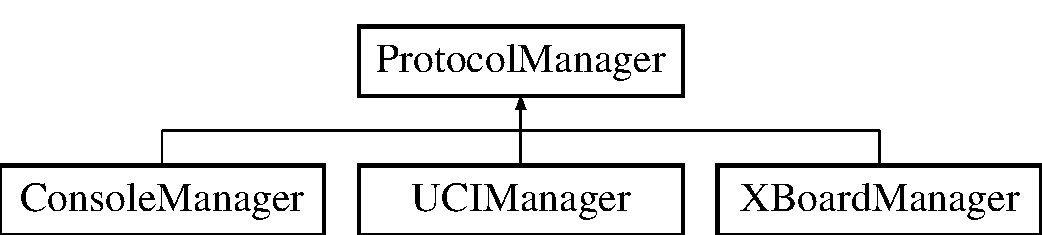
\includegraphics[height=2.000000cm]{classProtocolManager}
\end{center}
\end{figure}
\subsection*{Public Member Functions}
\begin{DoxyCompactItemize}
\item 
virtual void \mbox{\hyperlink{classProtocolManager_aa3ae25a03e2f070ea486fd9319715a6a}{loop}} ()=0
\begin{DoxyCompactList}\small\item\em Starts the protocol loop. \end{DoxyCompactList}\item 
virtual bool \mbox{\hyperlink{classProtocolManager_a1cab1bcb93ca3542821965e62ee59c33}{is\+Over}} ()
\begin{DoxyCompactList}\small\item\em Checks if the engine has recieved a stop signal from the G\+UI. \end{DoxyCompactList}\item 
virtual int32\+\_\+t \mbox{\hyperlink{classProtocolManager_a2ab274fd7510b28e7ac36405aebdbe82}{get\+Protocol}} ()=0
\begin{DoxyCompactList}\small\item\em Returns the protocol identifier for the current protocol. \end{DoxyCompactList}\end{DoxyCompactItemize}
\subsection*{Static Public Attributes}
\begin{DoxyCompactItemize}
\item 
\mbox{\Hypertarget{classProtocolManager_abda5da0d5f313a17757f56953cc9fb9c}\label{classProtocolManager_abda5da0d5f313a17757f56953cc9fb9c}} 
static constexpr int32\+\_\+t {\bfseries k\+U\+CI} = 0
\item 
\mbox{\Hypertarget{classProtocolManager_aae0d7c85f7908af043982e22b230164c}\label{classProtocolManager_aae0d7c85f7908af043982e22b230164c}} 
static constexpr int32\+\_\+t {\bfseries k\+X\+Board} = 1
\item 
\mbox{\Hypertarget{classProtocolManager_a5efa22d57690c47bc1e7aeaabe898ac8}\label{classProtocolManager_a5efa22d57690c47bc1e7aeaabe898ac8}} 
static constexpr int32\+\_\+t {\bfseries k\+Console} = 2
\end{DoxyCompactItemize}
\subsection*{Protected Attributes}
\begin{DoxyCompactItemize}
\item 
\mbox{\Hypertarget{classProtocolManager_ad8d2e4041601fb0fb0c51456641f2283}\label{classProtocolManager_ad8d2e4041601fb0fb0c51456641f2283}} 
\mbox{\hyperlink{classBoard}{Board}} {\bfseries pos}
\item 
\mbox{\Hypertarget{classProtocolManager_a1384f769e3bbb83e7876d0d8c21ce4fb}\label{classProtocolManager_a1384f769e3bbb83e7876d0d8c21ce4fb}} 
\mbox{\hyperlink{structSearchInfo}{Search\+Info}} {\bfseries info}
\item 
\mbox{\Hypertarget{classProtocolManager_af985b55fd4fb30eceae7f434c9c3ee05}\label{classProtocolManager_af985b55fd4fb30eceae7f434c9c3ee05}} 
\mbox{\hyperlink{classSearchAgent}{Search\+Agent}} {\bfseries sa}
\end{DoxyCompactItemize}


\subsection{Detailed Description}


Definition at line 15 of file protocol.\+h.



\subsection{Member Function Documentation}
\mbox{\Hypertarget{classProtocolManager_a2ab274fd7510b28e7ac36405aebdbe82}\label{classProtocolManager_a2ab274fd7510b28e7ac36405aebdbe82}} 
\index{Protocol\+Manager@{Protocol\+Manager}!get\+Protocol@{get\+Protocol}}
\index{get\+Protocol@{get\+Protocol}!Protocol\+Manager@{Protocol\+Manager}}
\subsubsection{\texorpdfstring{get\+Protocol()}{getProtocol()}}
{\footnotesize\ttfamily virtual int32\+\_\+t Protocol\+Manager\+::get\+Protocol (\begin{DoxyParamCaption}{ }\end{DoxyParamCaption})\hspace{0.3cm}{\ttfamily [pure virtual]}}



Returns the protocol identifier for the current protocol. 


\begin{DoxyParams}{Parameters}
{\em None} & \\
\hline
\end{DoxyParams}
\begin{DoxyReturn}{Returns}
The protocol identifier 
\end{DoxyReturn}


Implemented in \mbox{\hyperlink{classUCIManager_af85c53751a85a5cb624e10fb1f9962c7}{U\+C\+I\+Manager}}, \mbox{\hyperlink{classConsoleManager_a12c11521d46af302d6c7d79d3b8174b4}{Console\+Manager}}, and \mbox{\hyperlink{classXBoardManager_a388ebffa15fa11ee763f4144f01fbcaf}{X\+Board\+Manager}}.

\mbox{\Hypertarget{classProtocolManager_a1cab1bcb93ca3542821965e62ee59c33}\label{classProtocolManager_a1cab1bcb93ca3542821965e62ee59c33}} 
\index{Protocol\+Manager@{Protocol\+Manager}!is\+Over@{is\+Over}}
\index{is\+Over@{is\+Over}!Protocol\+Manager@{Protocol\+Manager}}
\subsubsection{\texorpdfstring{is\+Over()}{isOver()}}
{\footnotesize\ttfamily virtual bool Protocol\+Manager\+::is\+Over (\begin{DoxyParamCaption}{ }\end{DoxyParamCaption})\hspace{0.3cm}{\ttfamily [inline]}, {\ttfamily [virtual]}}



Checks if the engine has recieved a stop signal from the G\+UI. 


\begin{DoxyParams}{Parameters}
{\em None} & \\
\hline
\end{DoxyParams}
\begin{DoxyReturn}{Returns}
true if a stop command has been sent, false otherwise 
\end{DoxyReturn}


Definition at line 37 of file protocol.\+h.

\mbox{\Hypertarget{classProtocolManager_aa3ae25a03e2f070ea486fd9319715a6a}\label{classProtocolManager_aa3ae25a03e2f070ea486fd9319715a6a}} 
\index{Protocol\+Manager@{Protocol\+Manager}!loop@{loop}}
\index{loop@{loop}!Protocol\+Manager@{Protocol\+Manager}}
\subsubsection{\texorpdfstring{loop()}{loop()}}
{\footnotesize\ttfamily virtual void Protocol\+Manager\+::loop (\begin{DoxyParamCaption}{ }\end{DoxyParamCaption})\hspace{0.3cm}{\ttfamily [pure virtual]}}



Starts the protocol loop. 


\begin{DoxyParams}{Parameters}
{\em None} & \\
\hline
\end{DoxyParams}
\begin{DoxyReturn}{Returns}
None 
\end{DoxyReturn}


Implemented in \mbox{\hyperlink{classUCIManager_aa2fa2a352e6d58f00c8388da0d8541e1}{U\+C\+I\+Manager}}, \mbox{\hyperlink{classConsoleManager_a69261543a87cf7d3c7ec004c566145fd}{Console\+Manager}}, and \mbox{\hyperlink{classXBoardManager_a7d59ec1b3eaf1d140ad8f7cacd2ae956}{X\+Board\+Manager}}.



The documentation for this class was generated from the following file\+:\begin{DoxyCompactItemize}
\item 
/home/michael/\+Documents/\+Projects/\+C++/\+Chess-\/\+Engine/include/\mbox{\hyperlink{protocol_8h}{protocol.\+h}}\end{DoxyCompactItemize}

\hypertarget{classPvEntry}{}\section{Pv\+Entry Class Reference}
\label{classPvEntry}\index{Pv\+Entry@{Pv\+Entry}}


{\ttfamily \#include $<$pvtable.\+h$>$}

\subsection*{Public Member Functions}
\begin{DoxyCompactItemize}
\item 
\mbox{\Hypertarget{classPvEntry_afeeef31547873fa5fc9aa09ab4c4f06b}\label{classPvEntry_afeeef31547873fa5fc9aa09ab4c4f06b}} 
{\bfseries Pv\+Entry} (uint64\+\_\+t key, \mbox{\hyperlink{classMove}{Move}} \+\_\+move, int32\+\_\+t \+\_\+score, int32\+\_\+t \+\_\+depth, int32\+\_\+t \+\_\+flags) noexcept
\item 
\mbox{\Hypertarget{classPvEntry_ace4807fc22c58c833b65cf13ac09908a}\label{classPvEntry_ace4807fc22c58c833b65cf13ac09908a}} 
{\bfseries Pv\+Entry} (uint64\+\_\+t key, \mbox{\hyperlink{classMove}{Move}} move) noexcept
\item 
\mbox{\Hypertarget{classPvEntry_af33c5a8a15b3b08ba46255cd6b83b52e}\label{classPvEntry_af33c5a8a15b3b08ba46255cd6b83b52e}} 
{\bfseries Pv\+Entry} (const \mbox{\hyperlink{classPvEntry}{Pv\+Entry}} \&o) noexcept
\item 
\mbox{\Hypertarget{classPvEntry_ac55e594a47f0c00b0f32dcc41cb741ba}\label{classPvEntry_ac55e594a47f0c00b0f32dcc41cb741ba}} 
{\bfseries Pv\+Entry} (\mbox{\hyperlink{classPvEntry}{Pv\+Entry}} \&\&o) noexcept
\item 
\mbox{\Hypertarget{classPvEntry_aa435b3aa50a3820f911a38daece696ad}\label{classPvEntry_aa435b3aa50a3820f911a38daece696ad}} 
\mbox{\hyperlink{classPvEntry}{Pv\+Entry}} \& {\bfseries operator=} (const \mbox{\hyperlink{classPvEntry}{Pv\+Entry}} \&o) noexcept
\item 
\mbox{\Hypertarget{classPvEntry_aef1422ab13067d76d00d879ff053cd0b}\label{classPvEntry_aef1422ab13067d76d00d879ff053cd0b}} 
\mbox{\hyperlink{classPvEntry}{Pv\+Entry}} \& {\bfseries operator=} (\mbox{\hyperlink{classPvEntry}{Pv\+Entry}} \&\&o) noexcept
\end{DoxyCompactItemize}
\subsection*{Data Fields}
\begin{DoxyCompactItemize}
\item 
\mbox{\Hypertarget{classPvEntry_ab1e717bdabc6da4bf546d0b1af252091}\label{classPvEntry_ab1e717bdabc6da4bf546d0b1af252091}} 
uint64\+\_\+t {\bfseries pos\+\_\+key}
\item 
\mbox{\Hypertarget{classPvEntry_a6e6ab2e38db069902f7aeb2dae727a1e}\label{classPvEntry_a6e6ab2e38db069902f7aeb2dae727a1e}} 
\mbox{\hyperlink{classMove}{Move}} {\bfseries move}
\item 
\mbox{\Hypertarget{classPvEntry_a00a4547715d4b994bf2e889e7a4b29a9}\label{classPvEntry_a00a4547715d4b994bf2e889e7a4b29a9}} 
int32\+\_\+t {\bfseries score}
\item 
\mbox{\Hypertarget{classPvEntry_a75056e46bf9a3a8ed3955119fc83ace8}\label{classPvEntry_a75056e46bf9a3a8ed3955119fc83ace8}} 
int32\+\_\+t {\bfseries depth}
\item 
\mbox{\Hypertarget{classPvEntry_a90d1ef7b561954f7265af72e3cdd94be}\label{classPvEntry_a90d1ef7b561954f7265af72e3cdd94be}} 
int32\+\_\+t {\bfseries flags}
\end{DoxyCompactItemize}


\subsection{Detailed Description}
This class holds the cached info of our searches for use with the P\+V\+Table 

Definition at line 18 of file pvtable.\+h.



The documentation for this class was generated from the following files\+:\begin{DoxyCompactItemize}
\item 
include/\mbox{\hyperlink{pvtable_8h}{pvtable.\+h}}\item 
src/\mbox{\hyperlink{pvtable_8cc}{pvtable.\+cc}}\end{DoxyCompactItemize}

\hypertarget{classPvTable}{}\section{Pv\+Table Class Reference}
\label{classPvTable}\index{Pv\+Table@{Pv\+Table}}


{\ttfamily \#include $<$pvtable.\+h$>$}

\subsection*{Public Member Functions}
\begin{DoxyCompactItemize}
\item 
\mbox{\hyperlink{classMove}{Move}} \mbox{\hyperlink{classPvTable_affc22eb520f1e4c8fc30366e38af5868}{get}} (const \mbox{\hyperlink{classBoard}{Board}} \&pos) noexcept
\begin{DoxyCompactList}\small\item\em Get the best move previously found for this position. \end{DoxyCompactList}\item 
void \mbox{\hyperlink{classPvTable_aeb05a7085dcd5f16c35dbb30f152056a}{insert}} (const \mbox{\hyperlink{classBoard}{Board}} \&pos, const \mbox{\hyperlink{classMove}{Move}} \&move) noexcept
\begin{DoxyCompactList}\small\item\em Stashes the move associated with this position into the hash map. \end{DoxyCompactList}\item 
void \mbox{\hyperlink{classPvTable_ab26b0faf926e5c7de086f328ca1eaf79}{insert}} (const \mbox{\hyperlink{classBoard}{Board}} \&pos, const \mbox{\hyperlink{classMove}{Move}} \&move, int32\+\_\+t score, int32\+\_\+t depth, int32\+\_\+t flags) noexcept
\begin{DoxyCompactList}\small\item\em Stashes the move associated with this position into the hash map. \end{DoxyCompactList}\item 
int32\+\_\+t \mbox{\hyperlink{classPvTable_a6df38f01a626250eb8d1878d1fbb0029}{size}} () const noexcept
\begin{DoxyCompactList}\small\item\em Gets the number of entries in the transposition table. \end{DoxyCompactList}\item 
void \mbox{\hyperlink{classPvTable_a96b49a337793b2dc29d7f049ae54091f}{clear}} () noexcept
\begin{DoxyCompactList}\small\item\em Clears all entries in the transposition table. \end{DoxyCompactList}\item 
int32\+\_\+t \mbox{\hyperlink{classPvTable_a6e87189dbe8ce348782ad2423ac14b08}{get\+Pv\+Line}} (\mbox{\hyperlink{classBoard}{Board}} \&pos, const uint32\+\_\+t depth) noexcept
\begin{DoxyCompactList}\small\item\em Fills in the pv array with the searched pv moves and returns the length of the line. \end{DoxyCompactList}\item 
bool \mbox{\hyperlink{classPvTable_a0eb2e071414179f05f606ece66b8e0aa}{get\+Hash\+Entry}} (\mbox{\hyperlink{classBoard}{Board}} \&pos, \mbox{\hyperlink{classMove}{Move}} \&pv\+Move, int32\+\_\+t \&score, int32\+\_\+t alpha, int32\+\_\+t beta, int32\+\_\+t depth) noexcept
\begin{DoxyCompactList}\small\item\em Checks the alpha beta bounds and returns if a better, previously cached move is found. \end{DoxyCompactList}\end{DoxyCompactItemize}
\subsection*{Data Fields}
\begin{DoxyCompactItemize}
\item 
\mbox{\Hypertarget{classPvTable_aee04d36ed95071d6c553205e0b9de3e5}\label{classPvTable_aee04d36ed95071d6c553205e0b9de3e5}} 
std\+::vector$<$ \mbox{\hyperlink{classMove}{Move}} $>$ {\bfseries pv\+\_\+arr}
\end{DoxyCompactItemize}
\subsection*{Private Attributes}
\begin{DoxyCompactItemize}
\item 
\mbox{\Hypertarget{classPvTable_a10751ef66b0018b33e36623c24c44b91}\label{classPvTable_a10751ef66b0018b33e36623c24c44b91}} 
std\+::unordered\+\_\+map$<$ uint64\+\_\+t, \mbox{\hyperlink{classPvEntry}{Pv\+Entry}} $>$ {\bfseries pv\+\_\+table}
\end{DoxyCompactItemize}


\subsection{Detailed Description}
This class holds all info for a given position with the best move found. Serves as a cache to improve evaluation speed. Also called a transposition table. 

Definition at line 40 of file pvtable.\+h.



\subsection{Member Function Documentation}
\mbox{\Hypertarget{classPvTable_a96b49a337793b2dc29d7f049ae54091f}\label{classPvTable_a96b49a337793b2dc29d7f049ae54091f}} 
\index{Pv\+Table@{Pv\+Table}!clear@{clear}}
\index{clear@{clear}!Pv\+Table@{Pv\+Table}}
\subsubsection{\texorpdfstring{clear()}{clear()}}
{\footnotesize\ttfamily void Pv\+Table\+::clear (\begin{DoxyParamCaption}{ }\end{DoxyParamCaption})\hspace{0.3cm}{\ttfamily [noexcept]}}



Clears all entries in the transposition table. 


\begin{DoxyParams}{Parameters}
{\em None} & \\
\hline
\end{DoxyParams}
\begin{DoxyReturn}{Returns}
None 
\end{DoxyReturn}


Definition at line 89 of file pvtable.\+cc.

\mbox{\Hypertarget{classPvTable_affc22eb520f1e4c8fc30366e38af5868}\label{classPvTable_affc22eb520f1e4c8fc30366e38af5868}} 
\index{Pv\+Table@{Pv\+Table}!get@{get}}
\index{get@{get}!Pv\+Table@{Pv\+Table}}
\subsubsection{\texorpdfstring{get()}{get()}}
{\footnotesize\ttfamily \mbox{\hyperlink{classMove}{Move}} Pv\+Table\+::get (\begin{DoxyParamCaption}\item[{const \mbox{\hyperlink{classBoard}{Board}} \&}]{pos }\end{DoxyParamCaption})\hspace{0.3cm}{\ttfamily [noexcept]}}



Get the best move previously found for this position. 


\begin{DoxyParams}{Parameters}
{\em pos} & The current board state. \\
\hline
\end{DoxyParams}
\begin{DoxyReturn}{Returns}
The best move previously found for this position. 
\end{DoxyReturn}


Definition at line 58 of file pvtable.\+cc.

\mbox{\Hypertarget{classPvTable_a0eb2e071414179f05f606ece66b8e0aa}\label{classPvTable_a0eb2e071414179f05f606ece66b8e0aa}} 
\index{Pv\+Table@{Pv\+Table}!get\+Hash\+Entry@{get\+Hash\+Entry}}
\index{get\+Hash\+Entry@{get\+Hash\+Entry}!Pv\+Table@{Pv\+Table}}
\subsubsection{\texorpdfstring{get\+Hash\+Entry()}{getHashEntry()}}
{\footnotesize\ttfamily bool Pv\+Table\+::get\+Hash\+Entry (\begin{DoxyParamCaption}\item[{\mbox{\hyperlink{classBoard}{Board}} \&}]{pos,  }\item[{\mbox{\hyperlink{classMove}{Move}} \&}]{pv\+Move,  }\item[{int32\+\_\+t \&}]{score,  }\item[{int32\+\_\+t}]{alpha,  }\item[{int32\+\_\+t}]{beta,  }\item[{int32\+\_\+t}]{depth }\end{DoxyParamCaption})\hspace{0.3cm}{\ttfamily [noexcept]}}



Checks the alpha beta bounds and returns if a better, previously cached move is found. 


\begin{DoxyParams}{Parameters}
{\em pos} & The current board state. \\
\hline
{\em pv\+Move} & The move to store the found move in if found. \\
\hline
{\em score} & The score buffer to store the found score in if found \\
\hline
{\em alpha} & The alpha cutoff \\
\hline
{\em beta} & The beta cutoff \\
\hline
{\em depth} & The desired search depth \\
\hline
\end{DoxyParams}
\begin{DoxyReturn}{Returns}
true if the position has an applicable cached move. 
\end{DoxyReturn}


Definition at line 112 of file pvtable.\+cc.

\mbox{\Hypertarget{classPvTable_a6e87189dbe8ce348782ad2423ac14b08}\label{classPvTable_a6e87189dbe8ce348782ad2423ac14b08}} 
\index{Pv\+Table@{Pv\+Table}!get\+Pv\+Line@{get\+Pv\+Line}}
\index{get\+Pv\+Line@{get\+Pv\+Line}!Pv\+Table@{Pv\+Table}}
\subsubsection{\texorpdfstring{get\+Pv\+Line()}{getPvLine()}}
{\footnotesize\ttfamily int32\+\_\+t Pv\+Table\+::get\+Pv\+Line (\begin{DoxyParamCaption}\item[{\mbox{\hyperlink{classBoard}{Board}} \&}]{pos,  }\item[{const uint32\+\_\+t}]{depth }\end{DoxyParamCaption})\hspace{0.3cm}{\ttfamily [noexcept]}}



Fills in the pv array with the searched pv moves and returns the length of the line. 


\begin{DoxyParams}{Parameters}
{\em pos} & The current board state. \\
\hline
{\em depth} & The search depth. \\
\hline
\end{DoxyParams}
\begin{DoxyReturn}{Returns}
The number of moves in the Pv line 
\end{DoxyReturn}


Definition at line 94 of file pvtable.\+cc.

\mbox{\Hypertarget{classPvTable_aeb05a7085dcd5f16c35dbb30f152056a}\label{classPvTable_aeb05a7085dcd5f16c35dbb30f152056a}} 
\index{Pv\+Table@{Pv\+Table}!insert@{insert}}
\index{insert@{insert}!Pv\+Table@{Pv\+Table}}
\subsubsection{\texorpdfstring{insert()}{insert()}\hspace{0.1cm}{\footnotesize\ttfamily [1/2]}}
{\footnotesize\ttfamily void Pv\+Table\+::insert (\begin{DoxyParamCaption}\item[{const \mbox{\hyperlink{classBoard}{Board}} \&}]{pos,  }\item[{const \mbox{\hyperlink{classMove}{Move}} \&}]{move }\end{DoxyParamCaption})\hspace{0.3cm}{\ttfamily [noexcept]}}



Stashes the move associated with this position into the hash map. 


\begin{DoxyParams}{Parameters}
{\em pos} & The current board state. \\
\hline
{\em move} & The move to store for this position. \\
\hline
\end{DoxyParams}
\begin{DoxyReturn}{Returns}
None 
\end{DoxyReturn}


Definition at line 64 of file pvtable.\+cc.

\mbox{\Hypertarget{classPvTable_ab26b0faf926e5c7de086f328ca1eaf79}\label{classPvTable_ab26b0faf926e5c7de086f328ca1eaf79}} 
\index{Pv\+Table@{Pv\+Table}!insert@{insert}}
\index{insert@{insert}!Pv\+Table@{Pv\+Table}}
\subsubsection{\texorpdfstring{insert()}{insert()}\hspace{0.1cm}{\footnotesize\ttfamily [2/2]}}
{\footnotesize\ttfamily void Pv\+Table\+::insert (\begin{DoxyParamCaption}\item[{const \mbox{\hyperlink{classBoard}{Board}} \&}]{pos,  }\item[{const \mbox{\hyperlink{classMove}{Move}} \&}]{move,  }\item[{int32\+\_\+t}]{score,  }\item[{int32\+\_\+t}]{depth,  }\item[{int32\+\_\+t}]{flags }\end{DoxyParamCaption})\hspace{0.3cm}{\ttfamily [noexcept]}}



Stashes the move associated with this position into the hash map. 


\begin{DoxyParams}{Parameters}
{\em pos} & The current board state. \\
\hline
{\em move} & The move to store for this position. \\
\hline
{\em score} & The evaluation of this position. \\
\hline
{\em depth} & The depth that this position was previously searched to. \\
\hline
{\em flags} & The flags that are associated with the move. \\
\hline
\end{DoxyParams}
\begin{DoxyReturn}{Returns}
None 
\end{DoxyReturn}


Definition at line 70 of file pvtable.\+cc.

\mbox{\Hypertarget{classPvTable_a6df38f01a626250eb8d1878d1fbb0029}\label{classPvTable_a6df38f01a626250eb8d1878d1fbb0029}} 
\index{Pv\+Table@{Pv\+Table}!size@{size}}
\index{size@{size}!Pv\+Table@{Pv\+Table}}
\subsubsection{\texorpdfstring{size()}{size()}}
{\footnotesize\ttfamily int32\+\_\+t Pv\+Table\+::size (\begin{DoxyParamCaption}{ }\end{DoxyParamCaption}) const\hspace{0.3cm}{\ttfamily [noexcept]}}



Gets the number of entries in the transposition table. 


\begin{DoxyParams}{Parameters}
{\em None} & \\
\hline
\end{DoxyParams}
\begin{DoxyReturn}{Returns}
The number of entries in the transposition table. 
\end{DoxyReturn}


Definition at line 84 of file pvtable.\+cc.



The documentation for this class was generated from the following files\+:\begin{DoxyCompactItemize}
\item 
/home/michael/\+Documents/\+Projects/\+C++/\+Chess-\/\+Engine/include/\mbox{\hyperlink{pvtable_8h}{pvtable.\+h}}\item 
/home/michael/\+Documents/\+Projects/\+C++/\+Chess-\/\+Engine/src/\mbox{\hyperlink{pvtable_8cc}{pvtable.\+cc}}\end{DoxyCompactItemize}

\hypertarget{classSearchAgent}{}\section{Search\+Agent Class Reference}
\label{classSearchAgent}\index{Search\+Agent@{Search\+Agent}}


{\ttfamily \#include $<$search.\+h$>$}

\subsection*{Public Member Functions}
\begin{DoxyCompactItemize}
\item 
void \mbox{\hyperlink{classSearchAgent_a9bf258c0e75f45ab803cdcbde4d90fee}{search\+Position}} (\mbox{\hyperlink{classBoard}{Board}} \&pos, \mbox{\hyperlink{structSearchInfo}{Search\+Info}} \&info) noexcept
\begin{DoxyCompactList}\small\item\em Performs iterative deepening alpha-\/beta search on the position. \end{DoxyCompactList}\item 
bool \mbox{\hyperlink{classSearchAgent_ae345af56fed112c0c826653c07e2cd99}{is\+Game\+Over}} (\mbox{\hyperlink{classBoard}{Board}} \&pos) noexcept
\begin{DoxyCompactList}\small\item\em Checks if there is checkmate, stalemate, insufficient material, or threefold repetition. ~\newline
 \end{DoxyCompactList}\end{DoxyCompactItemize}
\subsection*{Data Fields}
\begin{DoxyCompactItemize}
\item 
\mbox{\Hypertarget{classSearchAgent_aaccc22d27a8b90a72608d3ff0bf4f758}\label{classSearchAgent_aaccc22d27a8b90a72608d3ff0bf4f758}} 
\mbox{\hyperlink{classEvaluator}{Evaluator}} {\bfseries eval}
\item 
\mbox{\Hypertarget{classSearchAgent_ac010d05e44c840531d4e9b05ec58b46a}\label{classSearchAgent_ac010d05e44c840531d4e9b05ec58b46a}} 
\mbox{\hyperlink{classPvTable}{Pv\+Table}} {\bfseries pv}
\end{DoxyCompactItemize}
\subsection*{Private Member Functions}
\begin{DoxyCompactItemize}
\item 
int32\+\_\+t \mbox{\hyperlink{classSearchAgent_acbc393afa5ab599c1bf3ffcd279b60a7}{is\+Repetition}} (const \mbox{\hyperlink{classBoard}{Board}} \&pos) noexcept
\begin{DoxyCompactList}\small\item\em Checks if the position has happened before. \end{DoxyCompactList}\item 
void \mbox{\hyperlink{classSearchAgent_aff45768956489f9696ff62c8db26db6b}{check\+Stop}} (\mbox{\hyperlink{structSearchInfo}{Search\+Info}} \&info)
\begin{DoxyCompactList}\small\item\em Checks if the time limit has been passed. \end{DoxyCompactList}\item 
void \mbox{\hyperlink{classSearchAgent_a5f8153e871a9030a537684323668a1cd}{clear\+For\+Search}} (\mbox{\hyperlink{classBoard}{Board}} \&pos, \mbox{\hyperlink{structSearchInfo}{Search\+Info}} \&info) noexcept
\begin{DoxyCompactList}\small\item\em Clears the board\textquotesingle{}s search\+\_\+hist and search\+\_\+killers vectors. \end{DoxyCompactList}\item 
int32\+\_\+t \mbox{\hyperlink{classSearchAgent_a276e7dc17f276cf7d1c5fe91218f55c2}{alpha\+Beta}} (int32\+\_\+t alpha, int32\+\_\+t beta, uint32\+\_\+t depth, \mbox{\hyperlink{classBoard}{Board}} \&pos, \mbox{\hyperlink{structSearchInfo}{Search\+Info}} \&info, bool do\+Null) noexcept
\begin{DoxyCompactList}\small\item\em Recursively performs the mini-\/max algorithm with alpha-\/beta pruning. If do\+Null is set, considers making a null move to improve search time. \end{DoxyCompactList}\item 
int32\+\_\+t \mbox{\hyperlink{classSearchAgent_a0a66b7b202216f6e794a963df3a83cb2}{quiescence\+Search}} (int32\+\_\+t alpha, int32\+\_\+t beta, \mbox{\hyperlink{classBoard}{Board}} \&pos, \mbox{\hyperlink{structSearchInfo}{Search\+Info}} \&info) noexcept
\begin{DoxyCompactList}\small\item\em Searches similarly to alpha-\/beta but only on capture moves. Used to avoid the horizon effect. ~\newline
 \end{DoxyCompactList}\item 
bool \mbox{\hyperlink{classSearchAgent_acaf7ae2df02a071a23e6db4fbbdc7d99}{three\+Fold\+Repetition}} (const \mbox{\hyperlink{classBoard}{Board}} \&pos) noexcept
\begin{DoxyCompactList}\small\item\em Checks if threefold repetition has occurred. \end{DoxyCompactList}\item 
bool \mbox{\hyperlink{classSearchAgent_a93b96a89b905ff786e520b23481ed0d7}{drawn\+Material}} (const \mbox{\hyperlink{classBoard}{Board}} \&pos) noexcept
\begin{DoxyCompactList}\small\item\em Checks if there is sufficient material to checkmate either side. \end{DoxyCompactList}\end{DoxyCompactItemize}
\subsection*{Static Private Attributes}
\begin{DoxyCompactItemize}
\item 
static constexpr uint32\+\_\+t \mbox{\hyperlink{classSearchAgent_ac040d91cab3fb103bce31d669d2bba47}{k\+Interval}} = 0x7\+FF
\end{DoxyCompactItemize}


\subsection{Detailed Description}
This class provides functions to search through the board state 

Definition at line 20 of file search.\+h.



\subsection{Member Function Documentation}
\mbox{\Hypertarget{classSearchAgent_a276e7dc17f276cf7d1c5fe91218f55c2}\label{classSearchAgent_a276e7dc17f276cf7d1c5fe91218f55c2}} 
\index{Search\+Agent@{Search\+Agent}!alpha\+Beta@{alpha\+Beta}}
\index{alpha\+Beta@{alpha\+Beta}!Search\+Agent@{Search\+Agent}}
\subsubsection{\texorpdfstring{alpha\+Beta()}{alphaBeta()}}
{\footnotesize\ttfamily int32\+\_\+t Search\+Agent\+::alpha\+Beta (\begin{DoxyParamCaption}\item[{int32\+\_\+t}]{alpha,  }\item[{int32\+\_\+t}]{beta,  }\item[{uint32\+\_\+t}]{depth,  }\item[{\mbox{\hyperlink{classBoard}{Board}} \&}]{pos,  }\item[{\mbox{\hyperlink{structSearchInfo}{Search\+Info}} \&}]{info,  }\item[{bool}]{do\+Null }\end{DoxyParamCaption})\hspace{0.3cm}{\ttfamily [private]}, {\ttfamily [noexcept]}}



Recursively performs the mini-\/max algorithm with alpha-\/beta pruning. If do\+Null is set, considers making a null move to improve search time. 


\begin{DoxyParams}{Parameters}
{\em pos} & The current board state. \\
\hline
{\em alpha} & The alpha cutoff \\
\hline
{\em beta} & The beta cutoff \\
\hline
{\em depth} & The current depth of the search \\
\hline
{\em pos} & The current board state \\
\hline
{\em info} & The engine\textquotesingle{}s search\+Info object \\
\hline
{\em do\+Null} & Null move flag \\
\hline
\end{DoxyParams}
\begin{DoxyReturn}{Returns}
The evaluation of the current position 
\end{DoxyReturn}


Definition at line 152 of file search.\+cc.

\mbox{\Hypertarget{classSearchAgent_aff45768956489f9696ff62c8db26db6b}\label{classSearchAgent_aff45768956489f9696ff62c8db26db6b}} 
\index{Search\+Agent@{Search\+Agent}!check\+Stop@{check\+Stop}}
\index{check\+Stop@{check\+Stop}!Search\+Agent@{Search\+Agent}}
\subsubsection{\texorpdfstring{check\+Stop()}{checkStop()}}
{\footnotesize\ttfamily void Search\+Agent\+::check\+Stop (\begin{DoxyParamCaption}\item[{\mbox{\hyperlink{structSearchInfo}{Search\+Info}} \&}]{info }\end{DoxyParamCaption})\hspace{0.3cm}{\ttfamily [private]}}



Checks if the time limit has been passed. 


\begin{DoxyParams}{Parameters}
{\em None} & \\
\hline
\end{DoxyParams}
\begin{DoxyReturn}{Returns}
None 
\end{DoxyReturn}


Definition at line 114 of file search.\+cc.

\mbox{\Hypertarget{classSearchAgent_a5f8153e871a9030a537684323668a1cd}\label{classSearchAgent_a5f8153e871a9030a537684323668a1cd}} 
\index{Search\+Agent@{Search\+Agent}!clear\+For\+Search@{clear\+For\+Search}}
\index{clear\+For\+Search@{clear\+For\+Search}!Search\+Agent@{Search\+Agent}}
\subsubsection{\texorpdfstring{clear\+For\+Search()}{clearForSearch()}}
{\footnotesize\ttfamily void Search\+Agent\+::clear\+For\+Search (\begin{DoxyParamCaption}\item[{\mbox{\hyperlink{classBoard}{Board}} \&}]{pos,  }\item[{\mbox{\hyperlink{structSearchInfo}{Search\+Info}} \&}]{info }\end{DoxyParamCaption})\hspace{0.3cm}{\ttfamily [private]}, {\ttfamily [noexcept]}}



Clears the board\textquotesingle{}s search\+\_\+hist and search\+\_\+killers vectors. 


\begin{DoxyParams}{Parameters}
{\em pos} & The current board state. \\
\hline
{\em info} & The engine\textquotesingle{}s search\+Info object. \\
\hline
\end{DoxyParams}
\begin{DoxyReturn}{Returns}
None 
\end{DoxyReturn}


Definition at line 126 of file search.\+cc.

\mbox{\Hypertarget{classSearchAgent_a93b96a89b905ff786e520b23481ed0d7}\label{classSearchAgent_a93b96a89b905ff786e520b23481ed0d7}} 
\index{Search\+Agent@{Search\+Agent}!drawn\+Material@{drawn\+Material}}
\index{drawn\+Material@{drawn\+Material}!Search\+Agent@{Search\+Agent}}
\subsubsection{\texorpdfstring{drawn\+Material()}{drawnMaterial()}}
{\footnotesize\ttfamily bool Search\+Agent\+::drawn\+Material (\begin{DoxyParamCaption}\item[{const \mbox{\hyperlink{classBoard}{Board}} \&}]{pos }\end{DoxyParamCaption})\hspace{0.3cm}{\ttfamily [private]}, {\ttfamily [noexcept]}}



Checks if there is sufficient material to checkmate either side. 


\begin{DoxyParams}{Parameters}
{\em pos} & The current board state \\
\hline
\end{DoxyParams}
\begin{DoxyReturn}{Returns}
true if there is sufficient material on either side to cause checkmate. 
\end{DoxyReturn}


Definition at line 34 of file search.\+cc.

\mbox{\Hypertarget{classSearchAgent_ae345af56fed112c0c826653c07e2cd99}\label{classSearchAgent_ae345af56fed112c0c826653c07e2cd99}} 
\index{Search\+Agent@{Search\+Agent}!is\+Game\+Over@{is\+Game\+Over}}
\index{is\+Game\+Over@{is\+Game\+Over}!Search\+Agent@{Search\+Agent}}
\subsubsection{\texorpdfstring{is\+Game\+Over()}{isGameOver()}}
{\footnotesize\ttfamily bool Search\+Agent\+::is\+Game\+Over (\begin{DoxyParamCaption}\item[{\mbox{\hyperlink{classBoard}{Board}} \&}]{pos }\end{DoxyParamCaption})\hspace{0.3cm}{\ttfamily [noexcept]}}



Checks if there is checkmate, stalemate, insufficient material, or threefold repetition. ~\newline
 


\begin{DoxyParams}{Parameters}
{\em pos} & The current board state \\
\hline
\end{DoxyParams}
\begin{DoxyReturn}{Returns}
true if the game has concluded in one way or other, false otherwise 
\end{DoxyReturn}


Definition at line 59 of file search.\+cc.

\mbox{\Hypertarget{classSearchAgent_acbc393afa5ab599c1bf3ffcd279b60a7}\label{classSearchAgent_acbc393afa5ab599c1bf3ffcd279b60a7}} 
\index{Search\+Agent@{Search\+Agent}!is\+Repetition@{is\+Repetition}}
\index{is\+Repetition@{is\+Repetition}!Search\+Agent@{Search\+Agent}}
\subsubsection{\texorpdfstring{is\+Repetition()}{isRepetition()}}
{\footnotesize\ttfamily int32\+\_\+t Search\+Agent\+::is\+Repetition (\begin{DoxyParamCaption}\item[{const \mbox{\hyperlink{classBoard}{Board}} \&}]{pos }\end{DoxyParamCaption})\hspace{0.3cm}{\ttfamily [private]}, {\ttfamily [noexcept]}}



Checks if the position has happened before. 


\begin{DoxyParams}{Parameters}
{\em pos} & The current board state. \\
\hline
\end{DoxyParams}
\begin{DoxyReturn}{Returns}
true if the current position has happened before, false otherwise 
\end{DoxyReturn}


Definition at line 47 of file search.\+cc.

\mbox{\Hypertarget{classSearchAgent_a0a66b7b202216f6e794a963df3a83cb2}\label{classSearchAgent_a0a66b7b202216f6e794a963df3a83cb2}} 
\index{Search\+Agent@{Search\+Agent}!quiescence\+Search@{quiescence\+Search}}
\index{quiescence\+Search@{quiescence\+Search}!Search\+Agent@{Search\+Agent}}
\subsubsection{\texorpdfstring{quiescence\+Search()}{quiescenceSearch()}}
{\footnotesize\ttfamily int32\+\_\+t Search\+Agent\+::quiescence\+Search (\begin{DoxyParamCaption}\item[{int32\+\_\+t}]{alpha,  }\item[{int32\+\_\+t}]{beta,  }\item[{\mbox{\hyperlink{classBoard}{Board}} \&}]{pos,  }\item[{\mbox{\hyperlink{structSearchInfo}{Search\+Info}} \&}]{info }\end{DoxyParamCaption})\hspace{0.3cm}{\ttfamily [private]}, {\ttfamily [noexcept]}}



Searches similarly to alpha-\/beta but only on capture moves. Used to avoid the horizon effect. ~\newline
 


\begin{DoxyParams}{Parameters}
{\em alpha} & The alpha cutoff \\
\hline
{\em beta} & The beta cutoff \\
\hline
{\em pos} & The current board state \\
\hline
{\em info} & The engine\textquotesingle{}s search\+Info object \\
\hline
\end{DoxyParams}
\begin{DoxyReturn}{Returns}
The evaluation of the current position 
\end{DoxyReturn}


Definition at line 303 of file search.\+cc.

\mbox{\Hypertarget{classSearchAgent_a9bf258c0e75f45ab803cdcbde4d90fee}\label{classSearchAgent_a9bf258c0e75f45ab803cdcbde4d90fee}} 
\index{Search\+Agent@{Search\+Agent}!search\+Position@{search\+Position}}
\index{search\+Position@{search\+Position}!Search\+Agent@{Search\+Agent}}
\subsubsection{\texorpdfstring{search\+Position()}{searchPosition()}}
{\footnotesize\ttfamily void Search\+Agent\+::search\+Position (\begin{DoxyParamCaption}\item[{\mbox{\hyperlink{classBoard}{Board}} \&}]{pos,  }\item[{\mbox{\hyperlink{structSearchInfo}{Search\+Info}} \&}]{info }\end{DoxyParamCaption})\hspace{0.3cm}{\ttfamily [noexcept]}}



Performs iterative deepening alpha-\/beta search on the position. 


\begin{DoxyParams}{Parameters}
{\em pos} & The current board state \\
\hline
{\em info} & The engine\textquotesingle{}s search\+Info object \\
\hline
\end{DoxyParams}
\begin{DoxyReturn}{Returns}
None 
\end{DoxyReturn}


Definition at line 367 of file search.\+cc.

\mbox{\Hypertarget{classSearchAgent_acaf7ae2df02a071a23e6db4fbbdc7d99}\label{classSearchAgent_acaf7ae2df02a071a23e6db4fbbdc7d99}} 
\index{Search\+Agent@{Search\+Agent}!three\+Fold\+Repetition@{three\+Fold\+Repetition}}
\index{three\+Fold\+Repetition@{three\+Fold\+Repetition}!Search\+Agent@{Search\+Agent}}
\subsubsection{\texorpdfstring{three\+Fold\+Repetition()}{threeFoldRepetition()}}
{\footnotesize\ttfamily bool Search\+Agent\+::three\+Fold\+Repetition (\begin{DoxyParamCaption}\item[{const \mbox{\hyperlink{classBoard}{Board}} \&}]{pos }\end{DoxyParamCaption})\hspace{0.3cm}{\ttfamily [private]}, {\ttfamily [noexcept]}}



Checks if threefold repetition has occurred. 


\begin{DoxyParams}{Parameters}
{\em pos} & The current board state \\
\hline
\end{DoxyParams}
\begin{DoxyReturn}{Returns}
true if threefold repetition has occurred, false otherwise. 
\end{DoxyReturn}


Definition at line 21 of file search.\+cc.



\subsection{Field Documentation}
\mbox{\Hypertarget{classSearchAgent_ac040d91cab3fb103bce31d669d2bba47}\label{classSearchAgent_ac040d91cab3fb103bce31d669d2bba47}} 
\index{Search\+Agent@{Search\+Agent}!k\+Interval@{k\+Interval}}
\index{k\+Interval@{k\+Interval}!Search\+Agent@{Search\+Agent}}
\subsubsection{\texorpdfstring{k\+Interval}{kInterval}}
{\footnotesize\ttfamily constexpr uint32\+\_\+t Search\+Agent\+::k\+Interval = 0x7\+FF\hspace{0.3cm}{\ttfamily [static]}, {\ttfamily [private]}}

Bitmask to check search flags every 2048 positions 

Definition at line 26 of file search.\+h.



The documentation for this class was generated from the following files\+:\begin{DoxyCompactItemize}
\item 
/home/michael/\+Documents/\+Projects/\+C++/\+Chess-\/\+Engine/include/\mbox{\hyperlink{search_8h}{search.\+h}}\item 
/home/michael/\+Documents/\+Projects/\+C++/\+Chess-\/\+Engine/src/\mbox{\hyperlink{search_8cc}{search.\+cc}}\end{DoxyCompactItemize}

\hypertarget{structSearchInfo}{}\section{Search\+Info Struct Reference}
\label{structSearchInfo}\index{Search\+Info@{Search\+Info}}
\subsection*{Data Fields}
\begin{DoxyCompactItemize}
\item 
\mbox{\Hypertarget{structSearchInfo_a6941b86fe82fed27ccb215058b1ebaca}\label{structSearchInfo_a6941b86fe82fed27ccb215058b1ebaca}} 
uint64\+\_\+t {\bfseries start\+Time}
\item 
\mbox{\Hypertarget{structSearchInfo_a63783b4e0f5ce8ca6c879602f13f059c}\label{structSearchInfo_a63783b4e0f5ce8ca6c879602f13f059c}} 
uint64\+\_\+t {\bfseries stop\+Time}
\item 
\mbox{\Hypertarget{structSearchInfo_a59ba0ab42e54ce6a7802b9539cc83dd2}\label{structSearchInfo_a59ba0ab42e54ce6a7802b9539cc83dd2}} 
bool {\bfseries time\+Limit}
\item 
\mbox{\Hypertarget{structSearchInfo_af38c629d4cf4f3679011e5a29a52c86e}\label{structSearchInfo_af38c629d4cf4f3679011e5a29a52c86e}} 
uint32\+\_\+t {\bfseries depth}
\item 
\mbox{\Hypertarget{structSearchInfo_a1086806af79fa252ac177bc758298df8}\label{structSearchInfo_a1086806af79fa252ac177bc758298df8}} 
uint32\+\_\+t {\bfseries depth\+Limit}
\item 
\mbox{\Hypertarget{structSearchInfo_a06e212fc443a1d9544534a06640c8d5f}\label{structSearchInfo_a06e212fc443a1d9544534a06640c8d5f}} 
uint32\+\_\+t {\bfseries nodes}
\item 
\mbox{\Hypertarget{structSearchInfo_ae86581f2a80db0d11ff3f9e4c3f402ec}\label{structSearchInfo_ae86581f2a80db0d11ff3f9e4c3f402ec}} 
uint32\+\_\+t {\bfseries moves\+Left}
\item 
\mbox{\Hypertarget{structSearchInfo_afbf237162fbae5d667857d6edff2db8f}\label{structSearchInfo_afbf237162fbae5d667857d6edff2db8f}} 
bool {\bfseries infinite}
\item 
\mbox{\Hypertarget{structSearchInfo_ae1437efa9afa50befedfa2b517e438c6}\label{structSearchInfo_ae1437efa9afa50befedfa2b517e438c6}} 
bool {\bfseries quit}
\item 
\mbox{\Hypertarget{structSearchInfo_afd8a3398b992f2fb4aad70bc0016c9de}\label{structSearchInfo_afd8a3398b992f2fb4aad70bc0016c9de}} 
bool {\bfseries stopped}
\item 
\mbox{\Hypertarget{structSearchInfo_aaf93702aef0d1eb5754b0b1e35574631}\label{structSearchInfo_aaf93702aef0d1eb5754b0b1e35574631}} 
float {\bfseries fh}
\item 
\mbox{\Hypertarget{structSearchInfo_a0a6e9abcf065a2c0f7245f47db569abe}\label{structSearchInfo_a0a6e9abcf065a2c0f7245f47db569abe}} 
float {\bfseries fhf}
\item 
\mbox{\Hypertarget{structSearchInfo_ac3f008988acc4aa6fceb4e120a9471cb}\label{structSearchInfo_ac3f008988acc4aa6fceb4e120a9471cb}} 
int32\+\_\+t {\bfseries protocol}
\item 
\mbox{\Hypertarget{structSearchInfo_a2cc71d1a67abdc16091a32f269685032}\label{structSearchInfo_a2cc71d1a67abdc16091a32f269685032}} 
bool {\bfseries do\+Print}
\end{DoxyCompactItemize}


\subsection{Detailed Description}


Definition at line 11 of file searchinfo.\+h.



The documentation for this struct was generated from the following file\+:\begin{DoxyCompactItemize}
\item 
include/\mbox{\hyperlink{searchinfo_8h}{searchinfo.\+h}}\end{DoxyCompactItemize}

\hypertarget{classStopwatch}{}\section{Stopwatch Class Reference}
\label{classStopwatch}\index{Stopwatch@{Stopwatch}}
\subsection*{Public Member Functions}
\begin{DoxyCompactItemize}
\item 
void \mbox{\hyperlink{classStopwatch_aff8757dda8e913cc671eb3baeb662109}{start}} () noexcept
\begin{DoxyCompactList}\small\item\em Starts the internal timer. \end{DoxyCompactList}\item 
float \mbox{\hyperlink{classStopwatch_ae614c46daae8d773f15d7ff603245cd0}{stop}} () noexcept
\begin{DoxyCompactList}\small\item\em Stops the internal timer and returns the time elapsed. \end{DoxyCompactList}\end{DoxyCompactItemize}
\subsection*{Static Public Member Functions}
\begin{DoxyCompactItemize}
\item 
static uint64\+\_\+t \mbox{\hyperlink{classStopwatch_a789c42b276146b4d043fac2e30684d7c}{get\+Time\+In\+Milli}} () noexcept
\begin{DoxyCompactList}\small\item\em Get the time since the epoch in milliseconds. \end{DoxyCompactList}\end{DoxyCompactItemize}
\subsection*{Static Public Attributes}
\begin{DoxyCompactItemize}
\item 
\mbox{\Hypertarget{classStopwatch_a9d3511a4c1fb3544757883f0ffc6f140}\label{classStopwatch_a9d3511a4c1fb3544757883f0ffc6f140}} 
static constexpr int32\+\_\+t {\bfseries k\+Milli\+Per\+Second} = 1000
\item 
\mbox{\Hypertarget{classStopwatch_a2603fc92466f39b1ac12718ac3d052e8}\label{classStopwatch_a2603fc92466f39b1ac12718ac3d052e8}} 
static constexpr int32\+\_\+t {\bfseries k\+Seconds\+Per\+Minute} = 60
\end{DoxyCompactItemize}
\subsection*{Private Types}
\begin{DoxyCompactItemize}
\item 
\mbox{\Hypertarget{classStopwatch_aa9ff69ca66fa3a4dde86ba27e03bb7b8}\label{classStopwatch_aa9ff69ca66fa3a4dde86ba27e03bb7b8}} 
typedef std\+::chrono\+::high\+\_\+resolution\+\_\+clock {\bfseries Time}
\item 
\mbox{\Hypertarget{classStopwatch_ac126d5ce9b6c280a79630bb65e4df83a}\label{classStopwatch_ac126d5ce9b6c280a79630bb65e4df83a}} 
typedef std\+::chrono\+::milliseconds {\bfseries ms}
\end{DoxyCompactItemize}
\subsection*{Private Attributes}
\begin{DoxyCompactItemize}
\item 
\mbox{\Hypertarget{classStopwatch_a9252f7329528193968d74bd3502f3bba}\label{classStopwatch_a9252f7329528193968d74bd3502f3bba}} 
Time\+::time\+\_\+point {\bfseries start\+\_\+time}
\end{DoxyCompactItemize}


\subsection{Detailed Description}


Definition at line 13 of file stopwatch.\+h.



\subsection{Member Function Documentation}
\mbox{\Hypertarget{classStopwatch_a789c42b276146b4d043fac2e30684d7c}\label{classStopwatch_a789c42b276146b4d043fac2e30684d7c}} 
\index{Stopwatch@{Stopwatch}!get\+Time\+In\+Milli@{get\+Time\+In\+Milli}}
\index{get\+Time\+In\+Milli@{get\+Time\+In\+Milli}!Stopwatch@{Stopwatch}}
\subsubsection{\texorpdfstring{get\+Time\+In\+Milli()}{getTimeInMilli()}}
{\footnotesize\ttfamily uint64\+\_\+t Stopwatch\+::get\+Time\+In\+Milli (\begin{DoxyParamCaption}{ }\end{DoxyParamCaption})\hspace{0.3cm}{\ttfamily [static]}, {\ttfamily [noexcept]}}



Get the time since the epoch in milliseconds. 


\begin{DoxyParams}{Parameters}
{\em None} & \\
\hline
\end{DoxyParams}
\begin{DoxyReturn}{Returns}
Get the time since the epoch in milliseconds 
\end{DoxyReturn}


Definition at line 28 of file stopwatch.\+cc.

\mbox{\Hypertarget{classStopwatch_aff8757dda8e913cc671eb3baeb662109}\label{classStopwatch_aff8757dda8e913cc671eb3baeb662109}} 
\index{Stopwatch@{Stopwatch}!start@{start}}
\index{start@{start}!Stopwatch@{Stopwatch}}
\subsubsection{\texorpdfstring{start()}{start()}}
{\footnotesize\ttfamily void Stopwatch\+::start (\begin{DoxyParamCaption}{ }\end{DoxyParamCaption})\hspace{0.3cm}{\ttfamily [noexcept]}}



Starts the internal timer. 


\begin{DoxyParams}{Parameters}
{\em None} & \\
\hline
\end{DoxyParams}
\begin{DoxyReturn}{Returns}
None 
\end{DoxyReturn}


Definition at line 16 of file stopwatch.\+cc.

\mbox{\Hypertarget{classStopwatch_ae614c46daae8d773f15d7ff603245cd0}\label{classStopwatch_ae614c46daae8d773f15d7ff603245cd0}} 
\index{Stopwatch@{Stopwatch}!stop@{stop}}
\index{stop@{stop}!Stopwatch@{Stopwatch}}
\subsubsection{\texorpdfstring{stop()}{stop()}}
{\footnotesize\ttfamily float Stopwatch\+::stop (\begin{DoxyParamCaption}{ }\end{DoxyParamCaption})\hspace{0.3cm}{\ttfamily [noexcept]}}



Stops the internal timer and returns the time elapsed. 


\begin{DoxyParams}{Parameters}
{\em None} & \\
\hline
\end{DoxyParams}
\begin{DoxyReturn}{Returns}
The time elapsed since \mbox{\hyperlink{classStopwatch_aff8757dda8e913cc671eb3baeb662109}{start()}} was called in milliseconds. 
\end{DoxyReturn}


Definition at line 21 of file stopwatch.\+cc.



The documentation for this class was generated from the following files\+:\begin{DoxyCompactItemize}
\item 
include/\mbox{\hyperlink{stopwatch_8h}{stopwatch.\+h}}\item 
src/\mbox{\hyperlink{stopwatch_8cc}{stopwatch.\+cc}}\end{DoxyCompactItemize}

\hypertarget{classUCIManager}{}\section{U\+C\+I\+Manager Class Reference}
\label{classUCIManager}\index{U\+C\+I\+Manager@{U\+C\+I\+Manager}}


{\ttfamily \#include $<$uci.\+h$>$}

Inheritance diagram for U\+C\+I\+Manager\+:\begin{figure}[H]
\begin{center}
\leavevmode
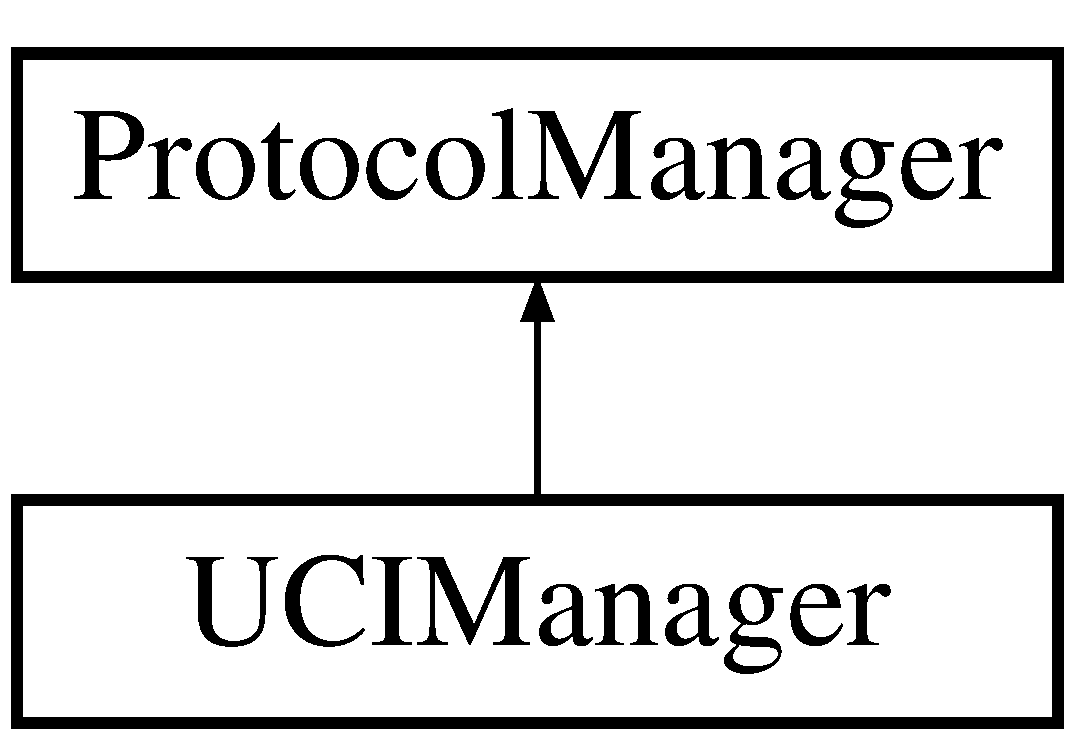
\includegraphics[height=2.000000cm]{classUCIManager}
\end{center}
\end{figure}
\subsection*{Public Member Functions}
\begin{DoxyCompactItemize}
\item 
\mbox{\Hypertarget{classUCIManager_aa8959f05532509ccee25ef91e3edde63}\label{classUCIManager_aa8959f05532509ccee25ef91e3edde63}} 
void {\bfseries parse\+Go\+Cmd} (const std\+::string \&cmd)
\item 
\mbox{\Hypertarget{classUCIManager_a71a9473ca9e8ba6486c77326dace417e}\label{classUCIManager_a71a9473ca9e8ba6486c77326dace417e}} 
void {\bfseries parse\+Position} (const std\+::string \&input)
\item 
void \mbox{\hyperlink{classUCIManager_aa2fa2a352e6d58f00c8388da0d8541e1}{loop}} () override
\begin{DoxyCompactList}\small\item\em Starts the protocol loop. \end{DoxyCompactList}\item 
int32\+\_\+t \mbox{\hyperlink{classUCIManager_af85c53751a85a5cb624e10fb1f9962c7}{get\+Protocol}} () override
\begin{DoxyCompactList}\small\item\em Returns the protocol identifier for the current protocol. \end{DoxyCompactList}\end{DoxyCompactItemize}
\subsection*{Additional Inherited Members}


\subsection{Detailed Description}
See \mbox{\hyperlink{classProtocolManager}{Protocol\+Manager}} documentation 

Definition at line 15 of file uci.\+h.



\subsection{Member Function Documentation}
\mbox{\Hypertarget{classUCIManager_af85c53751a85a5cb624e10fb1f9962c7}\label{classUCIManager_af85c53751a85a5cb624e10fb1f9962c7}} 
\index{U\+C\+I\+Manager@{U\+C\+I\+Manager}!get\+Protocol@{get\+Protocol}}
\index{get\+Protocol@{get\+Protocol}!U\+C\+I\+Manager@{U\+C\+I\+Manager}}
\subsubsection{\texorpdfstring{get\+Protocol()}{getProtocol()}}
{\footnotesize\ttfamily int32\+\_\+t U\+C\+I\+Manager\+::get\+Protocol (\begin{DoxyParamCaption}{ }\end{DoxyParamCaption})\hspace{0.3cm}{\ttfamily [override]}, {\ttfamily [virtual]}}



Returns the protocol identifier for the current protocol. 


\begin{DoxyParams}{Parameters}
{\em None} & \\
\hline
\end{DoxyParams}
\begin{DoxyReturn}{Returns}
The protocol identifier 
\end{DoxyReturn}


Implements \mbox{\hyperlink{classProtocolManager_a2ab274fd7510b28e7ac36405aebdbe82}{Protocol\+Manager}}.



Definition at line 203 of file uci.\+cc.

\mbox{\Hypertarget{classUCIManager_aa2fa2a352e6d58f00c8388da0d8541e1}\label{classUCIManager_aa2fa2a352e6d58f00c8388da0d8541e1}} 
\index{U\+C\+I\+Manager@{U\+C\+I\+Manager}!loop@{loop}}
\index{loop@{loop}!U\+C\+I\+Manager@{U\+C\+I\+Manager}}
\subsubsection{\texorpdfstring{loop()}{loop()}}
{\footnotesize\ttfamily void U\+C\+I\+Manager\+::loop (\begin{DoxyParamCaption}{ }\end{DoxyParamCaption})\hspace{0.3cm}{\ttfamily [override]}, {\ttfamily [virtual]}}



Starts the protocol loop. 


\begin{DoxyParams}{Parameters}
{\em None} & \\
\hline
\end{DoxyParams}
\begin{DoxyReturn}{Returns}
None 
\end{DoxyReturn}


Implements \mbox{\hyperlink{classProtocolManager_aa3ae25a03e2f070ea486fd9319715a6a}{Protocol\+Manager}}.



Definition at line 134 of file uci.\+cc.



The documentation for this class was generated from the following files\+:\begin{DoxyCompactItemize}
\item 
/home/michael/\+Documents/\+Projects/\+C++/\+Chess-\/\+Engine/include/\mbox{\hyperlink{uci_8h}{uci.\+h}}\item 
/home/michael/\+Documents/\+Projects/\+C++/\+Chess-\/\+Engine/src/\mbox{\hyperlink{uci_8cc}{uci.\+cc}}\end{DoxyCompactItemize}

\hypertarget{classUndoMove}{}\section{Undo\+Move Class Reference}
\label{classUndoMove}\index{Undo\+Move@{Undo\+Move}}


This class stores info needed to undo a move that was made.  




{\ttfamily \#include $<$move.\+h$>$}

\subsection*{Public Member Functions}
\begin{DoxyCompactItemize}
\item 
\mbox{\Hypertarget{classUndoMove_a3de052beeee8272912fba95e1f097c15}\label{classUndoMove_a3de052beeee8272912fba95e1f097c15}} 
{\bfseries Undo\+Move} (int32\+\_\+t \+\_\+move, const \mbox{\hyperlink{classBoard}{Board}} \&pos)
\end{DoxyCompactItemize}
\subsection*{Data Fields}
\begin{DoxyCompactItemize}
\item 
\mbox{\Hypertarget{classUndoMove_a829f8e9963dac72b42c166ab62cc9bca}\label{classUndoMove_a829f8e9963dac72b42c166ab62cc9bca}} 
int32\+\_\+t {\bfseries move}
\item 
\mbox{\Hypertarget{classUndoMove_ae1ea12b372aff6f9636c2c185f7ec1c1}\label{classUndoMove_ae1ea12b372aff6f9636c2c185f7ec1c1}} 
int32\+\_\+t {\bfseries castle\+\_\+perm}
\item 
\mbox{\Hypertarget{classUndoMove_a801d7c221484ce9e9d70c16c8d0a5749}\label{classUndoMove_a801d7c221484ce9e9d70c16c8d0a5749}} 
int32\+\_\+t {\bfseries en\+\_\+pas}
\item 
\mbox{\Hypertarget{classUndoMove_ac4e428deda8affe8713ab5f9fb0d9d5b}\label{classUndoMove_ac4e428deda8affe8713ab5f9fb0d9d5b}} 
int32\+\_\+t {\bfseries fifty\+\_\+move}
\item 
\mbox{\Hypertarget{classUndoMove_ae03b245ae0d4c790ad8c7077a837ec14}\label{classUndoMove_ae03b245ae0d4c790ad8c7077a837ec14}} 
uint64\+\_\+t {\bfseries pos\+\_\+key}
\end{DoxyCompactItemize}


\subsection{Detailed Description}
This class stores info needed to undo a move that was made. 

Definition at line 17 of file move.\+h.



The documentation for this class was generated from the following files\+:\begin{DoxyCompactItemize}
\item 
include/\mbox{\hyperlink{move_8h}{move.\+h}}\item 
src/\mbox{\hyperlink{move_8cc}{move.\+cc}}\end{DoxyCompactItemize}

\hypertarget{classXBoardManager}{}\section{X\+Board\+Manager Class Reference}
\label{classXBoardManager}\index{X\+Board\+Manager@{X\+Board\+Manager}}


{\ttfamily \#include $<$xboard.\+h$>$}

Inheritance diagram for X\+Board\+Manager\+:\begin{figure}[H]
\begin{center}
\leavevmode
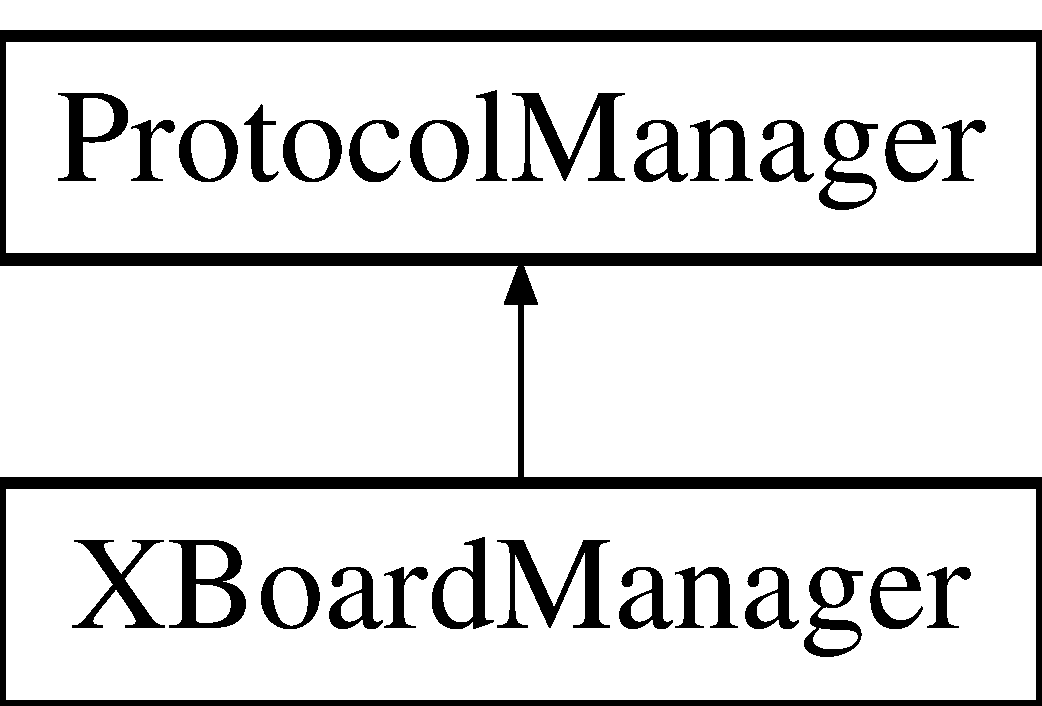
\includegraphics[height=2.000000cm]{classXBoardManager}
\end{center}
\end{figure}
\subsection*{Public Member Functions}
\begin{DoxyCompactItemize}
\item 
void \mbox{\hyperlink{classXBoardManager_a7d59ec1b3eaf1d140ad8f7cacd2ae956}{loop}} () override
\begin{DoxyCompactList}\small\item\em Starts the protocol loop. \end{DoxyCompactList}\item 
int32\+\_\+t \mbox{\hyperlink{classXBoardManager_a388ebffa15fa11ee763f4144f01fbcaf}{get\+Protocol}} () override
\begin{DoxyCompactList}\small\item\em Returns the protocol identifier for the current protocol. \end{DoxyCompactList}\end{DoxyCompactItemize}
\subsection*{Additional Inherited Members}


\subsection{Detailed Description}
See \mbox{\hyperlink{classProtocolManager}{Protocol\+Manager}} documentation 

Definition at line 14 of file xboard.\+h.



\subsection{Member Function Documentation}
\mbox{\Hypertarget{classXBoardManager_a388ebffa15fa11ee763f4144f01fbcaf}\label{classXBoardManager_a388ebffa15fa11ee763f4144f01fbcaf}} 
\index{X\+Board\+Manager@{X\+Board\+Manager}!get\+Protocol@{get\+Protocol}}
\index{get\+Protocol@{get\+Protocol}!X\+Board\+Manager@{X\+Board\+Manager}}
\subsubsection{\texorpdfstring{get\+Protocol()}{getProtocol()}}
{\footnotesize\ttfamily int32\+\_\+t X\+Board\+Manager\+::get\+Protocol (\begin{DoxyParamCaption}{ }\end{DoxyParamCaption})\hspace{0.3cm}{\ttfamily [override]}, {\ttfamily [virtual]}}



Returns the protocol identifier for the current protocol. 


\begin{DoxyParams}{Parameters}
{\em None} & \\
\hline
\end{DoxyParams}
\begin{DoxyReturn}{Returns}
The protocol identifier 
\end{DoxyReturn}


Implements \mbox{\hyperlink{classProtocolManager_a2ab274fd7510b28e7ac36405aebdbe82}{Protocol\+Manager}}.



Definition at line 163 of file xboard.\+cc.

\mbox{\Hypertarget{classXBoardManager_a7d59ec1b3eaf1d140ad8f7cacd2ae956}\label{classXBoardManager_a7d59ec1b3eaf1d140ad8f7cacd2ae956}} 
\index{X\+Board\+Manager@{X\+Board\+Manager}!loop@{loop}}
\index{loop@{loop}!X\+Board\+Manager@{X\+Board\+Manager}}
\subsubsection{\texorpdfstring{loop()}{loop()}}
{\footnotesize\ttfamily void X\+Board\+Manager\+::loop (\begin{DoxyParamCaption}{ }\end{DoxyParamCaption})\hspace{0.3cm}{\ttfamily [override]}, {\ttfamily [virtual]}}



Starts the protocol loop. 


\begin{DoxyParams}{Parameters}
{\em None} & \\
\hline
\end{DoxyParams}
\begin{DoxyReturn}{Returns}
None 
\end{DoxyReturn}


Implements \mbox{\hyperlink{classProtocolManager_aa3ae25a03e2f070ea486fd9319715a6a}{Protocol\+Manager}}.



Definition at line 19 of file xboard.\+cc.



The documentation for this class was generated from the following files\+:\begin{DoxyCompactItemize}
\item 
include/\mbox{\hyperlink{xboard_8h}{xboard.\+h}}\item 
src/\mbox{\hyperlink{xboard_8cc}{xboard.\+cc}}\end{DoxyCompactItemize}

\chapter{File Documentation}
\hypertarget{bitboard_8h}{}\section{include/bitboard.h File Reference}
\label{bitboard_8h}\index{include/bitboard.\+h@{include/bitboard.\+h}}


Contains declarations of functions that manipulate bitboards.  


{\ttfamily \#include \char`\"{}defs.\+h\char`\"{}}\newline
\subsection*{Functions}
\begin{DoxyCompactItemize}
\item 
int \mbox{\hyperlink{bitboard_8h_a64427fd1eee98a36ce930f3a236d1274}{B\+B\+::pop\+Bit}} (uint64\+\_\+t \&bb) noexcept
\begin{DoxyCompactList}\small\item\em Sets the highest order 1 bit to 0. \end{DoxyCompactList}\item 
int \mbox{\hyperlink{bitboard_8h_ae9ac6d5ba9f117b648a13a99374e13b9}{B\+B\+::count\+Bits}} (uint64\+\_\+t bb) noexcept
\begin{DoxyCompactList}\small\item\em Counts the number of 1\textquotesingle{}s in the bitboard. \end{DoxyCompactList}\item 
void \mbox{\hyperlink{bitboard_8h_aaf574afbd59d42b7ffc4acc32837d2f4}{B\+B\+::set\+Bit}} (uint64\+\_\+t \&bb, int index) noexcept
\begin{DoxyCompactList}\small\item\em Sets the bit at index to 1. \end{DoxyCompactList}\item 
void \mbox{\hyperlink{bitboard_8h_a0b7cfd66f113184ea3448d59e18e1a8b}{B\+B\+::clear\+Bit}} (uint64\+\_\+t \&bb, int index) noexcept
\begin{DoxyCompactList}\small\item\em Sets the bit at index to 0. \end{DoxyCompactList}\end{DoxyCompactItemize}
\subsection*{Variables}
\begin{DoxyCompactItemize}
\item 
constexpr std\+::array$<$ int32\+\_\+t, k\+Chessboard\+Size $>$ \mbox{\hyperlink{bitboard_8h_a0acc37f2676f5477b3ae05b694d6de80}{B\+B\+::\+Bit\+Table}}
\item 
\mbox{\Hypertarget{bitboard_8h_a10499bbea66c7e9162798c25c7f956e1}\label{bitboard_8h_a10499bbea66c7e9162798c25c7f956e1}} 
std\+::array$<$ uint64\+\_\+t, k\+Chessboard\+Size $>$ {\bfseries B\+B\+::\+Set\+Mask}
\item 
\mbox{\Hypertarget{bitboard_8h_a99ec7f28c784ee9a728d3269c24f1ce3}\label{bitboard_8h_a99ec7f28c784ee9a728d3269c24f1ce3}} 
std\+::array$<$ uint64\+\_\+t, k\+Chessboard\+Size $>$ {\bfseries B\+B\+::\+Clear\+Mask}
\end{DoxyCompactItemize}


\subsection{Detailed Description}
Contains declarations of functions that manipulate bitboards. 

\begin{DoxyAuthor}{Author}
Michael Lee 
\end{DoxyAuthor}
\begin{DoxyDate}{Date}
1/9/2019 
\end{DoxyDate}


\subsection{Function Documentation}
\mbox{\Hypertarget{bitboard_8h_file_a0b7cfd66f113184ea3448d59e18e1a8b}\label{bitboard_8h_file_a0b7cfd66f113184ea3448d59e18e1a8b}} 
\index{bitboard.\+h@{bitboard.\+h}!clear\+Bit@{clear\+Bit}}
\index{clear\+Bit@{clear\+Bit}!bitboard.\+h@{bitboard.\+h}}
\subsubsection{\texorpdfstring{clear\+Bit()}{clearBit()}}
{\footnotesize\ttfamily void B\+B\+::clear\+Bit (\begin{DoxyParamCaption}\item[{uint64\+\_\+t \&}]{bb,  }\item[{int}]{index }\end{DoxyParamCaption})\hspace{0.3cm}{\ttfamily [noexcept]}}



Sets the bit at index to 0. 


\begin{DoxyParams}{Parameters}
{\em bb} & The desired bitboard. \\
\hline
{\em index} & The index to set to 0. \\
\hline
\end{DoxyParams}
\begin{DoxyReturn}{Returns}
None.
\end{DoxyReturn}
Sets the bit at index to 0 

Definition at line 45 of file bitboard.\+cc.

\mbox{\Hypertarget{bitboard_8h_file_ae9ac6d5ba9f117b648a13a99374e13b9}\label{bitboard_8h_file_ae9ac6d5ba9f117b648a13a99374e13b9}} 
\index{bitboard.\+h@{bitboard.\+h}!count\+Bits@{count\+Bits}}
\index{count\+Bits@{count\+Bits}!bitboard.\+h@{bitboard.\+h}}
\subsubsection{\texorpdfstring{count\+Bits()}{countBits()}}
{\footnotesize\ttfamily int B\+B\+::count\+Bits (\begin{DoxyParamCaption}\item[{uint64\+\_\+t}]{b }\end{DoxyParamCaption})\hspace{0.3cm}{\ttfamily [noexcept]}}



Counts the number of 1\textquotesingle{}s in the bitboard. 


\begin{DoxyParams}{Parameters}
{\em bb} & The desired bitboard \\
\hline
\end{DoxyParams}
\begin{DoxyReturn}{Returns}
The number of 1\textquotesingle{}s in the bitboard.
\end{DoxyReturn}
Returns the number of 1\textquotesingle{}s in the bitboard 

Definition at line 27 of file bitboard.\+cc.

\mbox{\Hypertarget{bitboard_8h_file_a64427fd1eee98a36ce930f3a236d1274}\label{bitboard_8h_file_a64427fd1eee98a36ce930f3a236d1274}} 
\index{bitboard.\+h@{bitboard.\+h}!pop\+Bit@{pop\+Bit}}
\index{pop\+Bit@{pop\+Bit}!bitboard.\+h@{bitboard.\+h}}
\subsubsection{\texorpdfstring{pop\+Bit()}{popBit()}}
{\footnotesize\ttfamily int B\+B\+::pop\+Bit (\begin{DoxyParamCaption}\item[{uint64\+\_\+t \&}]{bb }\end{DoxyParamCaption})\hspace{0.3cm}{\ttfamily [noexcept]}}



Sets the highest order 1 bit to 0. 


\begin{DoxyParams}{Parameters}
{\em bb} & The desired bitboard \\
\hline
\end{DoxyParams}
\begin{DoxyReturn}{Returns}
The index of the bit that was flipped
\end{DoxyReturn}
Sets the highest order bit to 0 Returns the value after the operations 

Definition at line 16 of file bitboard.\+cc.

\mbox{\Hypertarget{bitboard_8h_file_aaf574afbd59d42b7ffc4acc32837d2f4}\label{bitboard_8h_file_aaf574afbd59d42b7ffc4acc32837d2f4}} 
\index{bitboard.\+h@{bitboard.\+h}!set\+Bit@{set\+Bit}}
\index{set\+Bit@{set\+Bit}!bitboard.\+h@{bitboard.\+h}}
\subsubsection{\texorpdfstring{set\+Bit()}{setBit()}}
{\footnotesize\ttfamily void B\+B\+::set\+Bit (\begin{DoxyParamCaption}\item[{uint64\+\_\+t \&}]{bb,  }\item[{int}]{index }\end{DoxyParamCaption})\hspace{0.3cm}{\ttfamily [noexcept]}}



Sets the bit at index to 1. 


\begin{DoxyParams}{Parameters}
{\em bb} & The desired bitboard \\
\hline
{\em index} & The index to set to 1 \\
\hline
\end{DoxyParams}
\begin{DoxyReturn}{Returns}
None.
\end{DoxyReturn}
Sets the bit at index to 1 

Definition at line 37 of file bitboard.\+cc.



\subsection{Variable Documentation}
\mbox{\Hypertarget{bitboard_8h_file_a0acc37f2676f5477b3ae05b694d6de80}\label{bitboard_8h_file_a0acc37f2676f5477b3ae05b694d6de80}} 
\index{bitboard.\+h@{bitboard.\+h}!Bit\+Table@{Bit\+Table}}
\index{Bit\+Table@{Bit\+Table}!bitboard.\+h@{bitboard.\+h}}
\subsubsection{\texorpdfstring{Bit\+Table}{BitTable}}
{\footnotesize\ttfamily constexpr std\+::array$<$int32\+\_\+t, k\+Chessboard\+Size$>$ B\+B\+::\+Bit\+Table}

{\bfseries Initial value\+:}
\begin{DoxyCode}
\{
      63, 30, 3, 32, 25, 41, 22, 33, 15, 50, 42, 13, 11, 53, 19, 34, 61, 29, 2,
      51, 21, 43, 45, 10, 18, 47, 1, 54, 9, 57, 0, 35, 62, 31, 40, 4, 49, 5, 52,
      26, 60, 6, 23, 44, 46, 27, 56, 16, 7, 39, 48, 24, 59, 14, 12, 55, 38, 28,
      58, 20, 37, 17, 36, 8
    \}
\end{DoxyCode}
Magic numbers used for pop/set bit in bitboard 

Definition at line 18 of file bitboard.\+h.


\hypertarget{board_8h}{}\section{/home/michael/\+Documents/\+Projects/\+C++/\+Chess-\/\+Engine/include/board.h File Reference}
\label{board_8h}\index{/home/michael/\+Documents/\+Projects/\+C++/\+Chess-\/\+Engine/include/board.\+h@{/home/michael/\+Documents/\+Projects/\+C++/\+Chess-\/\+Engine/include/board.\+h}}


Defines the internal \mbox{\hyperlink{classBoard}{Board}} representation used by the engine.  


{\ttfamily \#include \char`\"{}defs.\+h\char`\"{}}\newline
{\ttfamily \#include \char`\"{}move.\+h\char`\"{}}\newline
{\ttfamily \#include \char`\"{}pvtable.\+h\char`\"{}}\newline
{\ttfamily \#include $<$string$>$}\newline
{\ttfamily \#include $<$vector$>$}\newline
{\ttfamily \#include $<$sstream$>$}\newline
\subsection*{Data Structures}
\begin{DoxyCompactItemize}
\item 
class \mbox{\hyperlink{classBoard}{Board}}
\end{DoxyCompactItemize}


\subsection{Detailed Description}
Defines the internal \mbox{\hyperlink{classBoard}{Board}} representation used by the engine. 

\begin{DoxyAuthor}{Author}
Michael Lee 
\end{DoxyAuthor}
\begin{DoxyDate}{Date}
1/9/2019 
\end{DoxyDate}

\hypertarget{console_8h}{}\section{/home/michael/\+Documents/\+Projects/\+C++/\+Chess-\/\+Engine/include/console.h File Reference}
\label{console_8h}\index{/home/michael/\+Documents/\+Projects/\+C++/\+Chess-\/\+Engine/include/console.\+h@{/home/michael/\+Documents/\+Projects/\+C++/\+Chess-\/\+Engine/include/console.\+h}}


Contains declarations of functions for the console protocol.  


{\ttfamily \#include \char`\"{}protocol.\+h\char`\"{}}\newline
\subsection*{Data Structures}
\begin{DoxyCompactItemize}
\item 
class \mbox{\hyperlink{classConsoleManager}{Console\+Manager}}
\end{DoxyCompactItemize}


\subsection{Detailed Description}
Contains declarations of functions for the console protocol. 

\begin{DoxyAuthor}{Author}
Michael Lee 
\end{DoxyAuthor}
\begin{DoxyDate}{Date}
1/9/2019 
\end{DoxyDate}

\hypertarget{debug_8h}{}\section{include/debug.h File Reference}
\label{debug_8h}\index{include/debug.\+h@{include/debug.\+h}}


Defines an assert function for debugging.  


{\ttfamily \#include $<$stdlib.\+h$>$}\newline
\subsection*{Macros}
\begin{DoxyCompactItemize}
\item 
\mbox{\Hypertarget{debug_8h_ab07ffffd69593ea84909411235cb73af}\label{debug_8h_ab07ffffd69593ea84909411235cb73af}} 
\#define {\bfseries A\+S\+S\+E\+RT}(n)
\end{DoxyCompactItemize}


\subsection{Detailed Description}
Defines an assert function for debugging. 

\begin{DoxyAuthor}{Author}
Michael Lee 
\end{DoxyAuthor}
\begin{DoxyDate}{Date}
1/9/2019 
\end{DoxyDate}

\hypertarget{defs_8h}{}\section{/home/michael/\+Documents/\+Projects/\+C++/\+Chess-\/\+Engine/include/defs.h File Reference}
\label{defs_8h}\index{/home/michael/\+Documents/\+Projects/\+C++/\+Chess-\/\+Engine/include/defs.\+h@{/home/michael/\+Documents/\+Projects/\+C++/\+Chess-\/\+Engine/include/defs.\+h}}


Contains declarations of various constant arrays used throughout the engine.  


{\ttfamily \#include \char`\"{}debug.\+h\char`\"{}}\newline
{\ttfamily \#include \char`\"{}move.\+h\char`\"{}}\newline
{\ttfamily \#include $<$string$>$}\newline
{\ttfamily \#include $<$array$>$}\newline
{\ttfamily \#include $<$cstddef$>$}\newline
\subsection*{Macros}
\begin{DoxyCompactItemize}
\item 
\mbox{\Hypertarget{defs_8h_a6669646a83f3fcd6e10d0ac2007ba052}\label{defs_8h_a6669646a83f3fcd6e10d0ac2007ba052}} 
\#define {\bfseries S\+T\+A\+R\+T\+F\+EN}~\char`\"{}rnbqkbnr/pppppppp/8/8/8/8/P\+P\+P\+P\+P\+P\+PP/R\+N\+B\+Q\+K\+B\+NR w K\+Qkq -\/ 0 1\char`\"{}
\end{DoxyCompactItemize}
\subsection*{Enumerations}
\begin{DoxyCompactItemize}
\item 
\mbox{\Hypertarget{defs_8h_a06fc87d81c62e9abb8790b6e5713c55b}\label{defs_8h_a06fc87d81c62e9abb8790b6e5713c55b}} 
enum \{ \newline
{\bfseries E\+M\+P\+TY}, 
{\bfseries wP}, 
{\bfseries wN}, 
{\bfseries wB}, 
\newline
{\bfseries wR}, 
{\bfseries wQ}, 
{\bfseries wK}, 
{\bfseries bP}, 
\newline
{\bfseries bN}, 
{\bfseries bB}, 
{\bfseries bR}, 
{\bfseries bQ}, 
\newline
{\bfseries bK}
 \}
\item 
\mbox{\Hypertarget{defs_8h_adf764cbdea00d65edcd07bb9953ad2b7}\label{defs_8h_adf764cbdea00d65edcd07bb9953ad2b7}} 
enum \{ \newline
{\bfseries F\+I\+L\+E\+\_\+A}, 
{\bfseries F\+I\+L\+E\+\_\+B}, 
{\bfseries F\+I\+L\+E\+\_\+C}, 
{\bfseries F\+I\+L\+E\+\_\+D}, 
\newline
{\bfseries F\+I\+L\+E\+\_\+E}, 
{\bfseries F\+I\+L\+E\+\_\+F}, 
{\bfseries F\+I\+L\+E\+\_\+G}, 
{\bfseries F\+I\+L\+E\+\_\+H}, 
\newline
{\bfseries F\+I\+L\+E\+\_\+\+N\+O\+NE}
 \}
\item 
\mbox{\Hypertarget{defs_8h_a99fb83031ce9923c84392b4e92f956b5}\label{defs_8h_a99fb83031ce9923c84392b4e92f956b5}} 
enum \{ \newline
{\bfseries R\+A\+N\+K\+\_\+1}, 
{\bfseries R\+A\+N\+K\+\_\+2}, 
{\bfseries R\+A\+N\+K\+\_\+3}, 
{\bfseries R\+A\+N\+K\+\_\+4}, 
\newline
{\bfseries R\+A\+N\+K\+\_\+5}, 
{\bfseries R\+A\+N\+K\+\_\+6}, 
{\bfseries R\+A\+N\+K\+\_\+7}, 
{\bfseries R\+A\+N\+K\+\_\+8}, 
\newline
{\bfseries R\+A\+N\+K\+\_\+\+N\+O\+NE}
 \}
\item 
\mbox{\Hypertarget{defs_8h_abc6126af1d45847bc59afa0aa3216b04}\label{defs_8h_abc6126af1d45847bc59afa0aa3216b04}} 
enum \{ {\bfseries W\+H\+I\+TE}, 
{\bfseries B\+L\+A\+CK}, 
{\bfseries B\+O\+TH}
 \}
\item 
\mbox{\Hypertarget{defs_8h_adc29c2ff13d900c2f185ee95427fb06c}\label{defs_8h_adc29c2ff13d900c2f185ee95427fb06c}} 
enum \{ \newline
{\bfseries A1} = 21, 
{\bfseries B1}, 
{\bfseries C1}, 
{\bfseries D1}, 
\newline
{\bfseries E1}, 
{\bfseries F1}, 
{\bfseries G1}, 
{\bfseries H1}, 
\newline
{\bfseries A2} = 31, 
{\bfseries B2}, 
{\bfseries C2}, 
{\bfseries D2}, 
\newline
{\bfseries E2}, 
{\bfseries F2}, 
{\bfseries G2}, 
{\bfseries H2}, 
\newline
{\bfseries A3} = 41, 
{\bfseries B3}, 
{\bfseries C3}, 
{\bfseries D3}, 
\newline
{\bfseries E3}, 
{\bfseries F3}, 
{\bfseries G3}, 
{\bfseries H3}, 
\newline
{\bfseries A4} = 51, 
{\bfseries B4}, 
{\bfseries C4}, 
{\bfseries D4}, 
\newline
{\bfseries E4}, 
{\bfseries F4}, 
{\bfseries G4}, 
{\bfseries H4}, 
\newline
{\bfseries A5} = 61, 
{\bfseries B5}, 
{\bfseries C5}, 
{\bfseries D5}, 
\newline
{\bfseries E5}, 
{\bfseries F5}, 
{\bfseries G5}, 
{\bfseries H5}, 
\newline
{\bfseries A6} = 71, 
{\bfseries B6}, 
{\bfseries C6}, 
{\bfseries D6}, 
\newline
{\bfseries E6}, 
{\bfseries F6}, 
{\bfseries G6}, 
{\bfseries H6}, 
\newline
{\bfseries A7} = 81, 
{\bfseries B7}, 
{\bfseries C7}, 
{\bfseries D7}, 
\newline
{\bfseries E7}, 
{\bfseries F7}, 
{\bfseries G7}, 
{\bfseries H7}, 
\newline
{\bfseries A8} = 91, 
{\bfseries B8}, 
{\bfseries C8}, 
{\bfseries D8}, 
\newline
{\bfseries E8}, 
{\bfseries F8}, 
{\bfseries G8}, 
{\bfseries H8}, 
\newline
{\bfseries N\+O\+\_\+\+SQ}, 
{\bfseries O\+F\+F\+B\+O\+A\+RD}
 \}
\item 
\mbox{\Hypertarget{defs_8h_a61dadd085c1777f559549e05962b2c9e}\label{defs_8h_a61dadd085c1777f559549e05962b2c9e}} 
enum \{ {\bfseries W\+K\+CA} = 0b0001, 
{\bfseries W\+Q\+CA} = 0b0010, 
{\bfseries B\+K\+CA} = 0b0100, 
{\bfseries B\+Q\+CA} = 0b1000
 \}
\item 
\mbox{\Hypertarget{defs_8h_a726ca809ffd3d67ab4b8476646f26635}\label{defs_8h_a726ca809ffd3d67ab4b8476646f26635}} 
enum \{ {\bfseries H\+F\+N\+O\+NE}, 
{\bfseries H\+F\+A\+L\+P\+HA}, 
{\bfseries H\+F\+B\+E\+TA}, 
{\bfseries H\+F\+E\+X\+A\+CT}
 \}
\end{DoxyCompactItemize}
\subsection*{Functions}
\begin{DoxyCompactItemize}
\item 
\mbox{\Hypertarget{defs_8h_a3a4cbce2897f61441c981e44750d3848}\label{defs_8h_a3a4cbce2897f61441c981e44750d3848}} 
const \mbox{\hyperlink{classMove}{Move}} {\bfseries N\+O\+M\+O\+VE} (0)
\end{DoxyCompactItemize}
\subsection*{Variables}
\begin{DoxyCompactItemize}
\item 
\mbox{\Hypertarget{defs_8h_aabb66c29082e539fa21ed5f8cbb2e25b}\label{defs_8h_aabb66c29082e539fa21ed5f8cbb2e25b}} 
constexpr uint32\+\_\+t {\bfseries k\+Max\+Search\+Depth} = 64
\item 
\mbox{\Hypertarget{defs_8h_a051654665a87a226a1349163507e40d4}\label{defs_8h_a051654665a87a226a1349163507e40d4}} 
constexpr uint32\+\_\+t {\bfseries k\+Move\+Limit} = 2 $<$$<$ 10
\item 
\mbox{\Hypertarget{defs_8h_a828392e3517e7bf6895696199c7fdf4f}\label{defs_8h_a828392e3517e7bf6895696199c7fdf4f}} 
constexpr uint32\+\_\+t {\bfseries k\+Board\+Array\+Size} = 120
\item 
\mbox{\Hypertarget{defs_8h_a901d7bb0bf36a71e09079f9dd4168c4c}\label{defs_8h_a901d7bb0bf36a71e09079f9dd4168c4c}} 
constexpr uint32\+\_\+t {\bfseries k\+Chessboard\+Size} = 64
\item 
\mbox{\Hypertarget{defs_8h_a15c17e92e928ca782572219272b62da3}\label{defs_8h_a15c17e92e928ca782572219272b62da3}} 
constexpr uint32\+\_\+t {\bfseries k\+Num\+Players} = 2
\item 
\mbox{\Hypertarget{defs_8h_ab849322dfd3344623f425e94b416fc66}\label{defs_8h_ab849322dfd3344623f425e94b416fc66}} 
constexpr uint32\+\_\+t {\bfseries k\+Num\+Files\+Ranks} = 8
\item 
\mbox{\Hypertarget{defs_8h_a65fd654c96b3bb6b2e3f2e5c2d5bb09c}\label{defs_8h_a65fd654c96b3bb6b2e3f2e5c2d5bb09c}} 
constexpr uint32\+\_\+t {\bfseries k\+Num\+Pce\+Types} = 13
\item 
\mbox{\Hypertarget{defs_8h_a3e9497aec1dc96f28176e82b3309092b}\label{defs_8h_a3e9497aec1dc96f28176e82b3309092b}} 
const std\+::string {\bfseries k\+App\+Name} = \char`\"{}Chess\+Engine\char`\"{}
\item 
\mbox{\Hypertarget{defs_8h_ab092fc01811699d480edb92ab9864f71}\label{defs_8h_ab092fc01811699d480edb92ab9864f71}} 
constexpr std\+::array$<$ bool, k\+Num\+Pce\+Types $>$ {\bfseries Piece\+Info\+::\+Piece\+Big} \{ false, false, true, true, true, true, true, false, true, true, true, true, true \}
\item 
\mbox{\Hypertarget{defs_8h_a1a1d6bd927fc1d3ade0c94cfbe345c86}\label{defs_8h_a1a1d6bd927fc1d3ade0c94cfbe345c86}} 
constexpr std\+::array$<$ bool, k\+Num\+Pce\+Types $>$ {\bfseries Piece\+Info\+::\+Piece\+Maj} \{ false, false, false, false, true, true, true, false, false, false, true, true, true \}
\item 
\mbox{\Hypertarget{defs_8h_a1681e87a2e9b102711a18183ff2e877d}\label{defs_8h_a1681e87a2e9b102711a18183ff2e877d}} 
constexpr std\+::array$<$ bool, k\+Num\+Pce\+Types $>$ {\bfseries Piece\+Info\+::\+Piece\+Min} \{ false, false, true, true, false, false, false, false, true, true, false, false, false \}
\item 
\mbox{\Hypertarget{defs_8h_a480c1e7f0033918244741fc9621ad985}\label{defs_8h_a480c1e7f0033918244741fc9621ad985}} 
constexpr std\+::array$<$ uint32\+\_\+t, k\+Num\+Pce\+Types $>$ {\bfseries Piece\+Info\+::\+Piece\+Val} \{ 0, 100, 325, 325, 550, 1000, 50000, 100, 325, 325, 550, 1000, 50000 \}
\item 
\mbox{\Hypertarget{defs_8h_adecc5f24c6e2e38a94ec6484b5af3b23}\label{defs_8h_adecc5f24c6e2e38a94ec6484b5af3b23}} 
constexpr std\+::array$<$ uint32\+\_\+t, k\+Num\+Pce\+Types $>$ {\bfseries Piece\+Info\+::\+Piece\+Col} \{ B\+O\+TH, W\+H\+I\+TE, W\+H\+I\+TE, W\+H\+I\+TE, W\+H\+I\+TE, W\+H\+I\+TE, W\+H\+I\+TE, B\+L\+A\+CK, B\+L\+A\+CK, B\+L\+A\+CK, B\+L\+A\+CK, B\+L\+A\+CK, B\+L\+A\+CK \}
\item 
\mbox{\Hypertarget{defs_8h_a22da8fd00e51a3f0d7128893b4532aad}\label{defs_8h_a22da8fd00e51a3f0d7128893b4532aad}} 
constexpr std\+::array$<$ bool, k\+Num\+Pce\+Types $>$ {\bfseries Piece\+Info\+::\+Piece\+Slides} \{ false, false, false, true, true, true, false, false, false, true, true, true, false \}
\item 
\mbox{\Hypertarget{defs_8h_aba7ec3f5dc7d7fc2fc5e38f3d62cda56}\label{defs_8h_aba7ec3f5dc7d7fc2fc5e38f3d62cda56}} 
constexpr std\+::array$<$ bool, k\+Num\+Pce\+Types $>$ {\bfseries Piece\+Info\+::\+Piece\+Pawn} \{ false, true, false, false, false, false, false, true, false, false, false, false, false \}
\item 
\mbox{\Hypertarget{defs_8h_a42610aecd549d824030b993347c878c2}\label{defs_8h_a42610aecd549d824030b993347c878c2}} 
constexpr std\+::array$<$ bool, k\+Num\+Pce\+Types $>$ {\bfseries Piece\+Info\+::\+Piece\+King} \{ false, false, false, false, false, false, true, false, false, false, false, false, true \}
\item 
\mbox{\Hypertarget{defs_8h_a467a57290dbec59cd82a2f86b2c992b8}\label{defs_8h_a467a57290dbec59cd82a2f86b2c992b8}} 
constexpr std\+::array$<$ bool, k\+Num\+Pce\+Types $>$ {\bfseries Piece\+Info\+::\+Piece\+Rook\+Queen} \{ false, false, false, false, true, true, false, false, false, false, true, true, false \}
\item 
\mbox{\Hypertarget{defs_8h_a5a3661847a5e0eec222dc1ed1c046952}\label{defs_8h_a5a3661847a5e0eec222dc1ed1c046952}} 
constexpr std\+::array$<$ bool, k\+Num\+Pce\+Types $>$ {\bfseries Piece\+Info\+::\+Piece\+Bishop\+Queen} \{ false, false, false, true, false, true, false, false, false, true, false, true, false \}
\item 
\mbox{\Hypertarget{defs_8h_acb98882f0d8e8f4f052b2369b07c2cdc}\label{defs_8h_acb98882f0d8e8f4f052b2369b07c2cdc}} 
constexpr std\+::array$<$ bool, k\+Num\+Pce\+Types $>$ {\bfseries Piece\+Info\+::\+Piece\+Knight} \{ false, false, true, false, false, false, false, false, true, false, false, false, false \}
\item 
\mbox{\Hypertarget{defs_8h_aba774adc537591a2dace8ebf2215027d}\label{defs_8h_aba774adc537591a2dace8ebf2215027d}} 
constexpr std\+::array$<$ int32\+\_\+t, 2 $>$ {\bfseries Attack\+::w\+P\+Cap} \{ -\/11, -\/9 \}
\item 
\mbox{\Hypertarget{defs_8h_a17e2306ab0379a6b31c39653c8328455}\label{defs_8h_a17e2306ab0379a6b31c39653c8328455}} 
constexpr std\+::array$<$ int32\+\_\+t, 2 $>$ {\bfseries Attack\+::b\+P\+Cap} \{ 11, 9 \}
\item 
\mbox{\Hypertarget{defs_8h_ad86fe8d8652f19e9d182fca575ad56dc}\label{defs_8h_ad86fe8d8652f19e9d182fca575ad56dc}} 
constexpr std\+::array$<$ int32\+\_\+t, 2 $>$ {\bfseries Attack\+::\+Pn\+Moves} \{ -\/10, 10 \}
\item 
\mbox{\Hypertarget{defs_8h_a9766aec9ff1db2b4978b74e87b9220a1}\label{defs_8h_a9766aec9ff1db2b4978b74e87b9220a1}} 
constexpr std\+::array$<$ int32\+\_\+t, 8 $>$ {\bfseries Attack\+::\+Kn\+Moves} \{ -\/8, -\/19, -\/21, -\/12, 8, 19, 21, 12 \}
\item 
\mbox{\Hypertarget{defs_8h_a820d1cf837df102dc24ac62b3c903d45}\label{defs_8h_a820d1cf837df102dc24ac62b3c903d45}} 
constexpr std\+::array$<$ int32\+\_\+t, 4 $>$ {\bfseries Attack\+::\+Rk\+Moves} \{ -\/1, -\/10, 1, 10 \}
\item 
\mbox{\Hypertarget{defs_8h_a69a28344c45a39f51b1196a6d78a7cf5}\label{defs_8h_a69a28344c45a39f51b1196a6d78a7cf5}} 
constexpr std\+::array$<$ int32\+\_\+t, 4 $>$ {\bfseries Attack\+::\+Bi\+Moves} \{ -\/9, -\/11, 11, 9 \}
\item 
\mbox{\Hypertarget{defs_8h_a0614d021c90c3ff6d470c1c13a1f0ad9}\label{defs_8h_a0614d021c90c3ff6d470c1c13a1f0ad9}} 
constexpr std\+::array$<$ int32\+\_\+t, 8 $>$ {\bfseries Attack\+::\+Ki\+Moves} \{ -\/1, -\/10, 1, 10, -\/9, -\/11, 11, 9 \}
\end{DoxyCompactItemize}


\subsection{Detailed Description}
Contains declarations of various constant arrays used throughout the engine. 

\begin{DoxyAuthor}{Author}
Michael Lee 
\end{DoxyAuthor}
\begin{DoxyDate}{Date}
1/9/2019 
\end{DoxyDate}

\hypertarget{engine_8h}{}\section{include/engine.h File Reference}
\label{engine_8h}\index{include/engine.\+h@{include/engine.\+h}}


Defines the central engine data structure.  


{\ttfamily \#include $<$memory$>$}\newline
{\ttfamily \#include \char`\"{}protocol.\+h\char`\"{}}\newline
{\ttfamily \#include \char`\"{}polyglot.\+h\char`\"{}}\newline
\subsection*{Data Structures}
\begin{DoxyCompactItemize}
\item 
struct \mbox{\hyperlink{structEngineConfig}{Engine\+Config}}
\item 
class \mbox{\hyperlink{classEngine}{Engine}}
\end{DoxyCompactItemize}


\subsection{Detailed Description}
Defines the central engine data structure. 

\begin{DoxyAuthor}{Author}
Michael Lee 
\end{DoxyAuthor}
\begin{DoxyDate}{Date}
1/9/2019 
\end{DoxyDate}

\hypertarget{eval_8h}{}\section{include/eval.h File Reference}
\label{eval_8h}\index{include/eval.\+h@{include/eval.\+h}}


Contains declarations of functions that determine the strength of a given position.  


{\ttfamily \#include \char`\"{}board.\+h\char`\"{}}\newline
{\ttfamily \#include \char`\"{}defs.\+h\char`\"{}}\newline
\subsection*{Data Structures}
\begin{DoxyCompactItemize}
\item 
class \mbox{\hyperlink{classEvaluator}{Evaluator}}
\end{DoxyCompactItemize}
\subsection*{Namespaces}
\begin{DoxyCompactItemize}
\item 
 \mbox{\hyperlink{namespaceValue}{Value}}
\begin{DoxyCompactList}\small\item\em Provides several constant values used for evaluating the board state. \end{DoxyCompactList}\end{DoxyCompactItemize}
\subsection*{Variables}
\begin{DoxyCompactItemize}
\item 
\mbox{\Hypertarget{namespaceValue_aed547988abe75be2e24c74f02fd9ddb9}\label{namespaceValue_aed547988abe75be2e24c74f02fd9ddb9}} 
constexpr int32\+\_\+t \mbox{\hyperlink{namespaceValue_aed547988abe75be2e24c74f02fd9ddb9}{Value\+::k\+Infinity}} = 30000
\begin{DoxyCompactList}\small\item\em Highest possible score. \end{DoxyCompactList}\item 
\mbox{\Hypertarget{namespaceValue_a88d993145245aca4baa932c1dbc7fd92}\label{namespaceValue_a88d993145245aca4baa932c1dbc7fd92}} 
constexpr int32\+\_\+t \mbox{\hyperlink{namespaceValue_a88d993145245aca4baa932c1dbc7fd92}{Value\+::k\+Mate\+Score}} = 29000
\begin{DoxyCompactList}\small\item\em Score for a Checkmate. \end{DoxyCompactList}\item 
\mbox{\Hypertarget{namespaceValue_a354b47d5941b61c2a883ba36823e4c98}\label{namespaceValue_a354b47d5941b61c2a883ba36823e4c98}} 
constexpr int32\+\_\+t \mbox{\hyperlink{namespaceValue_a354b47d5941b61c2a883ba36823e4c98}{Value\+::k\+Isolated\+Pawn}} = -\/10
\begin{DoxyCompactList}\small\item\em Score bonus for isolated pawns (no same color pawn on adjacent files) \end{DoxyCompactList}\item 
\mbox{\Hypertarget{namespaceValue_adaecf503d96c902ebae1588565e5c3e1}\label{namespaceValue_adaecf503d96c902ebae1588565e5c3e1}} 
constexpr int32\+\_\+t \mbox{\hyperlink{namespaceValue_adaecf503d96c902ebae1588565e5c3e1}{Value\+::k\+Open\+Rook\+File}} = 10
\begin{DoxyCompactList}\small\item\em Score bonus for a Rook on an open file (no pawns) \end{DoxyCompactList}\item 
\mbox{\Hypertarget{namespaceValue_a81946dee27fcd0bd24d914082169be38}\label{namespaceValue_a81946dee27fcd0bd24d914082169be38}} 
constexpr int32\+\_\+t \mbox{\hyperlink{namespaceValue_a81946dee27fcd0bd24d914082169be38}{Value\+::k\+Semi\+Open\+Rook\+File}} = 5
\begin{DoxyCompactList}\small\item\em Score bonus for a Rook on a semi-\/open file (no same color pawn) \end{DoxyCompactList}\item 
\mbox{\Hypertarget{namespaceValue_a1b62aec2245b0434f86252680fe2d837}\label{namespaceValue_a1b62aec2245b0434f86252680fe2d837}} 
constexpr int32\+\_\+t \mbox{\hyperlink{namespaceValue_a1b62aec2245b0434f86252680fe2d837}{Value\+::k\+Open\+Queen\+File}} = 5
\begin{DoxyCompactList}\small\item\em Score bonus for a Queen on an open file (no pawns) \end{DoxyCompactList}\item 
\mbox{\Hypertarget{namespaceValue_a4d8e9e3283f0dfb8767defd3c4375bf9}\label{namespaceValue_a4d8e9e3283f0dfb8767defd3c4375bf9}} 
constexpr int32\+\_\+t \mbox{\hyperlink{namespaceValue_a4d8e9e3283f0dfb8767defd3c4375bf9}{Value\+::k\+Semi\+Open\+Queen\+File}} = 3
\begin{DoxyCompactList}\small\item\em Score bonus for a Queen on a semi-\/open file (no same color pawn) \end{DoxyCompactList}\item 
\mbox{\Hypertarget{namespaceValue_aba807f233f0cb45bc9479d3b2697450b}\label{namespaceValue_aba807f233f0cb45bc9479d3b2697450b}} 
constexpr int32\+\_\+t \mbox{\hyperlink{namespaceValue_aba807f233f0cb45bc9479d3b2697450b}{Value\+::k\+End\+Game\+Threshold}} = Piece\+Info\+::\+Piece\+Val\mbox{[}wR\mbox{]} + 2 $\ast$ Piece\+Info\+::\+Piece\+Val\mbox{[}wB\mbox{]} + 2 $\ast$ Piece\+Info\+::\+Piece\+Val\mbox{[}wP\mbox{]}
\begin{DoxyCompactList}\small\item\em Material threshold to determine when the endgame starts. \end{DoxyCompactList}\item 
\mbox{\Hypertarget{namespaceValue_a662b268cafa7fb0924985d533150c6c2}\label{namespaceValue_a662b268cafa7fb0924985d533150c6c2}} 
constexpr int32\+\_\+t \mbox{\hyperlink{namespaceValue_a662b268cafa7fb0924985d533150c6c2}{Value\+::k\+Bishop\+Pair}} = 30
\begin{DoxyCompactList}\small\item\em Score bonus for the Bishop pair. \end{DoxyCompactList}\item 
\mbox{\Hypertarget{namespaceValue_aa30303e1cad8afe4b7ef7cf689ab2352}\label{namespaceValue_aa30303e1cad8afe4b7ef7cf689ab2352}} 
constexpr std\+::array$<$ int32\+\_\+t, k\+Num\+Files\+Ranks $>$ \mbox{\hyperlink{namespaceValue_aa30303e1cad8afe4b7ef7cf689ab2352}{Value\+::passed\+Pawn\+Score}} \{0, 5, 10, 20, 35, 60, 100, 200\}
\begin{DoxyCompactList}\small\item\em Score bonus for Passed pawns based on distance. \end{DoxyCompactList}\item 
constexpr std\+::array$<$ int32\+\_\+t, k\+Chessboard\+Size $>$ \mbox{\hyperlink{namespaceValue_a8b6c72010096d1ae9eb653c5be418db0}{Value\+::\+Pawn\+Table}}
\begin{DoxyCompactList}\small\item\em Scores the position of the Pawns. \end{DoxyCompactList}\item 
constexpr std\+::array$<$ int32\+\_\+t, k\+Chessboard\+Size $>$ \mbox{\hyperlink{namespaceValue_a4b65a409f1e288260d4e71d6c13376b5}{Value\+::\+Knight\+Table}}
\begin{DoxyCompactList}\small\item\em Scores the position of the Knights. \end{DoxyCompactList}\item 
constexpr std\+::array$<$ int32\+\_\+t, k\+Chessboard\+Size $>$ \mbox{\hyperlink{namespaceValue_ab06336272528cf2e9e3772123f5eb5bb}{Value\+::\+Bishop\+Table}}
\begin{DoxyCompactList}\small\item\em Scores the position of the Bishops. \end{DoxyCompactList}\item 
constexpr std\+::array$<$ int32\+\_\+t, k\+Chessboard\+Size $>$ \mbox{\hyperlink{namespaceValue_ae8066836a21ce4367ff232f08ce796a8}{Value\+::\+Rook\+Table}}
\begin{DoxyCompactList}\small\item\em Scores the position of the Rooks. \end{DoxyCompactList}\item 
constexpr std\+::array$<$ int32\+\_\+t, k\+Chessboard\+Size $>$ \mbox{\hyperlink{namespaceValue_a581231b1446aff281ae15f755b875341}{Value\+::\+King\+End\+Game}}
\begin{DoxyCompactList}\small\item\em Scores the king in the late game. Prioritizes the center. \end{DoxyCompactList}\item 
constexpr std\+::array$<$ int32\+\_\+t, k\+Chessboard\+Size $>$ \mbox{\hyperlink{namespaceValue_a0b4d4bb236eb7c18c48df42e6e3ca1fd}{Value\+::\+King\+Opening}}
\begin{DoxyCompactList}\small\item\em Scores the king for the earlygame. Prioritizes staying safe. \end{DoxyCompactList}\item 
\mbox{\Hypertarget{eval_8h_ac79d062bc8f00b09f43b769d9fbba010}\label{eval_8h_ac79d062bc8f00b09f43b769d9fbba010}} 
std\+::array$<$ uint64\+\_\+t, k\+Num\+Files\+Ranks $>$ {\bfseries Eval\+B\+B\+::\+File\+Mask}
\item 
\mbox{\Hypertarget{eval_8h_a02d6c6bd56103f97e39b6bb473caaded}\label{eval_8h_a02d6c6bd56103f97e39b6bb473caaded}} 
std\+::array$<$ uint64\+\_\+t, k\+Num\+Files\+Ranks $>$ {\bfseries Eval\+B\+B\+::\+Rank\+Mask}
\item 
\mbox{\Hypertarget{eval_8h_a5207f3122e51280185841a84c4dbded2}\label{eval_8h_a5207f3122e51280185841a84c4dbded2}} 
std\+::array$<$ uint64\+\_\+t, k\+Chessboard\+Size $>$ {\bfseries Eval\+B\+B\+::white\+Passed\+Mask}
\item 
\mbox{\Hypertarget{eval_8h_a052e3c66beeab03cb8f918d20aeb2ebe}\label{eval_8h_a052e3c66beeab03cb8f918d20aeb2ebe}} 
std\+::array$<$ uint64\+\_\+t, k\+Chessboard\+Size $>$ {\bfseries Eval\+B\+B\+::black\+Passed\+Mask}
\item 
\mbox{\Hypertarget{eval_8h_a2bdc6c0c53d928a1b70e4e65042c7abe}\label{eval_8h_a2bdc6c0c53d928a1b70e4e65042c7abe}} 
std\+::array$<$ uint64\+\_\+t, k\+Chessboard\+Size $>$ {\bfseries Eval\+B\+B\+::isolated\+Mask}
\end{DoxyCompactItemize}


\subsection{Detailed Description}
Contains declarations of functions that determine the strength of a given position. 

\begin{DoxyAuthor}{Author}
Michael Lee 
\end{DoxyAuthor}
\begin{DoxyDate}{Date}
1/9/2019 
\end{DoxyDate}

\hypertarget{hash_8h}{}\section{include/hash.h File Reference}
\label{hash_8h}\index{include/hash.\+h@{include/hash.\+h}}


Contains declarations of functions that manipulate the board position key.  


{\ttfamily \#include \char`\"{}board.\+h\char`\"{}}\newline
{\ttfamily \#include \char`\"{}defs.\+h\char`\"{}}\newline
{\ttfamily \#include $<$array$>$}\newline
\subsection*{Namespaces}
\begin{DoxyCompactItemize}
\item 
 \mbox{\hyperlink{namespaceHash}{Hash}}
\end{DoxyCompactItemize}
\subsection*{Functions}
\begin{DoxyCompactItemize}
\item 
uint64\+\_\+t \mbox{\hyperlink{namespaceHash_ac97f6604fcb1ad14616b2617e6bae967}{Hash\+::generate\+Pos\+Key}} (const \mbox{\hyperlink{classBoard}{Board}} \&pos)
\begin{DoxyCompactList}\small\item\em Gets the position hash key for the current position. \end{DoxyCompactList}\item 
void \mbox{\hyperlink{namespaceHash_a9c05f63ef598638f821882d96e1ce185}{Hash\+::hash\+Pce}} (uint32\+\_\+t pce, uint32\+\_\+t sq, \mbox{\hyperlink{classBoard}{Board}} \&pos) noexcept
\begin{DoxyCompactList}\small\item\em Hashes in/out a piece on a given square. \end{DoxyCompactList}\item 
void \mbox{\hyperlink{namespaceHash_a27755caeb25c1de2a9cd390440b73f37}{Hash\+::hash\+Ca}} (\mbox{\hyperlink{classBoard}{Board}} \&pos) noexcept
\begin{DoxyCompactList}\small\item\em Hashes in/out the castle permissions. \end{DoxyCompactList}\item 
void \mbox{\hyperlink{namespaceHash_a3894ddfcbe25311e465ca3efcefbfe75}{Hash\+::hash\+Side}} (\mbox{\hyperlink{classBoard}{Board}} \&pos) noexcept
\begin{DoxyCompactList}\small\item\em Hashes in/out the side to move. \end{DoxyCompactList}\item 
void \mbox{\hyperlink{namespaceHash_a8f7a084e23934f0acade5177e1925928}{Hash\+::hash\+EP}} (\mbox{\hyperlink{classBoard}{Board}} \&pos) noexcept
\begin{DoxyCompactList}\small\item\em Hashes in/out the en\+Passant square. \end{DoxyCompactList}\end{DoxyCompactItemize}
\subsection*{Variables}
\begin{DoxyCompactItemize}
\item 
\mbox{\Hypertarget{namespaceHash_aff162a90408333f82a32806c4792a88d}\label{namespaceHash_aff162a90408333f82a32806c4792a88d}} 
std\+::array$<$ std\+::array$<$ uint64\+\_\+t, k\+Board\+Array\+Size $>$, k\+Num\+Pce\+Types $>$ {\bfseries Hash\+::\+Piece\+Keys}
\item 
\mbox{\Hypertarget{namespaceHash_a5ed567a4d8542636dde31ae4f3d95e28}\label{namespaceHash_a5ed567a4d8542636dde31ae4f3d95e28}} 
uint64\+\_\+t {\bfseries Hash\+::\+Side\+Key}
\item 
\mbox{\Hypertarget{namespaceHash_a961bf38be4a9f19f3fb39cb731cefadb}\label{namespaceHash_a961bf38be4a9f19f3fb39cb731cefadb}} 
std\+::array$<$ uint64\+\_\+t, 16 $>$ {\bfseries Hash\+::\+Castle\+Keys}
\end{DoxyCompactItemize}


\subsection{Detailed Description}
Contains declarations of functions that manipulate the board position key. 

\begin{DoxyAuthor}{Author}
Michael Lee 
\end{DoxyAuthor}
\begin{DoxyDate}{Date}
1/9/2019 
\end{DoxyDate}

\hypertarget{init_8h}{}\section{include/init.h File Reference}
\label{init_8h}\index{include/init.\+h@{include/init.\+h}}


Contains declarations of functions that fill the non static constant arrays used throughout the engine.  


\subsection*{Functions}
\begin{DoxyCompactItemize}
\item 
void \mbox{\hyperlink{init_8h_a1f7b3ccd301db5369963fb7a9bd86d42}{Init\+::init\+All}} () noexcept
\item 
void \mbox{\hyperlink{init_8h_a632a82ed6ce4587f5977a9089477d13a}{Init\+::init\+Sq120\+To\+Sq64}} () noexcept
\item 
void \mbox{\hyperlink{init_8h_ae0ffdba0cdf68df3778883fc7d1d8a5f}{Init\+::init\+Bit\+Masks}} () noexcept
\item 
void \mbox{\hyperlink{init_8h_a746ad8efce2e70882c0b862407056fe5}{Init\+::init\+Hash\+Keys}} () noexcept
\item 
void \mbox{\hyperlink{init_8h_abf211e7bffeba17a44b4da8cd83dbfcd}{Init\+::init\+File\+Rank\+Brd}} () noexcept
\item 
void \mbox{\hyperlink{init_8h_a836df13b70275ee90841a157d0e380dd}{Init\+::init\+Eval\+Masks}} () noexcept
\item 
void \mbox{\hyperlink{init_8h_a87c48a69ce4bce6bd35619d9e9f8aee5}{Init\+::init\+Mvv\+Lva}} () noexcept
\end{DoxyCompactItemize}


\subsection{Detailed Description}
Contains declarations of functions that fill the non static constant arrays used throughout the engine. 

\begin{DoxyAuthor}{Author}
Michael Lee 
\end{DoxyAuthor}
\begin{DoxyDate}{Date}
1/9/2019 
\end{DoxyDate}


\subsection{Function Documentation}
\mbox{\Hypertarget{init_8h_file_a1f7b3ccd301db5369963fb7a9bd86d42}\label{init_8h_file_a1f7b3ccd301db5369963fb7a9bd86d42}} 
\index{init.\+h@{init.\+h}!init\+All@{init\+All}}
\index{init\+All@{init\+All}!init.\+h@{init.\+h}}
\subsubsection{\texorpdfstring{init\+All()}{initAll()}}
{\footnotesize\ttfamily void Init\+::init\+All (\begin{DoxyParamCaption}{ }\end{DoxyParamCaption})\hspace{0.3cm}{\ttfamily [noexcept]}}

Input\+: None Output\+: None Operation\+: Calls all of the \textquotesingle{}init\textquotesingle{} methods below 

Definition at line 197 of file init.\+cc.

\mbox{\Hypertarget{init_8h_file_ae0ffdba0cdf68df3778883fc7d1d8a5f}\label{init_8h_file_ae0ffdba0cdf68df3778883fc7d1d8a5f}} 
\index{init.\+h@{init.\+h}!init\+Bit\+Masks@{init\+Bit\+Masks}}
\index{init\+Bit\+Masks@{init\+Bit\+Masks}!init.\+h@{init.\+h}}
\subsubsection{\texorpdfstring{init\+Bit\+Masks()}{initBitMasks()}}
{\footnotesize\ttfamily void Init\+::init\+Bit\+Masks (\begin{DoxyParamCaption}{ }\end{DoxyParamCaption})\hspace{0.3cm}{\ttfamily [noexcept]}}

Input\+: None Output\+: None Operation\+: Fills in the arrays used for setting/clearing bits in bitboards 

Definition at line 97 of file init.\+cc.

\mbox{\Hypertarget{init_8h_file_a836df13b70275ee90841a157d0e380dd}\label{init_8h_file_a836df13b70275ee90841a157d0e380dd}} 
\index{init.\+h@{init.\+h}!init\+Eval\+Masks@{init\+Eval\+Masks}}
\index{init\+Eval\+Masks@{init\+Eval\+Masks}!init.\+h@{init.\+h}}
\subsubsection{\texorpdfstring{init\+Eval\+Masks()}{initEvalMasks()}}
{\footnotesize\ttfamily void Init\+::init\+Eval\+Masks (\begin{DoxyParamCaption}{ }\end{DoxyParamCaption})\hspace{0.3cm}{\ttfamily [noexcept]}}

Input\+: None Output\+: None Operation\+: Fills in the arrays used for evaluating pawn structure during evaluation 

Definition at line 122 of file init.\+cc.

\mbox{\Hypertarget{init_8h_file_abf211e7bffeba17a44b4da8cd83dbfcd}\label{init_8h_file_abf211e7bffeba17a44b4da8cd83dbfcd}} 
\index{init.\+h@{init.\+h}!init\+File\+Rank\+Brd@{init\+File\+Rank\+Brd}}
\index{init\+File\+Rank\+Brd@{init\+File\+Rank\+Brd}!init.\+h@{init.\+h}}
\subsubsection{\texorpdfstring{init\+File\+Rank\+Brd()}{initFileRankBrd()}}
{\footnotesize\ttfamily void Init\+::init\+File\+Rank\+Brd (\begin{DoxyParamCaption}{ }\end{DoxyParamCaption})\hspace{0.3cm}{\ttfamily [noexcept]}}

Input\+: None Output\+: None Operation\+: Fills in the arrays that return the file/rank \# for a given square 

Definition at line 54 of file init.\+cc.

\mbox{\Hypertarget{init_8h_file_a746ad8efce2e70882c0b862407056fe5}\label{init_8h_file_a746ad8efce2e70882c0b862407056fe5}} 
\index{init.\+h@{init.\+h}!init\+Hash\+Keys@{init\+Hash\+Keys}}
\index{init\+Hash\+Keys@{init\+Hash\+Keys}!init.\+h@{init.\+h}}
\subsubsection{\texorpdfstring{init\+Hash\+Keys()}{initHashKeys()}}
{\footnotesize\ttfamily void Init\+::init\+Hash\+Keys (\begin{DoxyParamCaption}{ }\end{DoxyParamCaption})\hspace{0.3cm}{\ttfamily [noexcept]}}

Input\+: None Output\+: None Operation\+: Fills in the hashkeys arrays that will be used to for getting the board\textquotesingle{}s hashkey 

Definition at line 106 of file init.\+cc.

\mbox{\Hypertarget{init_8h_file_a87c48a69ce4bce6bd35619d9e9f8aee5}\label{init_8h_file_a87c48a69ce4bce6bd35619d9e9f8aee5}} 
\index{init.\+h@{init.\+h}!init\+Mvv\+Lva@{init\+Mvv\+Lva}}
\index{init\+Mvv\+Lva@{init\+Mvv\+Lva}!init.\+h@{init.\+h}}
\subsubsection{\texorpdfstring{init\+Mvv\+Lva()}{initMvvLva()}}
{\footnotesize\ttfamily void Init\+::init\+Mvv\+Lva (\begin{DoxyParamCaption}{ }\end{DoxyParamCaption})\hspace{0.3cm}{\ttfamily [noexcept]}}

Input\+: None Output\+: None Operation\+: Fills in the arrays to determine most valuable victim least valuable attacker priority 

Definition at line 186 of file init.\+cc.

\mbox{\Hypertarget{init_8h_file_a632a82ed6ce4587f5977a9089477d13a}\label{init_8h_file_a632a82ed6ce4587f5977a9089477d13a}} 
\index{init.\+h@{init.\+h}!init\+Sq120\+To\+Sq64@{init\+Sq120\+To\+Sq64}}
\index{init\+Sq120\+To\+Sq64@{init\+Sq120\+To\+Sq64}!init.\+h@{init.\+h}}
\subsubsection{\texorpdfstring{init\+Sq120\+To\+Sq64()}{initSq120ToSq64()}}
{\footnotesize\ttfamily void Init\+::init\+Sq120\+To\+Sq64 (\begin{DoxyParamCaption}{ }\end{DoxyParamCaption})\hspace{0.3cm}{\ttfamily [noexcept]}}

Input\+: None Output\+: None Operation\+: Fills in the arrays that convert between array-\/120 to array-\/64 representations 

Definition at line 73 of file init.\+cc.


\hypertarget{io_8h}{}\section{include/io.h File Reference}
\label{io_8h}\index{include/io.\+h@{include/io.\+h}}


Contains declarations of functions that print the various \mbox{\hyperlink{classEngine}{Engine}} data structures.  


{\ttfamily \#include \char`\"{}board.\+h\char`\"{}}\newline
{\ttfamily \#include \char`\"{}move.\+h\char`\"{}}\newline
{\ttfamily \#include \char`\"{}movelist.\+h\char`\"{}}\newline
{\ttfamily \#include \char`\"{}searchinfo.\+h\char`\"{}}\newline
{\ttfamily \#include $<$string$>$}\newline
\subsection*{Functions}
\begin{DoxyCompactItemize}
\item 
\mbox{\Hypertarget{io_8h_a4a4d2d4f2b6ab5c67e9c087d93db774a}\label{io_8h_a4a4d2d4f2b6ab5c67e9c087d93db774a}} 
void {\bfseries I\+O\+::print\+Board} (const \mbox{\hyperlink{classBoard}{Board}} \&pos) noexcept
\item 
\mbox{\Hypertarget{io_8h_a63d56732e8ecc79bfe532301e858017e}\label{io_8h_a63d56732e8ecc79bfe532301e858017e}} 
void {\bfseries I\+O\+::print\+Bit\+Board} (const uint64\+\_\+t) noexcept
\item 
\mbox{\Hypertarget{io_8h_a34aa1665a2c3f474c1073f0ff9b67db0}\label{io_8h_a34aa1665a2c3f474c1073f0ff9b67db0}} 
void {\bfseries I\+O\+::print\+Move\+List} (const \mbox{\hyperlink{classMoveList}{Move\+List}} \&list) noexcept
\item 
\mbox{\Hypertarget{io_8h_a029095064998d6f3bcf6022cf2876705}\label{io_8h_a029095064998d6f3bcf6022cf2876705}} 
void {\bfseries I\+O\+::print\+Search\+Details} (const \mbox{\hyperlink{structSearchInfo}{Search\+Info}} \&info, int32\+\_\+t cur\+Depth, int32\+\_\+t best\+Score, \mbox{\hyperlink{classPvTable}{Pv\+Table}} \&pv, int32\+\_\+t pv\+Moves) noexcept
\item 
\mbox{\Hypertarget{io_8h_a308ab394cf5fd18910986fbe556d01bb}\label{io_8h_a308ab394cf5fd18910986fbe556d01bb}} 
void {\bfseries I\+O\+::print\+Best\+Move} (\mbox{\hyperlink{classBoard}{Board}} \&pos, const \mbox{\hyperlink{structSearchInfo}{Search\+Info}} \&info, const \mbox{\hyperlink{classMove}{Move}} \&best\+Move) noexcept
\item 
\mbox{\Hypertarget{io_8h_aade794118f1d0f0cba9d335e10360ce1}\label{io_8h_aade794118f1d0f0cba9d335e10360ce1}} 
\mbox{\hyperlink{classMove}{Move}} {\bfseries I\+O\+::parse\+Move} (std\+::string input, const \mbox{\hyperlink{classBoard}{Board}} \&pos) noexcept
\end{DoxyCompactItemize}
\subsection*{Variables}
\begin{DoxyCompactItemize}
\item 
const std\+::string \mbox{\hyperlink{io_8h_a1c70218e9ea5ec5ff1a2a3e486dc1c9d}{I\+O\+::\+Pce\+Char}} = \char`\"{}.P\+N\+B\+R\+Q\+Kpnbrqk\char`\"{}
\item 
\mbox{\Hypertarget{io_8h_ac0e91e487904b7ef2a84da82dd8163b1}\label{io_8h_ac0e91e487904b7ef2a84da82dd8163b1}} 
const std\+::string {\bfseries I\+O\+::\+Side\+Char} = \char`\"{}wb-\/\char`\"{}
\item 
\mbox{\Hypertarget{io_8h_aa43c5eefed9ad388801e187fb1c4b9f7}\label{io_8h_aa43c5eefed9ad388801e187fb1c4b9f7}} 
const std\+::string {\bfseries I\+O\+::\+Rank\+Char} = \char`\"{}12345678\char`\"{}
\item 
\mbox{\Hypertarget{io_8h_af411d58290cad5da877276bff7704388}\label{io_8h_af411d58290cad5da877276bff7704388}} 
const std\+::string {\bfseries I\+O\+::\+File\+Char} = \char`\"{}abcdefgh\char`\"{}
\item 
const std\+::unordered\+\_\+map$<$ uint32\+\_\+t, std\+::string $>$ {\bfseries I\+O\+::epstr}
\end{DoxyCompactItemize}


\subsection{Detailed Description}
Contains declarations of functions that print the various \mbox{\hyperlink{classEngine}{Engine}} data structures. 

\begin{DoxyAuthor}{Author}
Michael Lee 
\end{DoxyAuthor}
\begin{DoxyDate}{Date}
1/9/2019 
\end{DoxyDate}


\subsection{Variable Documentation}
\mbox{\Hypertarget{io_8h_file_a64af1143e1386143bb867f972b2d2c58}\label{io_8h_file_a64af1143e1386143bb867f972b2d2c58}} 
\index{io.\+h@{io.\+h}!epstr@{epstr}}
\index{epstr@{epstr}!io.\+h@{io.\+h}}
\subsubsection{\texorpdfstring{epstr}{epstr}}
{\footnotesize\ttfamily const std\+::unordered\+\_\+map$<$uint32\+\_\+t, std\+::string$>$ I\+O\+::epstr}

{\bfseries Initial value\+:}
\begin{DoxyCode}
= 
    \{\{71,\textcolor{stringliteral}{"a6"}\}, \{72,\textcolor{stringliteral}{"b6"}\}, \{73,\textcolor{stringliteral}{"c6"}\}, \{74,\textcolor{stringliteral}{"d6"}\}, \{75,\textcolor{stringliteral}{"e6"}\}, \{76,\textcolor{stringliteral}{"f6"}\}, \{77,\textcolor{stringliteral}{"g6"}\}, \{78,\textcolor{stringliteral}{"h6"}\},
     \{41,\textcolor{stringliteral}{"a3"}\}, \{42,\textcolor{stringliteral}{"b3"}\}, \{43,\textcolor{stringliteral}{"c3"}\}, \{44,\textcolor{stringliteral}{"d3"}\}, \{45,\textcolor{stringliteral}{"e3"}\}, \{46,\textcolor{stringliteral}{"f3"}\}, \{47,\textcolor{stringliteral}{"g3"}\}, \{48,\textcolor{stringliteral}{"h3"}\}, \{99, \textcolor{stringliteral}{"None"}\}\}
\end{DoxyCode}


Definition at line 25 of file io.\+h.

\mbox{\Hypertarget{io_8h_file_a1c70218e9ea5ec5ff1a2a3e486dc1c9d}\label{io_8h_file_a1c70218e9ea5ec5ff1a2a3e486dc1c9d}} 
\index{io.\+h@{io.\+h}!Pce\+Char@{Pce\+Char}}
\index{Pce\+Char@{Pce\+Char}!io.\+h@{io.\+h}}
\subsubsection{\texorpdfstring{Pce\+Char}{PceChar}}
{\footnotesize\ttfamily const std\+::string I\+O\+::\+Pce\+Char = \char`\"{}.P\+N\+B\+R\+Q\+Kpnbrqk\char`\"{}}

Dictionaries to provide string representations of pieces/sides/ranks/files/en\+Passant sq\textquotesingle{}s 

Definition at line 21 of file io.\+h.


\hypertarget{move_8h}{}\section{include/move.h File Reference}
\label{move_8h}\index{include/move.\+h@{include/move.\+h}}


Defines the custom internal move representation.  


{\ttfamily \#include $<$string$>$}\newline
\subsection*{Data Structures}
\begin{DoxyCompactItemize}
\item 
class \mbox{\hyperlink{classUndoMove}{Undo\+Move}}
\begin{DoxyCompactList}\small\item\em This class stores info needed to undo a move that was made. \end{DoxyCompactList}\item 
class \mbox{\hyperlink{classMove}{Move}}
\end{DoxyCompactItemize}
\subsection*{Namespaces}
\begin{DoxyCompactItemize}
\item 
 \mbox{\hyperlink{namespaceMoveFlags}{Move\+Flags}}
\begin{DoxyCompactList}\small\item\em This namespace stores flags used to extract parameters from a move. \end{DoxyCompactList}\end{DoxyCompactItemize}
\subsection*{Variables}
\begin{DoxyCompactItemize}
\item 
\mbox{\Hypertarget{namespaceMoveFlags_a7a96b11dd0c3e88e0ce9b72b54c84c41}\label{namespaceMoveFlags_a7a96b11dd0c3e88e0ce9b72b54c84c41}} 
constexpr int32\+\_\+t {\bfseries Move\+Flags\+::\+SQ} = 0x7F
\item 
\mbox{\Hypertarget{namespaceMoveFlags_ab067b1a070bcf23ae247e186f3757316}\label{namespaceMoveFlags_ab067b1a070bcf23ae247e186f3757316}} 
constexpr int32\+\_\+t {\bfseries Move\+Flags\+::\+EP} = 0x40000
\item 
\mbox{\Hypertarget{namespaceMoveFlags_af572962024bd7c9c20330cc3bdd8d866}\label{namespaceMoveFlags_af572962024bd7c9c20330cc3bdd8d866}} 
constexpr int32\+\_\+t {\bfseries Move\+Flags\+::\+PS} = 0x80000
\item 
\mbox{\Hypertarget{namespaceMoveFlags_a9f31abaa59188bb5e9126e6c9374a3e7}\label{namespaceMoveFlags_a9f31abaa59188bb5e9126e6c9374a3e7}} 
constexpr int32\+\_\+t {\bfseries Move\+Flags\+::\+CA} = 0x1000000
\item 
\mbox{\Hypertarget{namespaceMoveFlags_aa3cdd7b76b32e036a190328e9ed62612}\label{namespaceMoveFlags_aa3cdd7b76b32e036a190328e9ed62612}} 
constexpr int32\+\_\+t {\bfseries Move\+Flags\+::\+C\+AP} = 0x7\+C000
\item 
\mbox{\Hypertarget{namespaceMoveFlags_ae7a9b4000dcdee40996b9283eb329fda}\label{namespaceMoveFlags_ae7a9b4000dcdee40996b9283eb329fda}} 
constexpr int32\+\_\+t {\bfseries Move\+Flags\+::\+P\+R\+OM} = 0x\+F00000
\end{DoxyCompactItemize}


\subsection{Detailed Description}
Defines the custom internal move representation. 

\begin{DoxyAuthor}{Author}
Michael Lee 
\end{DoxyAuthor}
\begin{DoxyDate}{Date}
1/9/2019 
\end{DoxyDate}

\hypertarget{movelist_8h}{}\section{include/movelist.h File Reference}
\label{movelist_8h}\index{include/movelist.\+h@{include/movelist.\+h}}


Custom data structure to store possible moves.  


{\ttfamily \#include \char`\"{}defs.\+h\char`\"{}}\newline
{\ttfamily \#include \char`\"{}board.\+h\char`\"{}}\newline
{\ttfamily \#include \char`\"{}move.\+h\char`\"{}}\newline
\subsection*{Data Structures}
\begin{DoxyCompactItemize}
\item 
class \mbox{\hyperlink{classMoveList}{Move\+List}}
\end{DoxyCompactItemize}
\subsection*{Namespaces}
\begin{DoxyCompactItemize}
\item 
 \mbox{\hyperlink{namespaceMvvLva}{Mvv\+Lva}}
\end{DoxyCompactItemize}
\subsection*{Variables}
\begin{DoxyCompactItemize}
\item 
\mbox{\Hypertarget{namespaceMvvLva_a105cf120f19fbd3d0e7820521aaadf0c}\label{namespaceMvvLva_a105cf120f19fbd3d0e7820521aaadf0c}} 
std\+::array$<$ std\+::array$<$ int32\+\_\+t, k\+Num\+Pce\+Types $>$, k\+Num\+Pce\+Types $>$ {\bfseries Mvv\+Lva\+::\+Mvv\+Lva\+Score}
\item 
\mbox{\Hypertarget{namespaceMvvLva_aa69f18e6e9edabdc70086bd7e3fe7c46}\label{namespaceMvvLva_aa69f18e6e9edabdc70086bd7e3fe7c46}} 
constexpr std\+::array$<$ int32\+\_\+t, k\+Num\+Pce\+Types $>$ {\bfseries Mvv\+Lva\+::victim\+Score} \{0, 100, 200, 300, 400, 500, 600, 100, 200, 300, 400, 500, 600\}
\end{DoxyCompactItemize}


\subsection{Detailed Description}
Custom data structure to store possible moves. 

\begin{DoxyAuthor}{Author}
Michael Lee 
\end{DoxyAuthor}
\begin{DoxyDate}{Date}
1/9/2019 
\end{DoxyDate}

\hypertarget{movemaker_8h}{}\section{include/movemaker.h File Reference}
\label{movemaker_8h}\index{include/movemaker.\+h@{include/movemaker.\+h}}


Contains declarations of functions that manipulate the position of pieces on the internal board.  


{\ttfamily \#include \char`\"{}defs.\+h\char`\"{}}\newline
{\ttfamily \#include \char`\"{}board.\+h\char`\"{}}\newline
\subsection*{Data Structures}
\begin{DoxyCompactItemize}
\item 
class \mbox{\hyperlink{classMM}{MM}}
\end{DoxyCompactItemize}
\subsection*{Variables}
\begin{DoxyCompactItemize}
\item 
constexpr std\+::array$<$ int32\+\_\+t, 120 $>$ \mbox{\hyperlink{movemaker_8h_a8c7b31f9956ccc909ff1727029ec1233}{Castle\+Perm}}
\end{DoxyCompactItemize}


\subsection{Detailed Description}
Contains declarations of functions that manipulate the position of pieces on the internal board. 

\begin{DoxyAuthor}{Author}
Michael Lee 
\end{DoxyAuthor}
\begin{DoxyDate}{Date}
1/9/2019 
\end{DoxyDate}


\subsection{Variable Documentation}
\mbox{\Hypertarget{movemaker_8h_a8c7b31f9956ccc909ff1727029ec1233}\label{movemaker_8h_a8c7b31f9956ccc909ff1727029ec1233}} 
\index{movemaker.\+h@{movemaker.\+h}!Castle\+Perm@{Castle\+Perm}}
\index{Castle\+Perm@{Castle\+Perm}!movemaker.\+h@{movemaker.\+h}}
\subsubsection{\texorpdfstring{Castle\+Perm}{CastlePerm}}
{\footnotesize\ttfamily constexpr std\+::array$<$int32\+\_\+t,120$>$ Castle\+Perm}

{\bfseries Initial value\+:}
\begin{DoxyCode}
\{
    15, 15, 15, 15, 15, 15, 15, 15, 15, 15,
    15, 15, 15, 15, 15, 15, 15, 15, 15, 15,
    15, 13, 15, 15, 15, 12, 15, 15, 14, 15,
    15, 15, 15, 15, 15, 15, 15, 15, 15, 15,
    15, 15, 15, 15, 15, 15, 15, 15, 15, 15,
    15, 15, 15, 15, 15, 15, 15, 15, 15, 15,
    15, 15, 15, 15, 15, 15, 15, 15, 15, 15,
    15, 15, 15, 15, 15, 15, 15, 15, 15, 15,
    15, 15, 15, 15, 15, 15, 15, 15, 15, 15,
    15,  7, 15, 15, 15,  3, 15, 15, 11, 15,
    15, 15, 15, 15, 15, 15, 15, 15, 15, 15,
    15, 15, 15, 15, 15, 15, 15, 15, 15, 15
\}
\end{DoxyCode}
Indicates the change in castle permissions if a given square moves. Used with bitwise \& 

Definition at line 18 of file movemaker.\+h.


\hypertarget{polyglot_8h}{}\section{include/polyglot.h File Reference}
\label{polyglot_8h}\index{include/polyglot.\+h@{include/polyglot.\+h}}


Contains declarations for the Polyglot Book class.  


{\ttfamily \#include \char`\"{}defs.\+h\char`\"{}}\newline
{\ttfamily \#include $<$vector$>$}\newline
\subsection*{Data Structures}
\begin{DoxyCompactItemize}
\item 
struct \mbox{\hyperlink{structPolyglotEntry}{Polyglot\+Entry}}
\item 
class \mbox{\hyperlink{classPolyBook}{Poly\+Book}}
\end{DoxyCompactItemize}


\subsection{Detailed Description}
Contains declarations for the Polyglot Book class. 

\begin{DoxyAuthor}{Author}
Michael Lee 
\end{DoxyAuthor}
\begin{DoxyDate}{Date}
1/9/2019 
\end{DoxyDate}

\hypertarget{polyglotkeys_8h}{}\section{include/polyglotkeys.h File Reference}
\label{polyglotkeys_8h}\index{include/polyglotkeys.\+h@{include/polyglotkeys.\+h}}


Contains all 781 polyglot hashkeys used in the opening.  


{\ttfamily \#include \char`\"{}defs.\+h\char`\"{}}\newline
\subsection*{Namespaces}
\begin{DoxyCompactItemize}
\item 
 \mbox{\hyperlink{namespacePolyKeys}{Poly\+Keys}}
\end{DoxyCompactItemize}
\subsection*{Macros}
\begin{DoxyCompactItemize}
\item 
\mbox{\Hypertarget{polyglotkeys_8h_ace698e1b2cead5265fcc2f82f074f890}\label{polyglotkeys_8h_ace698e1b2cead5265fcc2f82f074f890}} 
\#define {\bfseries U64}(u)~(u\#\#U\+LL)
\end{DoxyCompactItemize}
\subsection*{Variables}
\begin{DoxyCompactItemize}
\item 
\mbox{\Hypertarget{namespacePolyKeys_a73b985817b2e7128911882709e3bed18}\label{namespacePolyKeys_a73b985817b2e7128911882709e3bed18}} 
constexpr std\+::array$<$ uint64\+\_\+t, 781 $>$ {\bfseries Poly\+Keys\+::\+Random64}
\end{DoxyCompactItemize}


\subsection{Detailed Description}
Contains all 781 polyglot hashkeys used in the opening. 

\begin{DoxyAuthor}{Author}
Michael Lee 
\end{DoxyAuthor}
\begin{DoxyDate}{Date}
1/9/2019 
\end{DoxyDate}

\hypertarget{protocol_8h}{}\section{/home/michael/\+Documents/\+Projects/\+C++/\+Chess-\/\+Engine/include/protocol.h File Reference}
\label{protocol_8h}\index{/home/michael/\+Documents/\+Projects/\+C++/\+Chess-\/\+Engine/include/protocol.\+h@{/home/michael/\+Documents/\+Projects/\+C++/\+Chess-\/\+Engine/include/protocol.\+h}}


Contains declaration of base class for default protocal functionality.  


{\ttfamily \#include \char`\"{}board.\+h\char`\"{}}\newline
{\ttfamily \#include \char`\"{}searchinfo.\+h\char`\"{}}\newline
{\ttfamily \#include \char`\"{}search.\+h\char`\"{}}\newline
{\ttfamily \#include \char`\"{}movemaker.\+h\char`\"{}}\newline
\subsection*{Data Structures}
\begin{DoxyCompactItemize}
\item 
class \mbox{\hyperlink{classProtocolManager}{Protocol\+Manager}}
\end{DoxyCompactItemize}


\subsection{Detailed Description}
Contains declaration of base class for default protocal functionality. 

\begin{DoxyAuthor}{Author}
Michael Lee 
\end{DoxyAuthor}
\begin{DoxyDate}{Date}
1/9/2019 
\end{DoxyDate}

\hypertarget{pvtable_8h}{}\section{/home/michael/\+Documents/\+Projects/\+C++/\+Chess-\/\+Engine/include/pvtable.h File Reference}
\label{pvtable_8h}\index{/home/michael/\+Documents/\+Projects/\+C++/\+Chess-\/\+Engine/include/pvtable.\+h@{/home/michael/\+Documents/\+Projects/\+C++/\+Chess-\/\+Engine/include/pvtable.\+h}}


Contains declarations for the Principal Variation/transposition table class used for caching.  


{\ttfamily \#include \char`\"{}move.\+h\char`\"{}}\newline
{\ttfamily \#include $<$unordered\+\_\+map$>$}\newline
{\ttfamily \#include $<$vector$>$}\newline
\subsection*{Data Structures}
\begin{DoxyCompactItemize}
\item 
class \mbox{\hyperlink{classPvEntry}{Pv\+Entry}}
\item 
class \mbox{\hyperlink{classPvTable}{Pv\+Table}}
\end{DoxyCompactItemize}


\subsection{Detailed Description}
Contains declarations for the Principal Variation/transposition table class used for caching. 

\begin{DoxyAuthor}{Author}
Michael Lee 
\end{DoxyAuthor}
\begin{DoxyDate}{Date}
1/9/2019 
\end{DoxyDate}

\hypertarget{search_8h}{}\section{/home/michael/\+Documents/\+Projects/\+C++/\+Chess-\/\+Engine/include/search.h File Reference}
\label{search_8h}\index{/home/michael/\+Documents/\+Projects/\+C++/\+Chess-\/\+Engine/include/search.\+h@{/home/michael/\+Documents/\+Projects/\+C++/\+Chess-\/\+Engine/include/search.\+h}}


Contains declarations of functions to search through the board state.  


{\ttfamily \#include \char`\"{}constants.\+h\char`\"{}}\newline
{\ttfamily \#include \char`\"{}board.\+h\char`\"{}}\newline
{\ttfamily \#include \char`\"{}searchinfo.\+h\char`\"{}}\newline
{\ttfamily \#include \char`\"{}eval.\+h\char`\"{}}\newline
{\ttfamily \#include \char`\"{}polyglot.\+h\char`\"{}}\newline
{\ttfamily \#include \char`\"{}pvtable.\+h\char`\"{}}\newline
\subsection*{Data Structures}
\begin{DoxyCompactItemize}
\item 
class \mbox{\hyperlink{classSearchAgent}{Search\+Agent}}
\end{DoxyCompactItemize}


\subsection{Detailed Description}
Contains declarations of functions to search through the board state. 

\begin{DoxyAuthor}{Author}
Michael Lee 
\end{DoxyAuthor}
\begin{DoxyDate}{Date}
1/9/2019 
\end{DoxyDate}

\hypertarget{searchinfo_8h}{}\section{/home/michael/\+Documents/\+Projects/\+C++/\+Chess-\/\+Engine/include/searchinfo.h File Reference}
\label{searchinfo_8h}\index{/home/michael/\+Documents/\+Projects/\+C++/\+Chess-\/\+Engine/include/searchinfo.\+h@{/home/michael/\+Documents/\+Projects/\+C++/\+Chess-\/\+Engine/include/searchinfo.\+h}}


Contains information about the search constraints provided by the engine.  


\subsection*{Data Structures}
\begin{DoxyCompactItemize}
\item 
struct \mbox{\hyperlink{structSearchInfo}{Search\+Info}}
\end{DoxyCompactItemize}


\subsection{Detailed Description}
Contains information about the search constraints provided by the engine. 

\begin{DoxyAuthor}{Author}
Michael Lee 
\end{DoxyAuthor}
\begin{DoxyDate}{Date}
1/9/2019 
\end{DoxyDate}

\hypertarget{stopwatch_8h}{}\section{/home/michael/\+Documents/\+Projects/\+C++/\+Chess-\/\+Engine/include/stopwatch.h File Reference}
\label{stopwatch_8h}\index{/home/michael/\+Documents/\+Projects/\+C++/\+Chess-\/\+Engine/include/stopwatch.\+h@{/home/michael/\+Documents/\+Projects/\+C++/\+Chess-\/\+Engine/include/stopwatch.\+h}}


Contains declarations of functions for basic benchmarking and timing.  


{\ttfamily \#include $<$chrono$>$}\newline
{\ttfamily \#include $<$unistd.\+h$>$}\newline
\subsection*{Data Structures}
\begin{DoxyCompactItemize}
\item 
class \mbox{\hyperlink{classStopwatch}{Stopwatch}}
\end{DoxyCompactItemize}


\subsection{Detailed Description}
Contains declarations of functions for basic benchmarking and timing. 

\begin{DoxyAuthor}{Author}
Michael Lee 
\end{DoxyAuthor}
\begin{DoxyDate}{Date}
1/9/2019 
\end{DoxyDate}

\hypertarget{tester_8h}{}\section{include/tester.h File Reference}
\label{tester_8h}\index{include/tester.\+h@{include/tester.\+h}}


Contains declarations of functions used for Perft testing for testing accuracy of move generation and move making.  


{\ttfamily \#include \char`\"{}board.\+h\char`\"{}}\newline
{\ttfamily \#include $<$string$>$}\newline
\subsection*{Data Structures}
\begin{DoxyCompactItemize}
\item 
class \mbox{\hyperlink{classPerftTester}{Perft\+Tester}}
\end{DoxyCompactItemize}


\subsection{Detailed Description}
Contains declarations of functions used for Perft testing for testing accuracy of move generation and move making. 

\begin{DoxyAuthor}{Author}
Michael Lee 
\end{DoxyAuthor}
\begin{DoxyDate}{Date}
1/9/2019 
\end{DoxyDate}

\hypertarget{uci_8h}{}\section{/home/michael/\+Documents/\+Projects/\+C++/\+Chess-\/\+Engine/include/uci.h File Reference}
\label{uci_8h}\index{/home/michael/\+Documents/\+Projects/\+C++/\+Chess-\/\+Engine/include/uci.\+h@{/home/michael/\+Documents/\+Projects/\+C++/\+Chess-\/\+Engine/include/uci.\+h}}


Contains declarations of functions for the U\+CI protocol.  


{\ttfamily \#include \char`\"{}protocol.\+h\char`\"{}}\newline
{\ttfamily \#include $<$string$>$}\newline
\subsection*{Data Structures}
\begin{DoxyCompactItemize}
\item 
class \mbox{\hyperlink{classUCIManager}{U\+C\+I\+Manager}}
\end{DoxyCompactItemize}


\subsection{Detailed Description}
Contains declarations of functions for the U\+CI protocol. 

\begin{DoxyAuthor}{Author}
Michael Lee 
\end{DoxyAuthor}
\begin{DoxyDate}{Date}
1/9/2019 
\end{DoxyDate}

\hypertarget{utils_8h}{}\section{/home/michael/\+Documents/\+Projects/\+C++/\+Chess-\/\+Engine/include/utils.h File Reference}
\label{utils_8h}\index{/home/michael/\+Documents/\+Projects/\+C++/\+Chess-\/\+Engine/include/utils.\+h@{/home/michael/\+Documents/\+Projects/\+C++/\+Chess-\/\+Engine/include/utils.\+h}}


Contains declarations of functions that perform various miscellaneous actions in the engine.  


{\ttfamily \#include \char`\"{}defs.\+h\char`\"{}}\newline
{\ttfamily \#include \char`\"{}board.\+h\char`\"{}}\newline
{\ttfamily \#include \char`\"{}searchinfo.\+h\char`\"{}}\newline
{\ttfamily \#include \char`\"{}move.\+h\char`\"{}}\newline
{\ttfamily \#include $<$string$>$}\newline
\subsection*{Functions}
\begin{DoxyCompactItemize}
\item 
bool \mbox{\hyperlink{utils_8h_af2872fdf2a6599d24229c9c63b5b4681}{sq\+On\+Board}} (uint32\+\_\+t sq) noexcept
\begin{DoxyCompactList}\small\item\em Checks if a square number in array-\/120 form is on the array-\/64 board representation. \end{DoxyCompactList}\item 
int \mbox{\hyperlink{utils_8h_af0a28c376c31ad77b17c6c9dce6d22f0}{file\+Rank\+To\+Sq}} (int32\+\_\+t file, int32\+\_\+t rank) noexcept
\begin{DoxyCompactList}\small\item\em Gets the array-\/120 square number of a given file and rank number. \end{DoxyCompactList}\item 
uint64\+\_\+t \mbox{\hyperlink{utils_8h_a22a76bff1ad6e147ee5c5ce1d79a2011}{rand\+U64}} () noexcept
\begin{DoxyCompactList}\small\item\em Generates a uniformally-\/distributed random 64-\/bit number. \end{DoxyCompactList}\item 
bool \mbox{\hyperlink{utils_8h_aa1cc1f874064dcbc8af5fef509a2e072}{is\+Piece}} (int32\+\_\+t piece) noexcept
\begin{DoxyCompactList}\small\item\em Generates a uniformally-\/distributed random 64-\/bit number. \end{DoxyCompactList}\item 
void \mbox{\hyperlink{utils_8h_adfbe08fdadaa1067f5a9fe8ef13088d8}{show\+Attacked\+Sqs}} (const int side, \mbox{\hyperlink{classBoard}{Board}} \&pos) noexcept
\begin{DoxyCompactList}\small\item\em Prints the 8x8 board with numbers indicating how many times each square is attacked by the provided side. \end{DoxyCompactList}\item 
std\+::string \mbox{\hyperlink{utils_8h_a4894a6bfc09e914035ec00613e489173}{sq\+To\+String}} (const int sq) noexcept
\begin{DoxyCompactList}\small\item\em Returns the string representation of the square. \end{DoxyCompactList}\item 
void \mbox{\hyperlink{utils_8h_a2366a4fd138cc50aae6927d60e38a3d2}{string\+To\+Lower}} (std\+::string \&str) noexcept
\begin{DoxyCompactList}\small\item\em Changes the given string to lowercase. \end{DoxyCompactList}\item 
int \mbox{\hyperlink{utils_8h_ad4b24a6726f1f0bf071fec1015534fc0}{Input\+Waiting}} ()
\begin{DoxyCompactList}\small\item\em Checks if the G\+UI interface has sent an interrrupt. \end{DoxyCompactList}\item 
void \mbox{\hyperlink{utils_8h_ae40d2c304c2dd2981945585bc4b154c8}{Read\+Input}} (\mbox{\hyperlink{structSearchInfo}{Search\+Info}} \&info)
\begin{DoxyCompactList}\small\item\em Reads in the G\+UI signal from stdin. \end{DoxyCompactList}\end{DoxyCompactItemize}
\subsection*{Variables}
\begin{DoxyCompactItemize}
\item 
\mbox{\Hypertarget{utils_8h_acb30fb200bee7f696848c33073d0485a}\label{utils_8h_acb30fb200bee7f696848c33073d0485a}} 
std\+::array$<$ int32\+\_\+t, k\+Board\+Array\+Size $>$ {\bfseries Board\+Utils\+::\+Sq120\+To\+Sq64}
\item 
\mbox{\Hypertarget{utils_8h_a5a960d52a984a45cfda07754f69a614b}\label{utils_8h_a5a960d52a984a45cfda07754f69a614b}} 
std\+::array$<$ int32\+\_\+t, k\+Chessboard\+Size $>$ {\bfseries Board\+Utils\+::\+Sq64\+To\+Sq120}
\item 
\mbox{\Hypertarget{utils_8h_a9f0563bd26396dfb72ff308c9ac68c1f}\label{utils_8h_a9f0563bd26396dfb72ff308c9ac68c1f}} 
std\+::array$<$ int32\+\_\+t, k\+Board\+Array\+Size $>$ {\bfseries Board\+Utils\+::\+File\+Brd}
\item 
\mbox{\Hypertarget{utils_8h_a8d2f3e6cccbc30a3c9e9d3441f2d4716}\label{utils_8h_a8d2f3e6cccbc30a3c9e9d3441f2d4716}} 
std\+::array$<$ int32\+\_\+t, k\+Board\+Array\+Size $>$ {\bfseries Board\+Utils\+::\+Rank\+Brd}
\item 
constexpr std\+::array$<$ int32\+\_\+t, k\+Chessboard\+Size $>$ \mbox{\hyperlink{utils_8h_a57c9db3929335f073c630b7447c3246c}{Board\+Utils\+::\+White\+To\+Black}}
\end{DoxyCompactItemize}


\subsection{Detailed Description}
Contains declarations of functions that perform various miscellaneous actions in the engine. 

\begin{DoxyAuthor}{Author}
Michael Lee 
\end{DoxyAuthor}
\begin{DoxyDate}{Date}
1/9/2019 
\end{DoxyDate}


\subsection{Function Documentation}
\mbox{\Hypertarget{utils_8h_af0a28c376c31ad77b17c6c9dce6d22f0}\label{utils_8h_af0a28c376c31ad77b17c6c9dce6d22f0}} 
\index{utils.\+h@{utils.\+h}!file\+Rank\+To\+Sq@{file\+Rank\+To\+Sq}}
\index{file\+Rank\+To\+Sq@{file\+Rank\+To\+Sq}!utils.\+h@{utils.\+h}}
\subsubsection{\texorpdfstring{file\+Rank\+To\+Sq()}{fileRankToSq()}}
{\footnotesize\ttfamily int file\+Rank\+To\+Sq (\begin{DoxyParamCaption}\item[{int32\+\_\+t}]{file,  }\item[{int32\+\_\+t}]{rank }\end{DoxyParamCaption})\hspace{0.3cm}{\ttfamily [noexcept]}}



Gets the array-\/120 square number of a given file and rank number. 


\begin{DoxyParams}{Parameters}
{\em file} & F\+I\+L\+E\+\_\+A $<$= file $<$= F\+I\+L\+E\+\_\+H \\
\hline
{\em rank} & R\+A\+N\+K\+\_\+1 $<$= rank $<$= R\+A\+N\+K\+\_\+8 \\
\hline
\end{DoxyParams}
\begin{DoxyReturn}{Returns}
The array-\/120 square number of the given file and rank number 
\end{DoxyReturn}
\mbox{\Hypertarget{utils_8h_ad4b24a6726f1f0bf071fec1015534fc0}\label{utils_8h_ad4b24a6726f1f0bf071fec1015534fc0}} 
\index{utils.\+h@{utils.\+h}!Input\+Waiting@{Input\+Waiting}}
\index{Input\+Waiting@{Input\+Waiting}!utils.\+h@{utils.\+h}}
\subsubsection{\texorpdfstring{Input\+Waiting()}{InputWaiting()}}
{\footnotesize\ttfamily int Input\+Waiting (\begin{DoxyParamCaption}{ }\end{DoxyParamCaption})}



Checks if the G\+UI interface has sent an interrrupt. 


\begin{DoxyParams}{Parameters}
{\em None} & \\
\hline
\end{DoxyParams}
\begin{DoxyReturn}{Returns}
true if there was a G\+UI interrupt, false otherwise. 
\end{DoxyReturn}


Definition at line 91 of file utils.\+cc.

\mbox{\Hypertarget{utils_8h_aa1cc1f874064dcbc8af5fef509a2e072}\label{utils_8h_aa1cc1f874064dcbc8af5fef509a2e072}} 
\index{utils.\+h@{utils.\+h}!is\+Piece@{is\+Piece}}
\index{is\+Piece@{is\+Piece}!utils.\+h@{utils.\+h}}
\subsubsection{\texorpdfstring{is\+Piece()}{isPiece()}}
{\footnotesize\ttfamily bool is\+Piece (\begin{DoxyParamCaption}\item[{int32\+\_\+t}]{piece }\end{DoxyParamCaption})\hspace{0.3cm}{\ttfamily [noexcept]}}



Generates a uniformally-\/distributed random 64-\/bit number. 


\begin{DoxyParams}{Parameters}
{\em piece} & A piece, O\+F\+F\+B\+O\+A\+RD, E\+M\+P\+TY, or N\+O\+\_\+\+SQ \\
\hline
\end{DoxyParams}
\begin{DoxyReturn}{Returns}
true if wP $<$= piece $<$= bK, false otherwise 
\end{DoxyReturn}
\mbox{\Hypertarget{utils_8h_a22a76bff1ad6e147ee5c5ce1d79a2011}\label{utils_8h_a22a76bff1ad6e147ee5c5ce1d79a2011}} 
\index{utils.\+h@{utils.\+h}!rand\+U64@{rand\+U64}}
\index{rand\+U64@{rand\+U64}!utils.\+h@{utils.\+h}}
\subsubsection{\texorpdfstring{rand\+U64()}{randU64()}}
{\footnotesize\ttfamily uint64\+\_\+t rand\+U64 (\begin{DoxyParamCaption}{ }\end{DoxyParamCaption})\hspace{0.3cm}{\ttfamily [noexcept]}}



Generates a uniformally-\/distributed random 64-\/bit number. 


\begin{DoxyParams}{Parameters}
{\em None} & \\
\hline
\end{DoxyParams}
\begin{DoxyReturn}{Returns}
A random 64 bit number 
\end{DoxyReturn}


Definition at line 54 of file utils.\+cc.

\mbox{\Hypertarget{utils_8h_ae40d2c304c2dd2981945585bc4b154c8}\label{utils_8h_ae40d2c304c2dd2981945585bc4b154c8}} 
\index{utils.\+h@{utils.\+h}!Read\+Input@{Read\+Input}}
\index{Read\+Input@{Read\+Input}!utils.\+h@{utils.\+h}}
\subsubsection{\texorpdfstring{Read\+Input()}{ReadInput()}}
{\footnotesize\ttfamily void Read\+Input (\begin{DoxyParamCaption}\item[{\mbox{\hyperlink{structSearchInfo}{Search\+Info}} \&}]{info }\end{DoxyParamCaption})}



Reads in the G\+UI signal from stdin. 


\begin{DoxyParams}{Parameters}
{\em info} & The engine\textquotesingle{}s search\+Info instance \\
\hline
\end{DoxyParams}
\begin{DoxyReturn}{Returns}
None 
\end{DoxyReturn}


Definition at line 125 of file utils.\+cc.

\mbox{\Hypertarget{utils_8h_adfbe08fdadaa1067f5a9fe8ef13088d8}\label{utils_8h_adfbe08fdadaa1067f5a9fe8ef13088d8}} 
\index{utils.\+h@{utils.\+h}!show\+Attacked\+Sqs@{show\+Attacked\+Sqs}}
\index{show\+Attacked\+Sqs@{show\+Attacked\+Sqs}!utils.\+h@{utils.\+h}}
\subsubsection{\texorpdfstring{show\+Attacked\+Sqs()}{showAttackedSqs()}}
{\footnotesize\ttfamily void show\+Attacked\+Sqs (\begin{DoxyParamCaption}\item[{const int}]{side,  }\item[{\mbox{\hyperlink{classBoard}{Board}} \&}]{pos }\end{DoxyParamCaption})\hspace{0.3cm}{\ttfamily [noexcept]}}



Prints the 8x8 board with numbers indicating how many times each square is attacked by the provided side. 


\begin{DoxyParams}{Parameters}
{\em side} & The attacking side \\
\hline
{\em pos} & The board state \\
\hline
\end{DoxyParams}
\begin{DoxyReturn}{Returns}
None 
\end{DoxyReturn}


Definition at line 65 of file utils.\+cc.

\mbox{\Hypertarget{utils_8h_af2872fdf2a6599d24229c9c63b5b4681}\label{utils_8h_af2872fdf2a6599d24229c9c63b5b4681}} 
\index{utils.\+h@{utils.\+h}!sq\+On\+Board@{sq\+On\+Board}}
\index{sq\+On\+Board@{sq\+On\+Board}!utils.\+h@{utils.\+h}}
\subsubsection{\texorpdfstring{sq\+On\+Board()}{sqOnBoard()}}
{\footnotesize\ttfamily bool sq\+On\+Board (\begin{DoxyParamCaption}\item[{uint32\+\_\+t}]{sq }\end{DoxyParamCaption})\hspace{0.3cm}{\ttfamily [noexcept]}}



Checks if a square number in array-\/120 form is on the array-\/64 board representation. 


\begin{DoxyParams}{Parameters}
{\em sq} & The square number in array-\/120 form. \\
\hline
\end{DoxyParams}
\begin{DoxyReturn}{Returns}
true if the square is on the array-\/64 board, false otherwise. 
\end{DoxyReturn}


Definition at line 29 of file utils.\+cc.

\mbox{\Hypertarget{utils_8h_a4894a6bfc09e914035ec00613e489173}\label{utils_8h_a4894a6bfc09e914035ec00613e489173}} 
\index{utils.\+h@{utils.\+h}!sq\+To\+String@{sq\+To\+String}}
\index{sq\+To\+String@{sq\+To\+String}!utils.\+h@{utils.\+h}}
\subsubsection{\texorpdfstring{sq\+To\+String()}{sqToString()}}
{\footnotesize\ttfamily std\+::string sq\+To\+String (\begin{DoxyParamCaption}\item[{const int}]{sq }\end{DoxyParamCaption})\hspace{0.3cm}{\ttfamily [noexcept]}}



Returns the string representation of the square. 


\begin{DoxyParams}{Parameters}
{\em sq} & A square in array-\/120 form. \\
\hline
\end{DoxyParams}
\begin{DoxyReturn}{Returns}
The string representation of the square (e.\+g \char`\"{}\+A1\char`\"{}). 
\end{DoxyReturn}


Definition at line 45 of file utils.\+cc.

\mbox{\Hypertarget{utils_8h_a2366a4fd138cc50aae6927d60e38a3d2}\label{utils_8h_a2366a4fd138cc50aae6927d60e38a3d2}} 
\index{utils.\+h@{utils.\+h}!string\+To\+Lower@{string\+To\+Lower}}
\index{string\+To\+Lower@{string\+To\+Lower}!utils.\+h@{utils.\+h}}
\subsubsection{\texorpdfstring{string\+To\+Lower()}{stringToLower()}}
{\footnotesize\ttfamily void string\+To\+Lower (\begin{DoxyParamCaption}\item[{std\+::string \&}]{str }\end{DoxyParamCaption})\hspace{0.3cm}{\ttfamily [noexcept]}}



Changes the given string to lowercase. 


\begin{DoxyParams}{Parameters}
{\em str} & the string to change to lower. \\
\hline
\end{DoxyParams}
\begin{DoxyReturn}{Returns}
None 
\end{DoxyReturn}


Definition at line 84 of file utils.\+cc.



\subsection{Variable Documentation}
\mbox{\Hypertarget{utils_8h_file_a57c9db3929335f073c630b7447c3246c}\label{utils_8h_file_a57c9db3929335f073c630b7447c3246c}} 
\index{utils.\+h@{utils.\+h}!White\+To\+Black@{White\+To\+Black}}
\index{White\+To\+Black@{White\+To\+Black}!utils.\+h@{utils.\+h}}
\subsubsection{\texorpdfstring{White\+To\+Black}{WhiteToBlack}}
{\footnotesize\ttfamily constexpr std\+::array$<$int32\+\_\+t, k\+Chessboard\+Size$>$ Board\+Utils\+::\+White\+To\+Black}

{\bfseries Initial value\+:}
\begin{DoxyCode}
\{
        56  ,   57  ,   58  ,   59  ,   60  ,   61  ,   62  ,   63  ,
        48  ,   49  ,   50  ,   51  ,   52  ,   53  ,   54  ,   55  ,
        40  ,   41  ,   42  ,   43  ,   44  ,   45  ,   46  ,   47  ,
        32  ,   33  ,   34  ,   35  ,   36  ,   37  ,   38  ,   39  ,
        24  ,   25  ,   26  ,   27  ,   28  ,   29  ,   30  ,   31  ,
        16  ,   17  ,   18  ,   19  ,   20  ,   21  ,   22  ,   23  ,
        8   ,   9   ,   10  ,   11  ,   12  ,   13  ,   14  ,   15  ,
        0   ,   1   ,   2   ,   3   ,   4   ,   5   ,   6   ,   7
    \}
\end{DoxyCode}
Gives the corresponding square to the Black side from the White side 

Definition at line 27 of file utils.\+h.


\hypertarget{xboard_8h}{}\section{/home/michael/\+Documents/\+Projects/\+C++/\+Chess-\/\+Engine/include/xboard.h File Reference}
\label{xboard_8h}\index{/home/michael/\+Documents/\+Projects/\+C++/\+Chess-\/\+Engine/include/xboard.\+h@{/home/michael/\+Documents/\+Projects/\+C++/\+Chess-\/\+Engine/include/xboard.\+h}}


Contains declarations for the X\+Board protocol.  


{\ttfamily \#include \char`\"{}protocol.\+h\char`\"{}}\newline
\subsection*{Data Structures}
\begin{DoxyCompactItemize}
\item 
class \mbox{\hyperlink{classXBoardManager}{X\+Board\+Manager}}
\end{DoxyCompactItemize}


\subsection{Detailed Description}
Contains declarations for the X\+Board protocol. 

\begin{DoxyAuthor}{Author}
Michael Lee 
\end{DoxyAuthor}
\begin{DoxyDate}{Date}
1/9/2019 
\end{DoxyDate}

\hypertarget{bitboard_8cc}{}\section{/home/michael/\+Documents/\+Projects/\+C++/\+Chess-\/\+Engine/src/bitboard.cc File Reference}
\label{bitboard_8cc}\index{/home/michael/\+Documents/\+Projects/\+C++/\+Chess-\/\+Engine/src/bitboard.\+cc@{/home/michael/\+Documents/\+Projects/\+C++/\+Chess-\/\+Engine/src/bitboard.\+cc}}


Contains definitions of functions declared in \mbox{\hyperlink{bitboard_8h}{bitboard.\+h}}.  


{\ttfamily \#include \char`\"{}bitboard.\+h\char`\"{}}\newline
{\ttfamily \#include \char`\"{}constants.\+h\char`\"{}}\newline
{\ttfamily \#include \char`\"{}utils.\+h\char`\"{}}\newline
{\ttfamily \#include $<$cstdio$>$}\newline


\subsection{Detailed Description}
Contains definitions of functions declared in \mbox{\hyperlink{bitboard_8h}{bitboard.\+h}}. 

\begin{DoxyAuthor}{Author}
Michael Lee 
\end{DoxyAuthor}
\begin{DoxyDate}{Date}
1/9/2019 
\end{DoxyDate}

\hypertarget{board_8cc}{}\section{src/board.cc File Reference}
\label{board_8cc}\index{src/board.\+cc@{src/board.\+cc}}


Contains definitions of functions declared in \mbox{\hyperlink{board_8h}{board.\+h}}.  


{\ttfamily \#include \char`\"{}board.\+h\char`\"{}}\newline
{\ttfamily \#include \char`\"{}defs.\+h\char`\"{}}\newline
{\ttfamily \#include \char`\"{}debug.\+h\char`\"{}}\newline
{\ttfamily \#include \char`\"{}hash.\+h\char`\"{}}\newline
{\ttfamily \#include \char`\"{}utils.\+h\char`\"{}}\newline
{\ttfamily \#include \char`\"{}bitboard.\+h\char`\"{}}\newline
{\ttfamily \#include \char`\"{}movelist.\+h\char`\"{}}\newline
{\ttfamily \#include $<$string$>$}\newline
{\ttfamily \#include $<$sstream$>$}\newline
{\ttfamily \#include $<$cstdio$>$}\newline


\subsection{Detailed Description}
Contains definitions of functions declared in \mbox{\hyperlink{board_8h}{board.\+h}}. 

\begin{DoxyAuthor}{Author}
Michael Lee 
\end{DoxyAuthor}
\begin{DoxyDate}{Date}
1/9/2019 
\end{DoxyDate}

\hypertarget{console_8cc}{}\section{/home/michael/\+Documents/\+Projects/\+C++/\+Chess-\/\+Engine/src/console.cc File Reference}
\label{console_8cc}\index{/home/michael/\+Documents/\+Projects/\+C++/\+Chess-\/\+Engine/src/console.\+cc@{/home/michael/\+Documents/\+Projects/\+C++/\+Chess-\/\+Engine/src/console.\+cc}}


Contains definitions of functions declared in \mbox{\hyperlink{console_8h}{console.\+h}}.  


{\ttfamily \#include \char`\"{}console.\+h\char`\"{}}\newline
{\ttfamily \#include \char`\"{}stopwatch.\+h\char`\"{}}\newline
{\ttfamily \#include \char`\"{}constants.\+h\char`\"{}}\newline
{\ttfamily \#include \char`\"{}movemaker.\+h\char`\"{}}\newline
{\ttfamily \#include \char`\"{}io.\+h\char`\"{}}\newline
{\ttfamily \#include \char`\"{}searchinfo.\+h\char`\"{}}\newline
{\ttfamily \#include \char`\"{}polyglot.\+h\char`\"{}}\newline
{\ttfamily \#include \char`\"{}engine.\+h\char`\"{}}\newline
{\ttfamily \#include $<$iostream$>$}\newline
{\ttfamily \#include $<$sstream$>$}\newline


\subsection{Detailed Description}
Contains definitions of functions declared in \mbox{\hyperlink{console_8h}{console.\+h}}. 

\begin{DoxyAuthor}{Author}
Michael Lee 
\end{DoxyAuthor}
\begin{DoxyDate}{Date}
1/9/2019 
\end{DoxyDate}

\hypertarget{engine_8cc}{}\section{/home/michael/\+Documents/\+Projects/\+C++/\+Chess-\/\+Engine/src/engine.cc File Reference}
\label{engine_8cc}\index{/home/michael/\+Documents/\+Projects/\+C++/\+Chess-\/\+Engine/src/engine.\+cc@{/home/michael/\+Documents/\+Projects/\+C++/\+Chess-\/\+Engine/src/engine.\+cc}}


Contains definitions of functions declared in \mbox{\hyperlink{engine_8h}{engine.\+h}}.  


{\ttfamily \#include \char`\"{}engine.\+h\char`\"{}}\newline
{\ttfamily \#include \char`\"{}defs.\+h\char`\"{}}\newline
{\ttfamily \#include \char`\"{}init.\+h\char`\"{}}\newline
{\ttfamily \#include \char`\"{}uci.\+h\char`\"{}}\newline
{\ttfamily \#include \char`\"{}xboard.\+h\char`\"{}}\newline
{\ttfamily \#include \char`\"{}console.\+h\char`\"{}}\newline
{\ttfamily \#include \char`\"{}protocol.\+h\char`\"{}}\newline
{\ttfamily \#include $<$iostream$>$}\newline


\subsection{Detailed Description}
Contains definitions of functions declared in \mbox{\hyperlink{engine_8h}{engine.\+h}}. 

\begin{DoxyAuthor}{Author}
Michael Lee 
\end{DoxyAuthor}
\begin{DoxyDate}{Date}
1/9/2019 
\end{DoxyDate}

\hypertarget{eval_8cc}{}\section{src/eval.cc File Reference}
\label{eval_8cc}\index{src/eval.\+cc@{src/eval.\+cc}}


Contains definitions of functions declared in \mbox{\hyperlink{eval_8h}{eval.\+h}}.  


{\ttfamily \#include \char`\"{}eval.\+h\char`\"{}}\newline
{\ttfamily \#include \char`\"{}defs.\+h\char`\"{}}\newline
{\ttfamily \#include \char`\"{}utils.\+h\char`\"{}}\newline
{\ttfamily \#include $<$iostream$>$}\newline
{\ttfamily \#include $<$cmath$>$}\newline


\subsection{Detailed Description}
Contains definitions of functions declared in \mbox{\hyperlink{eval_8h}{eval.\+h}}. 

\begin{DoxyAuthor}{Author}
Michael Lee 
\end{DoxyAuthor}
\begin{DoxyDate}{Date}
1/9/2019 
\end{DoxyDate}

\hypertarget{hash_8cc}{}\section{src/hash.cc File Reference}
\label{hash_8cc}\index{src/hash.\+cc@{src/hash.\+cc}}


Contains definitions of functions declared in \mbox{\hyperlink{hash_8h}{hash.\+h}}.  


{\ttfamily \#include \char`\"{}defs.\+h\char`\"{}}\newline
{\ttfamily \#include \char`\"{}hash.\+h\char`\"{}}\newline
{\ttfamily \#include \char`\"{}utils.\+h\char`\"{}}\newline
{\ttfamily \#include \char`\"{}board.\+h\char`\"{}}\newline


\subsection{Detailed Description}
Contains definitions of functions declared in \mbox{\hyperlink{hash_8h}{hash.\+h}}. 

\begin{DoxyAuthor}{Author}
Michael Lee 
\end{DoxyAuthor}
\begin{DoxyDate}{Date}
1/9/2019 
\end{DoxyDate}

\hypertarget{init_8cc}{}\section{src/init.cc File Reference}
\label{init_8cc}\index{src/init.\+cc@{src/init.\+cc}}


Contains definitions of functions declared in \mbox{\hyperlink{init_8h}{init.\+h}}.  


{\ttfamily \#include \char`\"{}defs.\+h\char`\"{}}\newline
{\ttfamily \#include \char`\"{}utils.\+h\char`\"{}}\newline
{\ttfamily \#include \char`\"{}init.\+h\char`\"{}}\newline
{\ttfamily \#include \char`\"{}hash.\+h\char`\"{}}\newline
{\ttfamily \#include \char`\"{}bitboard.\+h\char`\"{}}\newline
{\ttfamily \#include \char`\"{}io.\+h\char`\"{}}\newline
{\ttfamily \#include \char`\"{}stopwatch.\+h\char`\"{}}\newline
{\ttfamily \#include \char`\"{}movelist.\+h\char`\"{}}\newline
{\ttfamily \#include $<$vector$>$}\newline
{\ttfamily \#include $<$iostream$>$}\newline
\subsection*{Namespaces}
\begin{DoxyCompactItemize}
\item 
 \mbox{\hyperlink{namespaceHash}{Hash}}
\item 
 \mbox{\hyperlink{namespaceMvvLva}{Mvv\+Lva}}
\end{DoxyCompactItemize}


\subsection{Detailed Description}
Contains definitions of functions declared in \mbox{\hyperlink{init_8h}{init.\+h}}. 

\begin{DoxyAuthor}{Author}
Michael Lee 
\end{DoxyAuthor}
\begin{DoxyDate}{Date}
1/9/2019 
\end{DoxyDate}

\hypertarget{io_8cc}{}\section{/home/michael/\+Documents/\+Projects/\+C++/\+Chess-\/\+Engine/src/io.cc File Reference}
\label{io_8cc}\index{/home/michael/\+Documents/\+Projects/\+C++/\+Chess-\/\+Engine/src/io.\+cc@{/home/michael/\+Documents/\+Projects/\+C++/\+Chess-\/\+Engine/src/io.\+cc}}


Contains definitions of functions declared in \mbox{\hyperlink{io_8h}{io.\+h}}.  


{\ttfamily \#include \char`\"{}io.\+h\char`\"{}}\newline
{\ttfamily \#include \char`\"{}pvtable.\+h\char`\"{}}\newline
{\ttfamily \#include \char`\"{}defs.\+h\char`\"{}}\newline
{\ttfamily \#include \char`\"{}stopwatch.\+h\char`\"{}}\newline
{\ttfamily \#include \char`\"{}utils.\+h\char`\"{}}\newline
{\ttfamily \#include \char`\"{}protocol.\+h\char`\"{}}\newline
{\ttfamily \#include \char`\"{}movemaker.\+h\char`\"{}}\newline
{\ttfamily \#include $<$bitset$>$}\newline
{\ttfamily \#include $<$iostream$>$}\newline
{\ttfamily \#include $<$sstream$>$}\newline


\subsection{Detailed Description}
Contains definitions of functions declared in \mbox{\hyperlink{io_8h}{io.\+h}}. 

\begin{DoxyAuthor}{Author}
Michael Lee 
\end{DoxyAuthor}
\begin{DoxyDate}{Date}
1/9/2019 
\end{DoxyDate}

\hypertarget{main_8cc}{}\section{/home/michael/\+Documents/\+Projects/\+C++/\+Chess-\/\+Engine/src/main.cc File Reference}
\label{main_8cc}\index{/home/michael/\+Documents/\+Projects/\+C++/\+Chess-\/\+Engine/src/main.\+cc@{/home/michael/\+Documents/\+Projects/\+C++/\+Chess-\/\+Engine/src/main.\+cc}}


Entry point of the engine.  


{\ttfamily \#include \char`\"{}engine.\+h\char`\"{}}\newline
{\ttfamily \#include \char`\"{}tester.\+h\char`\"{}}\newline
{\ttfamily \#include \char`\"{}stopwatch.\+h\char`\"{}}\newline
{\ttfamily \#include \char`\"{}polyglot.\+h\char`\"{}}\newline
{\ttfamily \#include \char`\"{}bitboard.\+h\char`\"{}}\newline
{\ttfamily \#include $<$iostream$>$}\newline
\subsection*{Functions}
\begin{DoxyCompactItemize}
\item 
\mbox{\Hypertarget{main_8cc_a822f652c6fc2f163c182a6e5fe922c23}\label{main_8cc_a822f652c6fc2f163c182a6e5fe922c23}} 
void {\bfseries run\+Test} ()
\item 
\mbox{\Hypertarget{main_8cc_ae66f6b31b5ad750f1fe042a706a4e3d4}\label{main_8cc_ae66f6b31b5ad750f1fe042a706a4e3d4}} 
int {\bfseries main} ()
\end{DoxyCompactItemize}


\subsection{Detailed Description}
Entry point of the engine. 

\begin{DoxyAuthor}{Author}
Michael Lee 
\end{DoxyAuthor}
\begin{DoxyDate}{Date}
1/9/2019 
\end{DoxyDate}

\hypertarget{move_8cc}{}\section{/home/michael/\+Documents/\+Projects/\+C++/\+Chess-\/\+Engine/src/move.cc File Reference}
\label{move_8cc}\index{/home/michael/\+Documents/\+Projects/\+C++/\+Chess-\/\+Engine/src/move.\+cc@{/home/michael/\+Documents/\+Projects/\+C++/\+Chess-\/\+Engine/src/move.\+cc}}


Contains definitions of functions declared in \mbox{\hyperlink{move_8h}{move.\+h}}.  


{\ttfamily \#include \char`\"{}move.\+h\char`\"{}}\newline
{\ttfamily \#include \char`\"{}defs.\+h\char`\"{}}\newline
{\ttfamily \#include \char`\"{}board.\+h\char`\"{}}\newline
{\ttfamily \#include \char`\"{}utils.\+h\char`\"{}}\newline
{\ttfamily \#include $<$iostream$>$}\newline
{\ttfamily \#include $<$sstream$>$}\newline
{\ttfamily \#include $<$utility$>$}\newline


\subsection{Detailed Description}
Contains definitions of functions declared in \mbox{\hyperlink{move_8h}{move.\+h}}. 

\begin{DoxyAuthor}{Author}
Michael Lee 
\end{DoxyAuthor}
\begin{DoxyDate}{Date}
1/9/2019 
\end{DoxyDate}

\hypertarget{movelist_8cc}{}\section{/home/michael/\+Documents/\+Projects/\+C++/\+Chess-\/\+Engine/src/movelist.cc File Reference}
\label{movelist_8cc}\index{/home/michael/\+Documents/\+Projects/\+C++/\+Chess-\/\+Engine/src/movelist.\+cc@{/home/michael/\+Documents/\+Projects/\+C++/\+Chess-\/\+Engine/src/movelist.\+cc}}


Contains definitions of functions declared in \mbox{\hyperlink{movelist_8h}{movelist.\+h}}.  


{\ttfamily \#include \char`\"{}movelist.\+h\char`\"{}}\newline
{\ttfamily \#include \char`\"{}pieceinfo.\+h\char`\"{}}\newline
{\ttfamily \#include \char`\"{}utils.\+h\char`\"{}}\newline
{\ttfamily \#include \char`\"{}attack.\+h\char`\"{}}\newline
{\ttfamily \#include $<$bitset$>$}\newline
{\ttfamily \#include $<$iostream$>$}\newline
{\ttfamily \#include $<$utility$>$}\newline
{\ttfamily \#include $<$algorithm$>$}\newline


\subsection{Detailed Description}
Contains definitions of functions declared in \mbox{\hyperlink{movelist_8h}{movelist.\+h}}. 

\begin{DoxyAuthor}{Author}
Michael Lee 
\end{DoxyAuthor}
\begin{DoxyDate}{Date}
1/9/2019 
\end{DoxyDate}

\hypertarget{movemaker_8cc}{}\section{src/movemaker.cc File Reference}
\label{movemaker_8cc}\index{src/movemaker.\+cc@{src/movemaker.\+cc}}


Contains definitions of functions declared in \mbox{\hyperlink{movemaker_8h}{movemaker.\+h}}.  


{\ttfamily \#include \char`\"{}movemaker.\+h\char`\"{}}\newline
{\ttfamily \#include \char`\"{}defs.\+h\char`\"{}}\newline
{\ttfamily \#include \char`\"{}bitboard.\+h\char`\"{}}\newline
{\ttfamily \#include \char`\"{}debug.\+h\char`\"{}}\newline
{\ttfamily \#include \char`\"{}utils.\+h\char`\"{}}\newline
{\ttfamily \#include \char`\"{}move.\+h\char`\"{}}\newline
{\ttfamily \#include \char`\"{}hash.\+h\char`\"{}}\newline
{\ttfamily \#include $<$cstdio$>$}\newline
{\ttfamily \#include $<$algorithm$>$}\newline


\subsection{Detailed Description}
Contains definitions of functions declared in \mbox{\hyperlink{movemaker_8h}{movemaker.\+h}}. 

\begin{DoxyAuthor}{Author}
Michael Lee 
\end{DoxyAuthor}
\begin{DoxyDate}{Date}
1/9/2019 
\end{DoxyDate}

\hypertarget{polyglot_8cc}{}\section{/home/michael/\+Documents/\+Projects/\+C++/\+Chess-\/\+Engine/src/polyglot.cc File Reference}
\label{polyglot_8cc}\index{/home/michael/\+Documents/\+Projects/\+C++/\+Chess-\/\+Engine/src/polyglot.\+cc@{/home/michael/\+Documents/\+Projects/\+C++/\+Chess-\/\+Engine/src/polyglot.\+cc}}


Contains definitions of functions declared in \mbox{\hyperlink{polyglot_8h}{polyglot.\+h}}.  


{\ttfamily \#include \char`\"{}defs.\+h\char`\"{}}\newline
{\ttfamily \#include \char`\"{}polyglotkeys.\+h\char`\"{}}\newline
{\ttfamily \#include \char`\"{}polyglot.\+h\char`\"{}}\newline
{\ttfamily \#include \char`\"{}board.\+h\char`\"{}}\newline
{\ttfamily \#include \char`\"{}io.\+h\char`\"{}}\newline
{\ttfamily \#include \char`\"{}move.\+h\char`\"{}}\newline
{\ttfamily \#include \char`\"{}utils.\+h\char`\"{}}\newline
{\ttfamily \#include $<$sstream$>$}\newline
{\ttfamily \#include $<$fstream$>$}\newline
{\ttfamily \#include $<$iostream$>$}\newline


\subsection{Detailed Description}
Contains definitions of functions declared in \mbox{\hyperlink{polyglot_8h}{polyglot.\+h}}. 

\begin{DoxyAuthor}{Author}
Michael Lee 
\end{DoxyAuthor}
\begin{DoxyDate}{Date}
1/9/2019 
\end{DoxyDate}

\hypertarget{pvtable_8cc}{}\section{src/pvtable.cc File Reference}
\label{pvtable_8cc}\index{src/pvtable.\+cc@{src/pvtable.\+cc}}


Contains definitions of functions declared in \mbox{\hyperlink{pvtable_8h}{pvtable.\+h}}.  


{\ttfamily \#include \char`\"{}pvtable.\+h\char`\"{}}\newline
{\ttfamily \#include \char`\"{}defs.\+h\char`\"{}}\newline
{\ttfamily \#include \char`\"{}board.\+h\char`\"{}}\newline
{\ttfamily \#include \char`\"{}movemaker.\+h\char`\"{}}\newline
{\ttfamily \#include \char`\"{}utils.\+h\char`\"{}}\newline
{\ttfamily \#include \char`\"{}eval.\+h\char`\"{}}\newline
{\ttfamily \#include $<$utility$>$}\newline


\subsection{Detailed Description}
Contains definitions of functions declared in \mbox{\hyperlink{pvtable_8h}{pvtable.\+h}}. 

\begin{DoxyAuthor}{Author}
Michael Lee 
\end{DoxyAuthor}
\begin{DoxyDate}{Date}
1/9/2019 
\end{DoxyDate}

\hypertarget{search_8cc}{}\section{src/search.cc File Reference}
\label{search_8cc}\index{src/search.\+cc@{src/search.\+cc}}


Contains definitions of functions declared in \mbox{\hyperlink{search_8h}{search.\+h}}.  


{\ttfamily \#include \char`\"{}search.\+h\char`\"{}}\newline
{\ttfamily \#include \char`\"{}stopwatch.\+h\char`\"{}}\newline
{\ttfamily \#include \char`\"{}movelist.\+h\char`\"{}}\newline
{\ttfamily \#include \char`\"{}utils.\+h\char`\"{}}\newline
{\ttfamily \#include \char`\"{}searchinfo.\+h\char`\"{}}\newline
{\ttfamily \#include \char`\"{}engine.\+h\char`\"{}}\newline
{\ttfamily \#include \char`\"{}movemaker.\+h\char`\"{}}\newline
{\ttfamily \#include \char`\"{}io.\+h\char`\"{}}\newline
{\ttfamily \#include $<$sstream$>$}\newline
{\ttfamily \#include $<$iostream$>$}\newline
{\ttfamily \#include $<$cstdio$>$}\newline


\subsection{Detailed Description}
Contains definitions of functions declared in \mbox{\hyperlink{search_8h}{search.\+h}}. 

\begin{DoxyAuthor}{Author}
Michael Lee 
\end{DoxyAuthor}
\begin{DoxyDate}{Date}
1/9/2019 
\end{DoxyDate}

\hypertarget{stopwatch_8cc}{}\section{src/stopwatch.cc File Reference}
\label{stopwatch_8cc}\index{src/stopwatch.\+cc@{src/stopwatch.\+cc}}


Contains definitions of functions declared in \mbox{\hyperlink{stopwatch_8h}{stopwatch.\+h}}.  


{\ttfamily \#include \char`\"{}stopwatch.\+h\char`\"{}}\newline


\subsection{Detailed Description}
Contains definitions of functions declared in \mbox{\hyperlink{stopwatch_8h}{stopwatch.\+h}}. 

\begin{DoxyAuthor}{Author}
Michael Lee 
\end{DoxyAuthor}
\begin{DoxyDate}{Date}
1/9/2019 
\end{DoxyDate}

\hypertarget{tester_8cc}{}\section{src/tester.cc File Reference}
\label{tester_8cc}\index{src/tester.\+cc@{src/tester.\+cc}}


Contains definitions of functions declared in \mbox{\hyperlink{tester_8h}{tester.\+h}}.  


{\ttfamily \#include \char`\"{}defs.\+h\char`\"{}}\newline
{\ttfamily \#include \char`\"{}tester.\+h\char`\"{}}\newline
{\ttfamily \#include \char`\"{}io.\+h\char`\"{}}\newline
{\ttfamily \#include \char`\"{}movelist.\+h\char`\"{}}\newline
{\ttfamily \#include \char`\"{}movemaker.\+h\char`\"{}}\newline
{\ttfamily \#include \char`\"{}move.\+h\char`\"{}}\newline
{\ttfamily \#include $<$fstream$>$}\newline
{\ttfamily \#include $<$iostream$>$}\newline
{\ttfamily \#include $<$sstream$>$}\newline


\subsection{Detailed Description}
Contains definitions of functions declared in \mbox{\hyperlink{tester_8h}{tester.\+h}}. 

\begin{DoxyAuthor}{Author}
Michael Lee 
\end{DoxyAuthor}
\begin{DoxyDate}{Date}
1/9/2019 
\end{DoxyDate}

\hypertarget{uci_8cc}{}\section{src/uci.cc File Reference}
\label{uci_8cc}\index{src/uci.\+cc@{src/uci.\+cc}}


Contains definitions of functions declared in \mbox{\hyperlink{uci_8h}{uci.\+h}}.  


{\ttfamily \#include \char`\"{}uci.\+h\char`\"{}}\newline
{\ttfamily \#include \char`\"{}defs.\+h\char`\"{}}\newline
{\ttfamily \#include \char`\"{}io.\+h\char`\"{}}\newline
{\ttfamily \#include \char`\"{}move.\+h\char`\"{}}\newline
{\ttfamily \#include \char`\"{}utils.\+h\char`\"{}}\newline
{\ttfamily \#include \char`\"{}stopwatch.\+h\char`\"{}}\newline
{\ttfamily \#include \char`\"{}engine.\+h\char`\"{}}\newline
{\ttfamily \#include $<$iostream$>$}\newline
{\ttfamily \#include $<$sstream$>$}\newline


\subsection{Detailed Description}
Contains definitions of functions declared in \mbox{\hyperlink{uci_8h}{uci.\+h}}. 

\begin{DoxyAuthor}{Author}
Michael Lee 
\end{DoxyAuthor}
\begin{DoxyDate}{Date}
1/9/2019 
\end{DoxyDate}

\hypertarget{utils_8cc}{}\section{/home/michael/\+Documents/\+Projects/\+C++/\+Chess-\/\+Engine/src/utils.cc File Reference}
\label{utils_8cc}\index{/home/michael/\+Documents/\+Projects/\+C++/\+Chess-\/\+Engine/src/utils.\+cc@{/home/michael/\+Documents/\+Projects/\+C++/\+Chess-\/\+Engine/src/utils.\+cc}}


Contains definitions of functions declared in \mbox{\hyperlink{utils_8h}{utils.\+h}}.  


{\ttfamily \#include \char`\"{}utils.\+h\char`\"{}}\newline
{\ttfamily \#include \char`\"{}constants.\+h\char`\"{}}\newline
{\ttfamily \#include \char`\"{}io.\+h\char`\"{}}\newline
{\ttfamily \#include \char`\"{}movelist.\+h\char`\"{}}\newline
{\ttfamily \#include \char`\"{}movemaker.\+h\char`\"{}}\newline
{\ttfamily \#include $<$unistd.\+h$>$}\newline
{\ttfamily \#include $<$random$>$}\newline
{\ttfamily \#include $<$sstream$>$}\newline
{\ttfamily \#include $<$iostream$>$}\newline
{\ttfamily \#include $<$string$>$}\newline
{\ttfamily \#include $<$algorithm$>$}\newline
{\ttfamily \#include $<$cstring$>$}\newline
{\ttfamily \#include \char`\"{}sys/time.\+h\char`\"{}}\newline
{\ttfamily \#include \char`\"{}sys/select.\+h\char`\"{}}\newline
{\ttfamily \#include \char`\"{}string.\+h\char`\"{}}\newline
\subsection*{Functions}
\begin{DoxyCompactItemize}
\item 
bool \mbox{\hyperlink{utils_8cc_af2872fdf2a6599d24229c9c63b5b4681}{sq\+On\+Board}} (uint32\+\_\+t sq) noexcept
\begin{DoxyCompactList}\small\item\em Checks if a square number in array-\/120 form is on the array-\/64 board representation. \end{DoxyCompactList}\item 
\mbox{\Hypertarget{utils_8cc_aabfef1fe5467aa3e1230ef698dd115b1}\label{utils_8cc_aabfef1fe5467aa3e1230ef698dd115b1}} 
int {\bfseries file\+Rank\+To\+Sq} (int file, int rank) noexcept
\item 
\mbox{\Hypertarget{utils_8cc_a52cdf5f7d109b99e2108e16c35c9a029}\label{utils_8cc_a52cdf5f7d109b99e2108e16c35c9a029}} 
bool {\bfseries is\+Piece} (int piece) noexcept
\item 
std\+::string \mbox{\hyperlink{utils_8cc_a4894a6bfc09e914035ec00613e489173}{sq\+To\+String}} (const int sq) noexcept
\begin{DoxyCompactList}\small\item\em Returns the string representation of the square. \end{DoxyCompactList}\item 
uint64\+\_\+t \mbox{\hyperlink{utils_8cc_a22a76bff1ad6e147ee5c5ce1d79a2011}{rand\+U64}} () noexcept
\begin{DoxyCompactList}\small\item\em Generates a uniformally-\/distributed random 64-\/bit number. \end{DoxyCompactList}\item 
void \mbox{\hyperlink{utils_8cc_adfbe08fdadaa1067f5a9fe8ef13088d8}{show\+Attacked\+Sqs}} (const int side, \mbox{\hyperlink{classBoard}{Board}} \&pos) noexcept
\begin{DoxyCompactList}\small\item\em Prints the 8x8 board with numbers indicating how many times each square is attacked by the provided side. \end{DoxyCompactList}\item 
void \mbox{\hyperlink{utils_8cc_a2366a4fd138cc50aae6927d60e38a3d2}{string\+To\+Lower}} (std\+::string \&str) noexcept
\begin{DoxyCompactList}\small\item\em Changes the given string to lowercase. \end{DoxyCompactList}\item 
int \mbox{\hyperlink{utils_8cc_ad4b24a6726f1f0bf071fec1015534fc0}{Input\+Waiting}} ()
\begin{DoxyCompactList}\small\item\em Checks if the G\+UI interface has sent an interrrupt. \end{DoxyCompactList}\item 
void \mbox{\hyperlink{utils_8cc_ae40d2c304c2dd2981945585bc4b154c8}{Read\+Input}} (\mbox{\hyperlink{structSearchInfo}{Search\+Info}} \&info)
\begin{DoxyCompactList}\small\item\em Reads in the G\+UI signal from stdin. \end{DoxyCompactList}\end{DoxyCompactItemize}


\subsection{Detailed Description}
Contains definitions of functions declared in \mbox{\hyperlink{utils_8h}{utils.\+h}}. 

\begin{DoxyAuthor}{Author}
Michael Lee 
\end{DoxyAuthor}
\begin{DoxyDate}{Date}
1/9/2019 
\end{DoxyDate}


\subsection{Function Documentation}
\mbox{\Hypertarget{utils_8cc_ad4b24a6726f1f0bf071fec1015534fc0}\label{utils_8cc_ad4b24a6726f1f0bf071fec1015534fc0}} 
\index{utils.\+cc@{utils.\+cc}!Input\+Waiting@{Input\+Waiting}}
\index{Input\+Waiting@{Input\+Waiting}!utils.\+cc@{utils.\+cc}}
\subsubsection{\texorpdfstring{Input\+Waiting()}{InputWaiting()}}
{\footnotesize\ttfamily int Input\+Waiting (\begin{DoxyParamCaption}{ }\end{DoxyParamCaption})}



Checks if the G\+UI interface has sent an interrrupt. 


\begin{DoxyParams}{Parameters}
{\em None} & \\
\hline
\end{DoxyParams}
\begin{DoxyReturn}{Returns}
true if there was a G\+UI interrupt, false otherwise. 
\end{DoxyReturn}


Definition at line 91 of file utils.\+cc.

\mbox{\Hypertarget{utils_8cc_a22a76bff1ad6e147ee5c5ce1d79a2011}\label{utils_8cc_a22a76bff1ad6e147ee5c5ce1d79a2011}} 
\index{utils.\+cc@{utils.\+cc}!rand\+U64@{rand\+U64}}
\index{rand\+U64@{rand\+U64}!utils.\+cc@{utils.\+cc}}
\subsubsection{\texorpdfstring{rand\+U64()}{randU64()}}
{\footnotesize\ttfamily uint64\+\_\+t rand\+U64 (\begin{DoxyParamCaption}{ }\end{DoxyParamCaption})\hspace{0.3cm}{\ttfamily [noexcept]}}



Generates a uniformally-\/distributed random 64-\/bit number. 


\begin{DoxyParams}{Parameters}
{\em None} & \\
\hline
\end{DoxyParams}
\begin{DoxyReturn}{Returns}
A random 64 bit number 
\end{DoxyReturn}


Definition at line 54 of file utils.\+cc.

\mbox{\Hypertarget{utils_8cc_ae40d2c304c2dd2981945585bc4b154c8}\label{utils_8cc_ae40d2c304c2dd2981945585bc4b154c8}} 
\index{utils.\+cc@{utils.\+cc}!Read\+Input@{Read\+Input}}
\index{Read\+Input@{Read\+Input}!utils.\+cc@{utils.\+cc}}
\subsubsection{\texorpdfstring{Read\+Input()}{ReadInput()}}
{\footnotesize\ttfamily void Read\+Input (\begin{DoxyParamCaption}\item[{\mbox{\hyperlink{structSearchInfo}{Search\+Info}} \&}]{info }\end{DoxyParamCaption})}



Reads in the G\+UI signal from stdin. 


\begin{DoxyParams}{Parameters}
{\em info} & The engine\textquotesingle{}s search\+Info instance \\
\hline
\end{DoxyParams}
\begin{DoxyReturn}{Returns}
None 
\end{DoxyReturn}


Definition at line 125 of file utils.\+cc.

\mbox{\Hypertarget{utils_8cc_adfbe08fdadaa1067f5a9fe8ef13088d8}\label{utils_8cc_adfbe08fdadaa1067f5a9fe8ef13088d8}} 
\index{utils.\+cc@{utils.\+cc}!show\+Attacked\+Sqs@{show\+Attacked\+Sqs}}
\index{show\+Attacked\+Sqs@{show\+Attacked\+Sqs}!utils.\+cc@{utils.\+cc}}
\subsubsection{\texorpdfstring{show\+Attacked\+Sqs()}{showAttackedSqs()}}
{\footnotesize\ttfamily void show\+Attacked\+Sqs (\begin{DoxyParamCaption}\item[{const int}]{side,  }\item[{\mbox{\hyperlink{classBoard}{Board}} \&}]{pos }\end{DoxyParamCaption})\hspace{0.3cm}{\ttfamily [noexcept]}}



Prints the 8x8 board with numbers indicating how many times each square is attacked by the provided side. 


\begin{DoxyParams}{Parameters}
{\em side} & The attacking side \\
\hline
{\em pos} & The board state \\
\hline
\end{DoxyParams}
\begin{DoxyReturn}{Returns}
None 
\end{DoxyReturn}


Definition at line 65 of file utils.\+cc.

\mbox{\Hypertarget{utils_8cc_af2872fdf2a6599d24229c9c63b5b4681}\label{utils_8cc_af2872fdf2a6599d24229c9c63b5b4681}} 
\index{utils.\+cc@{utils.\+cc}!sq\+On\+Board@{sq\+On\+Board}}
\index{sq\+On\+Board@{sq\+On\+Board}!utils.\+cc@{utils.\+cc}}
\subsubsection{\texorpdfstring{sq\+On\+Board()}{sqOnBoard()}}
{\footnotesize\ttfamily bool sq\+On\+Board (\begin{DoxyParamCaption}\item[{uint32\+\_\+t}]{sq }\end{DoxyParamCaption})\hspace{0.3cm}{\ttfamily [noexcept]}}



Checks if a square number in array-\/120 form is on the array-\/64 board representation. 


\begin{DoxyParams}{Parameters}
{\em sq} & The square number in array-\/120 form. \\
\hline
\end{DoxyParams}
\begin{DoxyReturn}{Returns}
true if the square is on the array-\/64 board, false otherwise. 
\end{DoxyReturn}


Definition at line 29 of file utils.\+cc.

\mbox{\Hypertarget{utils_8cc_a4894a6bfc09e914035ec00613e489173}\label{utils_8cc_a4894a6bfc09e914035ec00613e489173}} 
\index{utils.\+cc@{utils.\+cc}!sq\+To\+String@{sq\+To\+String}}
\index{sq\+To\+String@{sq\+To\+String}!utils.\+cc@{utils.\+cc}}
\subsubsection{\texorpdfstring{sq\+To\+String()}{sqToString()}}
{\footnotesize\ttfamily std\+::string sq\+To\+String (\begin{DoxyParamCaption}\item[{const int}]{sq }\end{DoxyParamCaption})\hspace{0.3cm}{\ttfamily [noexcept]}}



Returns the string representation of the square. 


\begin{DoxyParams}{Parameters}
{\em sq} & A square in array-\/120 form. \\
\hline
\end{DoxyParams}
\begin{DoxyReturn}{Returns}
The string representation of the square (e.\+g \char`\"{}\+A1\char`\"{}). 
\end{DoxyReturn}


Definition at line 45 of file utils.\+cc.

\mbox{\Hypertarget{utils_8cc_a2366a4fd138cc50aae6927d60e38a3d2}\label{utils_8cc_a2366a4fd138cc50aae6927d60e38a3d2}} 
\index{utils.\+cc@{utils.\+cc}!string\+To\+Lower@{string\+To\+Lower}}
\index{string\+To\+Lower@{string\+To\+Lower}!utils.\+cc@{utils.\+cc}}
\subsubsection{\texorpdfstring{string\+To\+Lower()}{stringToLower()}}
{\footnotesize\ttfamily void string\+To\+Lower (\begin{DoxyParamCaption}\item[{std\+::string \&}]{str }\end{DoxyParamCaption})\hspace{0.3cm}{\ttfamily [noexcept]}}



Changes the given string to lowercase. 


\begin{DoxyParams}{Parameters}
{\em str} & the string to change to lower. \\
\hline
\end{DoxyParams}
\begin{DoxyReturn}{Returns}
None 
\end{DoxyReturn}


Definition at line 84 of file utils.\+cc.


\hypertarget{xboard_8cc}{}\section{/home/michael/\+Documents/\+Projects/\+C++/\+Chess-\/\+Engine/src/xboard.cc File Reference}
\label{xboard_8cc}\index{/home/michael/\+Documents/\+Projects/\+C++/\+Chess-\/\+Engine/src/xboard.\+cc@{/home/michael/\+Documents/\+Projects/\+C++/\+Chess-\/\+Engine/src/xboard.\+cc}}


Contains definitions of functions declared in \mbox{\hyperlink{xboard_8h}{xboard.\+h}}.  


{\ttfamily \#include \char`\"{}xboard.\+h\char`\"{}}\newline
{\ttfamily \#include \char`\"{}io.\+h\char`\"{}}\newline
{\ttfamily \#include \char`\"{}stopwatch.\+h\char`\"{}}\newline
{\ttfamily \#include $<$iostream$>$}\newline
{\ttfamily \#include $<$sstream$>$}\newline
{\ttfamily \#include $<$cstdio$>$}\newline
{\ttfamily \#include \char`\"{}searchinfo.\+h\char`\"{}}\newline


\subsection{Detailed Description}
Contains definitions of functions declared in \mbox{\hyperlink{xboard_8h}{xboard.\+h}}. 

\begin{DoxyAuthor}{Author}
Michael Lee 
\end{DoxyAuthor}
\begin{DoxyDate}{Date}
1/9/2019 
\end{DoxyDate}

%--- End generated contents ---

% Index
\backmatter
\newpage
\phantomsection
\clearemptydoublepage
\addcontentsline{toc}{chapter}{Index}
\printindex

\end{document}
